\documentclass[a4paper]{book}
\usepackage{a4wide}
\usepackage{makeidx}
\usepackage{graphicx}
\usepackage{multicol}
\usepackage{float}
\usepackage{listings}
\usepackage{color}
\usepackage{textcomp}
\usepackage{alltt}
\usepackage{times}
\usepackage{ifpdf}
\ifpdf
\usepackage[pdftex,
            pagebackref=true,
            colorlinks=true,
            linkcolor=blue,
            unicode
           ]{hyperref}
\else
\usepackage[ps2pdf,
            pagebackref=true,
            colorlinks=true,
            linkcolor=blue,
            unicode
           ]{hyperref}
\usepackage{pspicture}
\fi
\usepackage[utf8]{inputenc}
\usepackage{doxygen}
\lstset{language=C++,inputencoding=utf8,basicstyle=\footnotesize,breaklines=true,breakatwhitespace=true,tabsize=8,numbers=left }
\makeindex
\setcounter{tocdepth}{3}
\renewcommand{\footrulewidth}{0.4pt}
\begin{document}
\hypersetup{pageanchor=false}
\begin{titlepage}
\vspace*{7cm}
\begin{center}
{\Large Scarab }\\
\vspace*{1cm}
{\large Generated by Doxygen 1.6.3}\\
\vspace*{0.5cm}
{\small Mon Feb 14 18:35:03 2011}\\
\end{center}
\end{titlepage}
\clearemptydoublepage
\pagenumbering{roman}
\tableofcontents
\clearemptydoublepage
\pagenumbering{arabic}
\hypersetup{pageanchor=true}
\chapter{Deprecated List}
\label{deprecated}
\hypertarget{deprecated}{}
\label{deprecated__deprecated000001}
\hypertarget{deprecated__deprecated000001}{}
 
\begin{DoxyDescription}
\item[Member \hyperlink{class_scarab_1_1_graph_1_1_graphnode_a74eaaed5d31a0a2c0445f3de0859148f}{Scarab::Graph::Graphnode::id}() const  ]


\end{DoxyDescription}

\label{deprecated__deprecated000002}
\hypertarget{deprecated__deprecated000002}{}
 
\begin{DoxyDescription}
\item[Member \hyperlink{class_scarab_1_1_graph_1_1_graphnode_a78229cc45113d24f1373a50a13bc7be4}{Scarab::Graph::Graphnode::num\_\-edges}() const  ]


\end{DoxyDescription}

\label{deprecated__deprecated000005}
\hypertarget{deprecated__deprecated000005}{}
 
\begin{DoxyDescription}
\item[Member \hyperlink{class_scarab_1_1_h_g_1_1_hyperedge_a0d201ddb955631aadee4c15cc8e709f8}{Scarab::HG::Hyperedge::fvector}() const =0 ]


\end{DoxyDescription}

\label{deprecated__deprecated000004}
\hypertarget{deprecated__deprecated000004}{}
 
\begin{DoxyDescription}
\item[Member \hyperlink{class_scarab_1_1_h_g_1_1_hyperedge_a799d8d98242c129d7eee178bdf1fb535}{Scarab::HG::Hyperedge::num\_\-nodes}() const =0 ]


\end{DoxyDescription}

\label{deprecated__deprecated000003}
\hypertarget{deprecated__deprecated000003}{}
 
\begin{DoxyDescription}
\item[Member \hyperlink{class_scarab_1_1_h_g_1_1_hyperedge_a9ec8cf9ea7b5f762f359a6f9f1c038da}{Scarab::HG::Hyperedge::tail\_\-node}(unsigned int i) const =0 ]
\end{DoxyDescription}

\label{deprecated__deprecated000009}
\hypertarget{deprecated__deprecated000009}{}
 
\begin{DoxyDescription}
\item[Member \hyperlink{class_scarab_1_1_h_g_1_1_hypernode_a3bface6832eb54a00d90e4fe8d1999f7}{Scarab::HG::Hypernode::edge}(unsigned int i) const =0 ]
\end{DoxyDescription}

\label{deprecated__deprecated000006}
\hypertarget{deprecated__deprecated000006}{}
 
\begin{DoxyDescription}
\item[Member \hyperlink{class_scarab_1_1_h_g_1_1_hypernode_a0aeaee6c2ca2a011fcd086f803aaa4d0}{Scarab::HG::Hypernode::id}() const =0 ]


\end{DoxyDescription}

\label{deprecated__deprecated000010}
\hypertarget{deprecated__deprecated000010}{}
 
\begin{DoxyDescription}
\item[Member \hyperlink{class_scarab_1_1_h_g_1_1_hypernode_a533d3e0bc2269ec07edbda32305daf70}{Scarab::HG::Hypernode::in\_\-edge}(unsigned int i) const =0 ]
\end{DoxyDescription}

\label{deprecated__deprecated000007}
\hypertarget{deprecated__deprecated000007}{}
 
\begin{DoxyDescription}
\item[Member \hyperlink{class_scarab_1_1_h_g_1_1_hypernode_add2f4d556be223b906bfbab9f1b60870}{Scarab::HG::Hypernode::num\_\-edges}() const =0 ]


\end{DoxyDescription}

\label{deprecated__deprecated000008}
\hypertarget{deprecated__deprecated000008}{}
 
\begin{DoxyDescription}
\item[Member \hyperlink{class_scarab_1_1_h_g_1_1_hypernode_a4b1a4ffaa8a8b0295763673e6d86d693}{Scarab::HG::Hypernode::num\_\-in\_\-edges}() const =0 ]


\end{DoxyDescription}
\chapter{Directory Hierarchy}
\section{Directories}
This directory hierarchy is sorted roughly, but not completely, alphabetically:\begin{DoxyCompactList}
\item \contentsline{section}{graph}{\pageref{dir_9fa0853203c77621738e1a9d332558ef}}{}
\item \contentsline{section}{hypergraph}{\pageref{dir_0842ed619f530816314d052ceb837f9f}}{}
\item \contentsline{section}{interfaces}{\pageref{dir_82070cd2fb346ee8454431134031cacd}}{}
\begin{DoxyCompactList}
\item \contentsline{section}{graph}{\pageref{dir_9081cf938a4fe852fec591c0d98f767d}}{}
\begin{DoxyCompactList}
\item \contentsline{section}{gen-\/cpp}{\pageref{dir_ead03c6dbee61fc726381533dcff4b7e}}{}
\item \contentsline{section}{gen-\/py}{\pageref{dir_5bbef276256539cc5c7650b5a1ba6bc0}}{}
\end{DoxyCompactList}
\item \contentsline{section}{hypergraph}{\pageref{dir_80978f1a4b02ebeb447d526795515ae9}}{}
\begin{DoxyCompactList}
\item \contentsline{section}{gen-\/cpp}{\pageref{dir_ca63dbfecf6ed9629eeb6acf0c61f47b}}{}
\item \contentsline{section}{gen\_\-cpp}{\pageref{dir_26ef12adb9b64708d834048b6dcb777a}}{}
\end{DoxyCompactList}
\item \contentsline{section}{lattice}{\pageref{dir_c7a3907ebbc0f647251f9b524b7ded84}}{}
\begin{DoxyCompactList}
\item \contentsline{section}{gen-\/cpp}{\pageref{dir_a2d3dac8eaaf6223fb25ebcfaf06c062}}{}
\end{DoxyCompactList}
\end{DoxyCompactList}
\item \contentsline{section}{lattice}{\pageref{dir_edaed3a5c93eac9aa72d75a14f405ec1}}{}
\item \contentsline{section}{lp}{\pageref{dir_8d27b9979ee8327b58fb6b0e913b28e7}}{}
\item \contentsline{section}{optimization}{\pageref{dir_422102e92eab9af8781884626f8d6bf6}}{}
\item \contentsline{section}{parse}{\pageref{dir_ceab4fa94c1005d795369c1173c497e2}}{}
\item \contentsline{section}{phrasebased}{\pageref{dir_3f193d131180abb5afbb308843e46578}}{}
\item \contentsline{section}{tagger}{\pageref{dir_454a81312f5c079f3176ae8606e1d165}}{}
\item \contentsline{section}{third-\/party}{\pageref{dir_e566fecbca3f3647c80e3a226a599a57}}{}
\begin{DoxyCompactList}
\item \contentsline{section}{svector}{\pageref{dir_8d5a5a37b9719a927752d4dd42b29772}}{}
\end{DoxyCompactList}
\item \contentsline{section}{trans\_\-decode}{\pageref{dir_577b84ae8ca28da4686609a1f7db25f5}}{}
\item \contentsline{section}{transforest}{\pageref{dir_af4d1a4c6e00a68ff896c2c0ab0a8c37}}{}
\end{DoxyCompactList}

\chapter{Class Index}
\section{Class Hierarchy}
This inheritance list is sorted roughly, but not completely, alphabetically:\begin{DoxyCompactList}
\item \contentsline{section}{Scarab::HG::AStar}{\pageref{classScarab_1_1HG_1_1AStar}}{}
\item \contentsline{section}{Scarab::HG::BestHyp}{\pageref{classScarab_1_1HG_1_1BestHyp}}{}
\item \contentsline{section}{Bigram}{\pageref{structBigram}}{}
\item \contentsline{section}{BigramRescore}{\pageref{classBigramRescore}}{}
\item \contentsline{section}{Cache$<$ C, V $>$}{\pageref{classCache}}{}
\item \contentsline{section}{Candidate}{\pageref{structCandidate}}{}
\item \contentsline{section}{candidate\_\-compare}{\pageref{structcandidate__compare}}{}
\item \contentsline{section}{Clock}{\pageref{classClock}}{}
\item \contentsline{section}{ConstraintGroup}{\pageref{classConstraintGroup}}{}
\item \contentsline{section}{Scarab::HG::Controller}{\pageref{classScarab_1_1HG_1_1Controller}}{}
\begin{DoxyCompactList}
\item \contentsline{section}{SplitController}{\pageref{classSplitController}}{}
\end{DoxyCompactList}
\item \contentsline{section}{CubePruning}{\pageref{classCubePruning}}{}
\item \contentsline{section}{Dependency}{\pageref{structDependency}}{}
\item \contentsline{section}{Scarab::HG::DepParserLP}{\pageref{structScarab_1_1HG_1_1DepParserLP}}{}
\item \contentsline{section}{Scarab::HG::DepParserLPBuilder}{\pageref{classScarab_1_1HG_1_1DepParserLPBuilder}}{}
\item \contentsline{section}{DualDecomposition}{\pageref{classDualDecomposition}}{}
\item \contentsline{section}{DualDecompositionSubproblem}{\pageref{classDualDecompositionSubproblem}}{}
\begin{DoxyCompactList}
\item \contentsline{section}{ConstrainerDual}{\pageref{classConstrainerDual}}{}
\item \contentsline{section}{TaggerDual}{\pageref{classTaggerDual}}{}
\end{DoxyCompactList}
\item \contentsline{section}{EisnerNode}{\pageref{structEisnerNode}}{}
\item \contentsline{section}{EisnerToHypergraph}{\pageref{classEisnerToHypergraph}}{}
\item \contentsline{section}{Scarab::HG::ExtendCKY}{\pageref{classScarab_1_1HG_1_1ExtendCKY}}{}
\item \contentsline{section}{ForestLattice}{\pageref{classForestLattice}}{}
\item \contentsline{section}{Scarab::Graph::Graph}{\pageref{classScarab_1_1Graph_1_1Graph}}{}
\item \contentsline{section}{GraphDecompose}{\pageref{classGraphDecompose}}{}
\item \contentsline{section}{Scarab::Graph::Graphedge}{\pageref{classScarab_1_1Graph_1_1Graphedge}}{}
\item \contentsline{section}{Scarab::Graph::Graphnode}{\pageref{classScarab_1_1Graph_1_1Graphnode}}{}
\item \contentsline{section}{GraphProtoInterface}{\pageref{classGraphProtoInterface}}{}
\begin{DoxyCompactList}
\item \contentsline{section}{MRF}{\pageref{classMRF}}{}
\end{DoxyCompactList}
\item \contentsline{section}{HardConstraints}{\pageref{classHardConstraints}}{}
\item \contentsline{section}{HardPosConstraintsLP}{\pageref{classHardPosConstraintsLP}}{}
\item \contentsline{section}{Scarab::HG::Heuristic}{\pageref{classScarab_1_1HG_1_1Heuristic}}{}
\begin{DoxyCompactList}
\item \contentsline{section}{SplitHeuristic}{\pageref{classSplitHeuristic}}{}
\end{DoxyCompactList}
\item \contentsline{section}{Scarab::HG::HGraph}{\pageref{classScarab_1_1HG_1_1HGraph}}{}
\begin{DoxyCompactList}
\item \contentsline{section}{Scarab::HG::HypergraphImpl}{\pageref{classScarab_1_1HG_1_1HypergraphImpl}}{}
\begin{DoxyCompactList}
\item \contentsline{section}{DepParser}{\pageref{classDepParser}}{}
\item \contentsline{section}{Forest}{\pageref{classForest}}{}
\item \contentsline{section}{MRFHypergraph}{\pageref{classMRFHypergraph}}{}
\item \contentsline{section}{PhraseBased}{\pageref{classPhraseBased}}{}
\item \contentsline{section}{Tagger}{\pageref{classTagger}}{}
\end{DoxyCompactList}
\end{DoxyCompactList}
\item \contentsline{section}{Hyp}{\pageref{structHyp}}{}
\item \contentsline{section}{Scarab::HG::Hyperedge}{\pageref{classScarab_1_1HG_1_1Hyperedge}}{}
\begin{DoxyCompactList}
\item \contentsline{section}{Scarab::HG::HyperedgeImpl}{\pageref{classScarab_1_1HG_1_1HyperedgeImpl}}{}
\end{DoxyCompactList}
\item \contentsline{section}{Scarab::HG::HypergraphAlgorithms}{\pageref{classScarab_1_1HG_1_1HypergraphAlgorithms}}{}
\item \contentsline{section}{Scarab::HG::HypergraphLP}{\pageref{structScarab_1_1HG_1_1HypergraphLP}}{}
\item \contentsline{section}{Scarab::HG::HypergraphLPBuilder}{\pageref{classScarab_1_1HG_1_1HypergraphLPBuilder}}{}
\item \contentsline{section}{Scarab::HG::HypergraphPrune}{\pageref{structScarab_1_1HG_1_1HypergraphPrune}}{}
\item \contentsline{section}{HypergraphTools}{\pageref{classHypergraphTools}}{}
\item \contentsline{section}{Scarab::HG::Hypernode}{\pageref{classScarab_1_1HG_1_1Hypernode}}{}
\begin{DoxyCompactList}
\item \contentsline{section}{Scarab::HG::HypernodeImpl}{\pageref{classScarab_1_1HG_1_1HypernodeImpl}}{}
\begin{DoxyCompactList}
\item \contentsline{section}{ForestNode}{\pageref{classForestNode}}{}
\end{DoxyCompactList}
\end{DoxyCompactList}
\item \contentsline{section}{Scarab::HG::Hypothesis}{\pageref{structScarab_1_1HG_1_1Hypothesis}}{}
\item \contentsline{section}{Scarab::HG::LatticeVars}{\pageref{structScarab_1_1HG_1_1LatticeVars}}{}
\item \contentsline{section}{LocalHyperedge}{\pageref{structLocalHyperedge}}{}
\item \contentsline{section}{LocalTestSuite}{\pageref{classLocalTestSuite}}{}
\item \contentsline{section}{Scarab::HG::Location}{\pageref{structScarab_1_1HG_1_1Location}}{}
\item \contentsline{section}{Scarab::HG::LPBuilder}{\pageref{classScarab_1_1HG_1_1LPBuilder}}{}
\item \contentsline{section}{MRFBuilderLP}{\pageref{classMRFBuilderLP}}{}
\item \contentsline{section}{MrfIndex}{\pageref{structMrfIndex}}{}
\item \contentsline{section}{MRFLP}{\pageref{structMRFLP}}{}
\item \contentsline{section}{NgramCache}{\pageref{classNgramCache}}{}
\item \contentsline{section}{NodeAssignment}{\pageref{structNodeAssignment}}{}
\item \contentsline{section}{NonLocal}{\pageref{classNonLocal}}{}
\begin{DoxyCompactList}
\item \contentsline{section}{BlankNonLocal}{\pageref{classBlankNonLocal}}{}
\item \contentsline{section}{LMNonLocal}{\pageref{classLMNonLocal}}{}
\end{DoxyCompactList}
\item \contentsline{section}{PossibleDep}{\pageref{structPossibleDep}}{}
\item \contentsline{section}{PossibleTag}{\pageref{structPossibleTag}}{}
\item \contentsline{section}{PottsModelBuilderLP}{\pageref{classPottsModelBuilderLP}}{}
\item \contentsline{section}{PottsModelLP}{\pageref{structPottsModelLP}}{}
\item \contentsline{section}{Scarab::HG::QueueHyp}{\pageref{structScarab_1_1HG_1_1QueueHyp}}{}
\item \contentsline{section}{Span}{\pageref{structSpan}}{}
\item \contentsline{section}{Scarab::HG::State}{\pageref{structScarab_1_1HG_1_1State}}{}
\item \contentsline{section}{State}{\pageref{structState}}{}
\item \contentsline{section}{StoreCache$<$ C, V $>$}{\pageref{classStoreCache}}{}
\item \contentsline{section}{Subgradient}{\pageref{classSubgradient}}{}
\item \contentsline{section}{SubgradientProducer}{\pageref{classSubgradientProducer}}{}
\begin{DoxyCompactList}
\item \contentsline{section}{Decode}{\pageref{classDecode}}{}
\item \contentsline{section}{DualDecompositionRunner}{\pageref{classDualDecompositionRunner}}{}
\end{DoxyCompactList}
\item \contentsline{section}{Subproblem}{\pageref{classSubproblem}}{}
\item \contentsline{section}{Tag}{\pageref{structTag}}{}
\item \contentsline{section}{TagConstraints}{\pageref{classTagConstraints}}{}
\item \contentsline{section}{TagIndex}{\pageref{structTagIndex}}{}
\item \contentsline{section}{Scarab::HG::TagLP}{\pageref{structScarab_1_1HG_1_1TagLP}}{}
\item \contentsline{section}{Scarab::HG::TagLPBuilder}{\pageref{classScarab_1_1HG_1_1TagLPBuilder}}{}
\item \contentsline{section}{TagMrfAligner}{\pageref{classTagMrfAligner}}{}
\item \contentsline{section}{TagMrfLP}{\pageref{classTagMrfLP}}{}
\end{DoxyCompactList}

\chapter{Class Index}
\section{Class List}
Here are the classes, structs, unions and interfaces with brief descriptions:\begin{DoxyCompactList}
\item\contentsline{section}{\hyperlink{class_scarab_1_1_h_g_1_1_a_star}{Scarab::HG::AStar} }{\pageref{class_scarab_1_1_h_g_1_1_a_star}}{}
\item\contentsline{section}{\hyperlink{class_scarab_1_1_h_g_1_1_best_hyp}{Scarab::HG::BestHyp} }{\pageref{class_scarab_1_1_h_g_1_1_best_hyp}}{}
\item\contentsline{section}{\hyperlink{struct_bigram}{Bigram} }{\pageref{struct_bigram}}{}
\item\contentsline{section}{\hyperlink{class_bigram_rescore}{BigramRescore} }{\pageref{class_bigram_rescore}}{}
\item\contentsline{section}{\hyperlink{class_blank_non_local}{BlankNonLocal} }{\pageref{class_blank_non_local}}{}
\item\contentsline{section}{\hyperlink{class_cache}{Cache$<$ C, V $>$} }{\pageref{class_cache}}{}
\item\contentsline{section}{\hyperlink{struct_candidate}{Candidate} }{\pageref{struct_candidate}}{}
\item\contentsline{section}{\hyperlink{structcandidate__compare}{candidate\_\-compare} }{\pageref{structcandidate__compare}}{}
\item\contentsline{section}{\hyperlink{class_clock}{Clock} }{\pageref{class_clock}}{}
\item\contentsline{section}{\hyperlink{class_constrainer_dual}{ConstrainerDual} }{\pageref{class_constrainer_dual}}{}
\item\contentsline{section}{\hyperlink{class_constraint_group}{ConstraintGroup} }{\pageref{class_constraint_group}}{}
\item\contentsline{section}{\hyperlink{class_scarab_1_1_h_g_1_1_controller}{Scarab::HG::Controller} }{\pageref{class_scarab_1_1_h_g_1_1_controller}}{}
\item\contentsline{section}{\hyperlink{class_cube_pruning}{CubePruning} }{\pageref{class_cube_pruning}}{}
\item\contentsline{section}{\hyperlink{class_decode}{Decode} }{\pageref{class_decode}}{}
\item\contentsline{section}{\hyperlink{struct_dependency}{Dependency} }{\pageref{struct_dependency}}{}
\item\contentsline{section}{\hyperlink{class_dep_parser}{DepParser} }{\pageref{class_dep_parser}}{}
\item\contentsline{section}{\hyperlink{struct_scarab_1_1_h_g_1_1_dep_parser_l_p}{Scarab::HG::DepParserLP} }{\pageref{struct_scarab_1_1_h_g_1_1_dep_parser_l_p}}{}
\item\contentsline{section}{\hyperlink{class_scarab_1_1_h_g_1_1_dep_parser_l_p_builder}{Scarab::HG::DepParserLPBuilder} }{\pageref{class_scarab_1_1_h_g_1_1_dep_parser_l_p_builder}}{}
\item\contentsline{section}{\hyperlink{class_dual_decomposition}{DualDecomposition} }{\pageref{class_dual_decomposition}}{}
\item\contentsline{section}{\hyperlink{class_dual_decomposition_runner}{DualDecompositionRunner} }{\pageref{class_dual_decomposition_runner}}{}
\item\contentsline{section}{\hyperlink{class_dual_decomposition_subproblem}{DualDecompositionSubproblem} }{\pageref{class_dual_decomposition_subproblem}}{}
\item\contentsline{section}{\hyperlink{struct_eisner_node}{EisnerNode} }{\pageref{struct_eisner_node}}{}
\item\contentsline{section}{\hyperlink{class_eisner_to_hypergraph}{EisnerToHypergraph} }{\pageref{class_eisner_to_hypergraph}}{}
\item\contentsline{section}{\hyperlink{class_scarab_1_1_h_g_1_1_extend_c_k_y}{Scarab::HG::ExtendCKY} }{\pageref{class_scarab_1_1_h_g_1_1_extend_c_k_y}}{}
\item\contentsline{section}{\hyperlink{class_forest}{Forest} }{\pageref{class_forest}}{}
\item\contentsline{section}{\hyperlink{class_forest_lattice}{ForestLattice} }{\pageref{class_forest_lattice}}{}
\item\contentsline{section}{\hyperlink{class_forest_node}{ForestNode} }{\pageref{class_forest_node}}{}
\item\contentsline{section}{\hyperlink{class_scarab_1_1_graph_1_1_graph}{Scarab::Graph::Graph} }{\pageref{class_scarab_1_1_graph_1_1_graph}}{}
\item\contentsline{section}{\hyperlink{class_graph_decompose}{GraphDecompose} }{\pageref{class_graph_decompose}}{}
\item\contentsline{section}{\hyperlink{class_scarab_1_1_graph_1_1_graphedge}{Scarab::Graph::Graphedge} }{\pageref{class_scarab_1_1_graph_1_1_graphedge}}{}
\item\contentsline{section}{\hyperlink{class_scarab_1_1_graph_1_1_graphnode}{Scarab::Graph::Graphnode} }{\pageref{class_scarab_1_1_graph_1_1_graphnode}}{}
\item\contentsline{section}{\hyperlink{class_graph_proto_interface}{GraphProtoInterface} }{\pageref{class_graph_proto_interface}}{}
\item\contentsline{section}{\hyperlink{class_hard_constraints}{HardConstraints} }{\pageref{class_hard_constraints}}{}
\item\contentsline{section}{\hyperlink{class_hard_pos_constraints_l_p}{HardPosConstraintsLP} }{\pageref{class_hard_pos_constraints_l_p}}{}
\item\contentsline{section}{\hyperlink{class_scarab_1_1_h_g_1_1_heuristic}{Scarab::HG::Heuristic} }{\pageref{class_scarab_1_1_h_g_1_1_heuristic}}{}
\item\contentsline{section}{\hyperlink{class_scarab_1_1_h_g_1_1_h_graph}{Scarab::HG::HGraph} }{\pageref{class_scarab_1_1_h_g_1_1_h_graph}}{}
\item\contentsline{section}{\hyperlink{struct_hyp}{Hyp} }{\pageref{struct_hyp}}{}
\item\contentsline{section}{\hyperlink{class_scarab_1_1_h_g_1_1_hyperedge}{Scarab::HG::Hyperedge} }{\pageref{class_scarab_1_1_h_g_1_1_hyperedge}}{}
\item\contentsline{section}{\hyperlink{class_scarab_1_1_h_g_1_1_hyperedge_impl}{Scarab::HG::HyperedgeImpl} }{\pageref{class_scarab_1_1_h_g_1_1_hyperedge_impl}}{}
\item\contentsline{section}{\hyperlink{class_scarab_1_1_h_g_1_1_hypergraph_algorithms}{Scarab::HG::HypergraphAlgorithms} }{\pageref{class_scarab_1_1_h_g_1_1_hypergraph_algorithms}}{}
\item\contentsline{section}{\hyperlink{class_scarab_1_1_h_g_1_1_hypergraph_impl}{Scarab::HG::HypergraphImpl} }{\pageref{class_scarab_1_1_h_g_1_1_hypergraph_impl}}{}
\item\contentsline{section}{\hyperlink{struct_scarab_1_1_h_g_1_1_hypergraph_l_p}{Scarab::HG::HypergraphLP} }{\pageref{struct_scarab_1_1_h_g_1_1_hypergraph_l_p}}{}
\item\contentsline{section}{\hyperlink{class_scarab_1_1_h_g_1_1_hypergraph_l_p_builder}{Scarab::HG::HypergraphLPBuilder} }{\pageref{class_scarab_1_1_h_g_1_1_hypergraph_l_p_builder}}{}
\item\contentsline{section}{\hyperlink{struct_scarab_1_1_h_g_1_1_hypergraph_prune}{Scarab::HG::HypergraphPrune} }{\pageref{struct_scarab_1_1_h_g_1_1_hypergraph_prune}}{}
\item\contentsline{section}{\hyperlink{class_hypergraph_tools}{HypergraphTools} }{\pageref{class_hypergraph_tools}}{}
\item\contentsline{section}{\hyperlink{class_scarab_1_1_h_g_1_1_hypernode}{Scarab::HG::Hypernode} }{\pageref{class_scarab_1_1_h_g_1_1_hypernode}}{}
\item\contentsline{section}{\hyperlink{class_scarab_1_1_h_g_1_1_hypernode_impl}{Scarab::HG::HypernodeImpl} }{\pageref{class_scarab_1_1_h_g_1_1_hypernode_impl}}{}
\item\contentsline{section}{\hyperlink{struct_scarab_1_1_h_g_1_1_hypothesis}{Scarab::HG::Hypothesis} }{\pageref{struct_scarab_1_1_h_g_1_1_hypothesis}}{}
\item\contentsline{section}{\hyperlink{struct_scarab_1_1_h_g_1_1_lattice_vars}{Scarab::HG::LatticeVars} }{\pageref{struct_scarab_1_1_h_g_1_1_lattice_vars}}{}
\item\contentsline{section}{\hyperlink{class_l_m_non_local}{LMNonLocal} }{\pageref{class_l_m_non_local}}{}
\item\contentsline{section}{\hyperlink{struct_local_hyperedge}{LocalHyperedge} }{\pageref{struct_local_hyperedge}}{}
\item\contentsline{section}{\hyperlink{class_local_test_suite}{LocalTestSuite} }{\pageref{class_local_test_suite}}{}
\item\contentsline{section}{\hyperlink{struct_scarab_1_1_h_g_1_1_location}{Scarab::HG::Location} }{\pageref{struct_scarab_1_1_h_g_1_1_location}}{}
\item\contentsline{section}{\hyperlink{class_scarab_1_1_h_g_1_1_l_p_builder}{Scarab::HG::LPBuilder} }{\pageref{class_scarab_1_1_h_g_1_1_l_p_builder}}{}
\item\contentsline{section}{\hyperlink{class_m_r_f}{MRF} }{\pageref{class_m_r_f}}{}
\item\contentsline{section}{\hyperlink{class_m_r_f_builder_l_p}{MRFBuilderLP} }{\pageref{class_m_r_f_builder_l_p}}{}
\item\contentsline{section}{\hyperlink{class_m_r_f_hypergraph}{MRFHypergraph} }{\pageref{class_m_r_f_hypergraph}}{}
\item\contentsline{section}{\hyperlink{struct_mrf_index}{MrfIndex} }{\pageref{struct_mrf_index}}{}
\item\contentsline{section}{\hyperlink{struct_m_r_f_l_p}{MRFLP} }{\pageref{struct_m_r_f_l_p}}{}
\item\contentsline{section}{\hyperlink{class_ngram_cache}{NgramCache} }{\pageref{class_ngram_cache}}{}
\item\contentsline{section}{\hyperlink{struct_node_assignment}{NodeAssignment} }{\pageref{struct_node_assignment}}{}
\item\contentsline{section}{\hyperlink{class_non_local}{NonLocal} }{\pageref{class_non_local}}{}
\item\contentsline{section}{\hyperlink{class_phrase_based}{PhraseBased} }{\pageref{class_phrase_based}}{}
\item\contentsline{section}{\hyperlink{struct_possible_dep}{PossibleDep} }{\pageref{struct_possible_dep}}{}
\item\contentsline{section}{\hyperlink{struct_possible_tag}{PossibleTag} }{\pageref{struct_possible_tag}}{}
\item\contentsline{section}{\hyperlink{class_potts_model_builder_l_p}{PottsModelBuilderLP} }{\pageref{class_potts_model_builder_l_p}}{}
\item\contentsline{section}{\hyperlink{struct_potts_model_l_p}{PottsModelLP} }{\pageref{struct_potts_model_l_p}}{}
\item\contentsline{section}{\hyperlink{struct_scarab_1_1_h_g_1_1_queue_hyp}{Scarab::HG::QueueHyp} }{\pageref{struct_scarab_1_1_h_g_1_1_queue_hyp}}{}
\item\contentsline{section}{\hyperlink{struct_span}{Span} }{\pageref{struct_span}}{}
\item\contentsline{section}{\hyperlink{class_split_controller}{SplitController} }{\pageref{class_split_controller}}{}
\item\contentsline{section}{\hyperlink{class_split_heuristic}{SplitHeuristic} }{\pageref{class_split_heuristic}}{}
\item\contentsline{section}{\hyperlink{struct_scarab_1_1_h_g_1_1_state}{Scarab::HG::State} }{\pageref{struct_scarab_1_1_h_g_1_1_state}}{}
\item\contentsline{section}{\hyperlink{struct_state}{State} }{\pageref{struct_state}}{}
\item\contentsline{section}{\hyperlink{class_store_cache}{StoreCache$<$ C, V $>$} }{\pageref{class_store_cache}}{}
\item\contentsline{section}{\hyperlink{class_subgradient}{Subgradient} }{\pageref{class_subgradient}}{}
\item\contentsline{section}{\hyperlink{class_subgradient_producer}{SubgradientProducer} }{\pageref{class_subgradient_producer}}{}
\item\contentsline{section}{\hyperlink{class_subproblem}{Subproblem} }{\pageref{class_subproblem}}{}
\item\contentsline{section}{\hyperlink{struct_tag}{Tag} }{\pageref{struct_tag}}{}
\item\contentsline{section}{\hyperlink{class_tag_constraints}{TagConstraints} }{\pageref{class_tag_constraints}}{}
\item\contentsline{section}{\hyperlink{class_tagger}{Tagger} }{\pageref{class_tagger}}{}
\item\contentsline{section}{\hyperlink{class_tagger_dual}{TaggerDual} }{\pageref{class_tagger_dual}}{}
\item\contentsline{section}{\hyperlink{struct_tag_index}{TagIndex} }{\pageref{struct_tag_index}}{}
\item\contentsline{section}{\hyperlink{struct_scarab_1_1_h_g_1_1_tag_l_p}{Scarab::HG::TagLP} }{\pageref{struct_scarab_1_1_h_g_1_1_tag_l_p}}{}
\item\contentsline{section}{\hyperlink{class_scarab_1_1_h_g_1_1_tag_l_p_builder}{Scarab::HG::TagLPBuilder} }{\pageref{class_scarab_1_1_h_g_1_1_tag_l_p_builder}}{}
\item\contentsline{section}{\hyperlink{class_tag_mrf_aligner}{TagMrfAligner} }{\pageref{class_tag_mrf_aligner}}{}
\item\contentsline{section}{\hyperlink{class_tag_mrf_l_p}{TagMrfLP} }{\pageref{class_tag_mrf_l_p}}{}
\end{DoxyCompactList}

\chapter{Directory Documentation}
\hypertarget{dir_9fa0853203c77621738e1a9d332558ef}{
\section{graph/ Directory Reference}
\label{dir_9fa0853203c77621738e1a9d332558ef}\index{graph/ Directory Reference@{graph/ Directory Reference}}
}
\subsection*{Files}
\begin{DoxyCompactItemize}
\item 
file {\bfseries Graph.cpp}
\item 
file {\bfseries Graph.h}
\item 
file {\bfseries GraphProtoInterface.cpp}
\item 
file {\bfseries GraphProtoInterface.h}
\end{DoxyCompactItemize}

\hypertarget{dir_0842ed619f530816314d052ceb837f9f}{
\section{hypergraph/ Directory Reference}
\label{dir_0842ed619f530816314d052ceb837f9f}\index{hypergraph/ Directory Reference@{hypergraph/ Directory Reference}}
}
\subsection*{Files}
\begin{DoxyCompactItemize}
\item 
file {\bfseries AStar.cpp}
\item 
file {\bfseries AStar.h}
\item 
file {\bfseries BestHyp.cpp}
\item 
file {\bfseries BestHyp.h}
\item 
file {\bfseries ConvertFromFile.cpp}
\item 
file {\bfseries CubePruning.cpp}
\item 
file {\bfseries CubePruning.h}
\item 
file {\bfseries EdgeCache.cpp}
\item 
file {\bfseries EdgeCache.h}
\item 
file {\bfseries ExtendCKY.cpp}
\item 
file {\bfseries ExtendCKY.h}
\item 
file {\bfseries Hypergraph.cpp}
\item 
file {\bfseries Hypergraph.h}
\item 
file {\bfseries HypergraphAlgorithms.cpp}
\item 
file {\bfseries HypergraphAlgorithms.h}
\item 
file {\bfseries HypergraphImpl.cpp}
\item 
file {\bfseries HypergraphImpl.h}
\item 
file {\bfseries HypergraphTools.h}
\item 
file {\bfseries Hypothesis.cpp}
\item 
file {\bfseries Hypothesis.h}
\item 
file {\bfseries svector.cpp}
\item 
file {\bfseries svector.hpp}
\item 
file {\bfseries Test.cpp}
\item 
file {\bfseries Weights.cpp}
\item 
file {\bfseries Weights.h}
\end{DoxyCompactItemize}

\hypertarget{dir_edaed3a5c93eac9aa72d75a14f405ec1}{
\section{lattice/ Directory Reference}
\label{dir_edaed3a5c93eac9aa72d75a14f405ec1}\index{lattice/ Directory Reference@{lattice/ Directory Reference}}
}
\subsection*{Files}
\begin{DoxyCompactItemize}
\item 
file {\bfseries BigramRescore.cpp}
\item 
file {\bfseries BigramRescore.h}
\item 
file {\bfseries Common.h}
\item 
file {\bfseries ForestLattice.cpp}
\item 
file {\bfseries ForestLattice.h}
\item 
file {\bfseries GraphDecompose.cpp}
\item 
file {\bfseries GraphDecompose.h}
\item 
file {\bfseries Test.cpp}
\end{DoxyCompactItemize}

\hypertarget{dir_8d27b9979ee8327b58fb6b0e913b28e7}{
\section{lp/ Directory Reference}
\label{dir_8d27b9979ee8327b58fb6b0e913b28e7}\index{lp/ Directory Reference@{lp/ Directory Reference}}
}
\subsection*{Files}
\begin{DoxyCompactItemize}
\item 
file {\bfseries DepParseLP.cpp}
\item 
file {\bfseries DepParseLP.h}
\item 
file {\bfseries HardConstraints.h}
\item 
file {\bfseries HardPosConstraints.h}
\item 
file {\bfseries HypergraphLP.h}
\item 
file {\bfseries LPBuilder.cpp}
\item 
file {\bfseries LPBuilder.h}
\item 
file {\bfseries MRFLP.cpp}
\item 
file {\bfseries MRFLP.h}
\item 
file {\bfseries PottsModelLP.h}
\item 
file {\bfseries TagLP.cpp}
\item 
file {\bfseries TagLP.h}
\item 
file {\bfseries TagMrfLP.h}
\end{DoxyCompactItemize}

\hypertarget{dir_422102e92eab9af8781884626f8d6bf6}{
\section{optimization/ Directory Reference}
\label{dir_422102e92eab9af8781884626f8d6bf6}\index{optimization/ Directory Reference@{optimization/ Directory Reference}}
}
\subsection*{Files}
\begin{DoxyCompactItemize}
\item 
file {\bfseries DualDecomposition.cpp}
\item 
file {\bfseries DualDecomposition.h}
\item 
file {\bfseries MRF.cpp}
\item 
file {\bfseries MRF.h}
\item 
file {\bfseries MRFHypergraph.cpp}
\item 
file {\bfseries MRFHypergraph.h}
\item 
file {\bfseries Subgradient.cpp}
\item 
file {\bfseries Subgradient.h}
\end{DoxyCompactItemize}

\hypertarget{dir_ceab4fa94c1005d795369c1173c497e2}{
\section{parse/ Directory Reference}
\label{dir_ceab4fa94c1005d795369c1173c497e2}\index{parse/ Directory Reference@{parse/ Directory Reference}}
}
\subsection*{Files}
\begin{DoxyCompactItemize}
\item 
file {\bfseries DepParser.cpp}
\item 
file {\bfseries DepParser.h}
\item 
file {\bfseries EisnerToHypergraph.cpp}
\item 
file {\bfseries EisnerToHypergraph.h}
\end{DoxyCompactItemize}

\hypertarget{dir_3f193d131180abb5afbb308843e46578}{
\section{phrasebased/ Directory Reference}
\label{dir_3f193d131180abb5afbb308843e46578}\index{phrasebased/ Directory Reference@{phrasebased/ Directory Reference}}
}
\subsection*{Files}
\begin{DoxyCompactItemize}
\item 
file {\bfseries PhraseBased.cpp}
\item 
file {\bfseries PhraseBased.h}
\end{DoxyCompactItemize}

\hypertarget{dir_454a81312f5c079f3176ae8606e1d165}{
\section{tagger/ Directory Reference}
\label{dir_454a81312f5c079f3176ae8606e1d165}\index{tagger/ Directory Reference@{tagger/ Directory Reference}}
}
\subsection*{Files}
\begin{DoxyCompactItemize}
\item 
file {\bfseries TagConstraints.cpp}
\item 
file {\bfseries TagConstraints.h}
\item 
file {\bfseries Tagger.cpp}
\item 
file {\bfseries Tagger.h}
\item 
file {\bfseries TagSolvers.cpp}
\item 
file {\bfseries TagSolvers.h}
\end{DoxyCompactItemize}

\hypertarget{dir_577b84ae8ca28da4686609a1f7db25f5}{
\section{trans\_\-decode/ Directory Reference}
\label{dir_577b84ae8ca28da4686609a1f7db25f5}\index{trans\_\-decode/ Directory Reference@{trans\_\-decode/ Directory Reference}}
}
\subsection*{Files}
\begin{DoxyCompactItemize}
\item 
file {\bfseries Decode.cpp}
\item 
file {\bfseries Decode.h}
\item 
file {\bfseries dual\_\-subproblem.cpp}
\item 
file {\bfseries dual\_\-subproblem.h}
\item 
file {\bfseries NGramCache.cpp}
\item 
file {\bfseries NGramCache.h}
\end{DoxyCompactItemize}

\hypertarget{dir_af4d1a4c6e00a68ff896c2c0ab0a8c37}{
\section{transforest/ Directory Reference}
\label{dir_af4d1a4c6e00a68ff896c2c0ab0a8c37}\index{transforest/ Directory Reference@{transforest/ Directory Reference}}
}
\subsection*{Files}
\begin{DoxyCompactItemize}
\item 
file {\bfseries Forest.cpp}
\item 
file {\bfseries Forest.h}
\end{DoxyCompactItemize}

\chapter{Class Documentation}
\hypertarget{class_scarab_1_1_h_g_1_1_a_star}{
\section{Scarab::HG::AStar Class Reference}
\label{class_scarab_1_1_h_g_1_1_a_star}\index{Scarab::HG::AStar@{Scarab::HG::AStar}}
}
\subsection*{Public Member Functions}
\begin{DoxyCompactItemize}
\item 
\hypertarget{class_scarab_1_1_h_g_1_1_a_star_add1bfbed92beae4cd239af9a150b060b}{
{\bfseries AStar} (const \hyperlink{class_scarab_1_1_h_g_1_1_h_graph}{HGraph} \&f, const \hyperlink{class_scarab_1_1_h_g_1_1_controller}{Controller} \&cont, const \hyperlink{class_cache}{Cache}$<$ \hyperlink{class_scarab_1_1_h_g_1_1_hyperedge}{Hyperedge}, double $>$ \&edge\_\-weights, const \hyperlink{class_scarab_1_1_h_g_1_1_heuristic}{Heuristic} \&heu)}
\label{class_scarab_1_1_h_g_1_1_a_star_add1bfbed92beae4cd239af9a150b060b}

\item 
\hypertarget{class_scarab_1_1_h_g_1_1_a_star_a8079591e07aa9c4a5e4e14a5b1acb18b}{
double {\bfseries best\_\-path} (\hyperlink{class_cache}{NodeBackCache} \&back\_\-pointers)}
\label{class_scarab_1_1_h_g_1_1_a_star_a8079591e07aa9c4a5e4e14a5b1acb18b}

\end{DoxyCompactItemize}


The documentation for this class was generated from the following files:\begin{DoxyCompactItemize}
\item 
hypergraph/AStar.h\item 
hypergraph/AStar.cpp\end{DoxyCompactItemize}

\hypertarget{class_scarab_1_1_h_g_1_1_best_hyp}{
\section{Scarab::HG::BestHyp Class Reference}
\label{class_scarab_1_1_h_g_1_1_best_hyp}\index{Scarab::HG::BestHyp@{Scarab::HG::BestHyp}}
}
\subsection*{Public Member Functions}
\begin{DoxyCompactItemize}
\item 
\hypertarget{class_scarab_1_1_h_g_1_1_best_hyp_a8ebb56ed4cd363e793bc13936551a58a}{
int {\bfseries size} () const }
\label{class_scarab_1_1_h_g_1_1_best_hyp_a8ebb56ed4cd363e793bc13936551a58a}

\item 
\hypertarget{class_scarab_1_1_h_g_1_1_best_hyp_a3c032ac35ce142d64fdad17b8950b493}{
void {\bfseries clear} ()}
\label{class_scarab_1_1_h_g_1_1_best_hyp_a3c032ac35ce142d64fdad17b8950b493}

\item 
\hypertarget{class_scarab_1_1_h_g_1_1_best_hyp_a33ebfb0c6fc093b02e8d2e33082fd8a9}{
const \hyperlink{struct_scarab_1_1_h_g_1_1_hypothesis}{Hypothesis} \& {\bfseries get\_\-hyp} (int i) const }
\label{class_scarab_1_1_h_g_1_1_best_hyp_a33ebfb0c6fc093b02e8d2e33082fd8a9}

\item 
\hypertarget{class_scarab_1_1_h_g_1_1_best_hyp_afd75d0946faf6a48d113d815c1f86bce}{
double {\bfseries get\_\-score} (int i) const }
\label{class_scarab_1_1_h_g_1_1_best_hyp_afd75d0946faf6a48d113d815c1f86bce}

\item 
\hypertarget{class_scarab_1_1_h_g_1_1_best_hyp_a60998ae47c3087d809d0ab1be0d2c21a}{
double {\bfseries get\_\-score\_\-by\_\-id} (int id) const }
\label{class_scarab_1_1_h_g_1_1_best_hyp_a60998ae47c3087d809d0ab1be0d2c21a}

\item 
\hypertarget{class_scarab_1_1_h_g_1_1_best_hyp_ad68702666a75575acffd113f9038e92a}{
const \hyperlink{struct_scarab_1_1_h_g_1_1_hypothesis}{Hypothesis} \& {\bfseries get\_\-hyp\_\-by\_\-id} (int id) const }
\label{class_scarab_1_1_h_g_1_1_best_hyp_ad68702666a75575acffd113f9038e92a}

\item 
\hypertarget{class_scarab_1_1_h_g_1_1_best_hyp_acdb194cd10fe47e64ac7c96de296cb4e}{
bool {\bfseries has\_\-id} (int id) const }
\label{class_scarab_1_1_h_g_1_1_best_hyp_acdb194cd10fe47e64ac7c96de296cb4e}

\item 
\hypertarget{class_scarab_1_1_h_g_1_1_best_hyp_adb8421adc7af8cb8b4f5116599e807fd}{
vector$<$ int $>$ {\bfseries join} (const \hyperlink{struct_scarab_1_1_h_g_1_1_hypothesis}{Hypothesis} \&other) const }
\label{class_scarab_1_1_h_g_1_1_best_hyp_adb8421adc7af8cb8b4f5116599e807fd}

\item 
\hypertarget{class_scarab_1_1_h_g_1_1_best_hyp_ac9e2d1fc7e0d88865fa18d25877d63b8}{
vector$<$ int $>$ {\bfseries join\_\-back} (const \hyperlink{struct_scarab_1_1_h_g_1_1_hypothesis}{Hypothesis} \&other) const }
\label{class_scarab_1_1_h_g_1_1_best_hyp_ac9e2d1fc7e0d88865fa18d25877d63b8}

\item 
\hypertarget{class_scarab_1_1_h_g_1_1_best_hyp_ac079b15bdd5c65ede04d4e99eb683ff8}{
bool {\bfseries try\_\-set\_\-hyp} (\hyperlink{struct_scarab_1_1_h_g_1_1_hypothesis}{Hypothesis} $\ast$hyp, double score)}
\label{class_scarab_1_1_h_g_1_1_best_hyp_ac079b15bdd5c65ede04d4e99eb683ff8}

\end{DoxyCompactItemize}
\subsection*{Public Attributes}
\begin{DoxyCompactItemize}
\item 
\hypertarget{class_scarab_1_1_h_g_1_1_best_hyp_ab293f04d4d58e1503066c0d7b4e4013b}{
vector$<$ \hyperlink{struct_scarab_1_1_h_g_1_1_hypothesis}{Hypothesis} $\ast$ $>$ {\bfseries hyps}}
\label{class_scarab_1_1_h_g_1_1_best_hyp_ab293f04d4d58e1503066c0d7b4e4013b}

\item 
\hypertarget{class_scarab_1_1_h_g_1_1_best_hyp_a63d4d0feac5cff2ce7e00bdd15feb738}{
vector$<$ double $>$ {\bfseries scores}}
\label{class_scarab_1_1_h_g_1_1_best_hyp_a63d4d0feac5cff2ce7e00bdd15feb738}

\item 
\hypertarget{class_scarab_1_1_h_g_1_1_best_hyp_abf49848ebb40edc6cd7c30af8139f389}{
bool {\bfseries has\_\-new}}
\label{class_scarab_1_1_h_g_1_1_best_hyp_abf49848ebb40edc6cd7c30af8139f389}

\end{DoxyCompactItemize}


The documentation for this class was generated from the following file:\begin{DoxyCompactItemize}
\item 
hypergraph/BestHyp.h\end{DoxyCompactItemize}

\hypertarget{struct_bigram}{
\section{Bigram Struct Reference}
\label{struct_bigram}\index{Bigram@{Bigram}}
}
\subsection*{Public Member Functions}
\begin{DoxyCompactItemize}
\item 
\hypertarget{struct_bigram_a020c686282bd0fb8d36bb1599c6b1a14}{
{\bfseries Bigram} (int word1, int word2)}
\label{struct_bigram_a020c686282bd0fb8d36bb1599c6b1a14}

\end{DoxyCompactItemize}
\subsection*{Public Attributes}
\begin{DoxyCompactItemize}
\item 
\hypertarget{struct_bigram_a27e17775db4f1239992f52ca5946c42b}{
int {\bfseries w1}}
\label{struct_bigram_a27e17775db4f1239992f52ca5946c42b}

\item 
\hypertarget{struct_bigram_a0dfa6c244c9d3a4730c1338e94b1723b}{
int {\bfseries w2}}
\label{struct_bigram_a0dfa6c244c9d3a4730c1338e94b1723b}

\end{DoxyCompactItemize}


The documentation for this struct was generated from the following file:\begin{DoxyCompactItemize}
\item 
lattice/ForestLattice.h\end{DoxyCompactItemize}

\hypertarget{class_bigram_rescore}{
\section{BigramRescore Class Reference}
\label{class_bigram_rescore}\index{BigramRescore@{BigramRescore}}
}
\subsection*{Public Member Functions}
\begin{DoxyCompactItemize}
\item 
\hypertarget{class_bigram_rescore_ac1fc6a3f7ac90cbf158e6bcd2f6518f8}{
{\bfseries BigramRescore} (const \hyperlink{class_forest_lattice}{ForestLattice} $\ast$graph\_\-in, const \hyperlink{class_graph_decompose}{GraphDecompose} $\ast$gd\_\-in)}
\label{class_bigram_rescore_ac1fc6a3f7ac90cbf158e6bcd2f6518f8}

\item 
\hypertarget{class_bigram_rescore_a2d3ec18a2decf6adbb92c2a044505041}{
void {\bfseries update\_\-weights} (vector$<$ int $>$ u\_\-pos, vector$<$ float $>$ u\_\-values, int len)}
\label{class_bigram_rescore_a2d3ec18a2decf6adbb92c2a044505041}

\item 
\hypertarget{class_bigram_rescore_a25b5c1d281493c722ae1c0a02171d5ec}{
void {\bfseries recompute\_\-bigram\_\-weights} (bool init)}
\label{class_bigram_rescore_a25b5c1d281493c722ae1c0a02171d5ec}

\item 
\hypertarget{class_bigram_rescore_a726d2e7088c39e26d924038e223e297c}{
const vector$<$ int $>$ {\bfseries get\_\-bigram\_\-path} (int w1, int w2)}
\label{class_bigram_rescore_a726d2e7088c39e26d924038e223e297c}

\item 
\hypertarget{class_bigram_rescore_a4ddc874583100444b08e97c44038f743}{
float {\bfseries get\_\-bigram\_\-weight} (int w1, int w2)}
\label{class_bigram_rescore_a4ddc874583100444b08e97c44038f743}

\end{DoxyCompactItemize}


The documentation for this class was generated from the following files:\begin{DoxyCompactItemize}
\item 
lattice/BigramRescore.h\item 
lattice/BigramRescore.cpp\end{DoxyCompactItemize}

\hypertarget{class_blank_non_local}{
\section{BlankNonLocal Class Reference}
\label{class_blank_non_local}\index{BlankNonLocal@{BlankNonLocal}}
}
Inheritance diagram for BlankNonLocal:\begin{figure}[H]
\begin{center}
\leavevmode
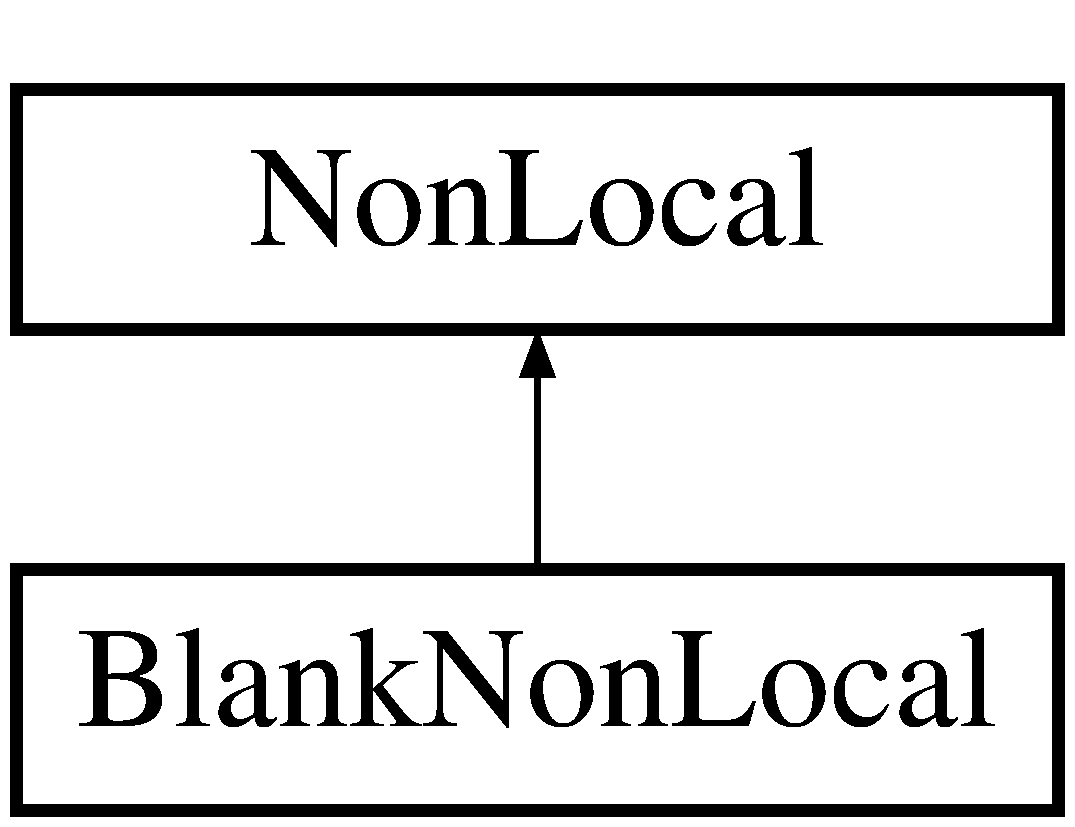
\includegraphics[height=2cm]{class_blank_non_local}
\end{center}
\end{figure}
\subsection*{Public Member Functions}
\begin{DoxyCompactItemize}
\item 
\hypertarget{class_blank_non_local_ab48fb9f176d5b929aaa724e3f5b32a6a}{
void {\bfseries compute} (const \hyperlink{class_scarab_1_1_h_g_1_1_hyperedge}{Hyperedge} \&edge, const vector$<$ vector$<$ int $>$ $>$ \&subder, double \&score, vector$<$ int $>$ \&full\_\-derivation, Sig \&sig) const }
\label{class_blank_non_local_ab48fb9f176d5b929aaa724e3f5b32a6a}

\item 
\hypertarget{class_blank_non_local_a61e2ac11c599d217cacfa5c54bd191b8}{
virtual \hyperlink{struct_hyp}{Hyp} {\bfseries initialize} (const \hyperlink{class_scarab_1_1_h_g_1_1_hypernode}{Hypernode} \&node) const }
\label{class_blank_non_local_a61e2ac11c599d217cacfa5c54bd191b8}

\end{DoxyCompactItemize}


The documentation for this class was generated from the following file:\begin{DoxyCompactItemize}
\item 
hypergraph/CubePruning.h\end{DoxyCompactItemize}

\hypertarget{class_cache}{
\section{Cache$<$ C, V $>$ Class Template Reference}
\label{class_cache}\index{Cache@{Cache}}
}
\subsection*{Public Member Functions}
\begin{DoxyCompactItemize}
\item 
\hypertarget{class_cache_ace98594381db6cd76b3228a73b18190a}{
{\bfseries Cache} (int size)}
\label{class_cache_ace98594381db6cd76b3228a73b18190a}

\item 
\hypertarget{class_cache_ad0a38f45b45b59a772d1e1fd92e59973}{
int {\bfseries size} ()}
\label{class_cache_ad0a38f45b45b59a772d1e1fd92e59973}

\item 
\hypertarget{class_cache_a8d126a64723abe79878befff1c622145}{
const V \& {\bfseries get} (const C \&edge) const }
\label{class_cache_a8d126a64723abe79878befff1c622145}

\item 
\hypertarget{class_cache_a2616bfc563def72da44f91977552ca62}{
V \& {\bfseries get\_\-no\_\-check} (const C \&edge)}
\label{class_cache_a2616bfc563def72da44f91977552ca62}

\item 
\hypertarget{class_cache_a9256aebb417928fbea6090f820d0652d}{
V \& {\bfseries get} (const C \&edge)}
\label{class_cache_a9256aebb417928fbea6090f820d0652d}

\item 
\hypertarget{class_cache_a509df0fde9598a4df9879b5ddb9d93d9}{
V {\bfseries get\_\-value} (const C \&edge) const }
\label{class_cache_a509df0fde9598a4df9879b5ddb9d93d9}

\item 
\hypertarget{class_cache_aeb9ab922add6cf79e2bef1b714f57e8a}{
void {\bfseries set\_\-value} (const C \&edge, V val)}
\label{class_cache_aeb9ab922add6cf79e2bef1b714f57e8a}

\item 
\hypertarget{class_cache_a0864be6a32d0840a4c3009f9ae417902}{
bool {\bfseries has\_\-key} (const C \&edge) const }
\label{class_cache_a0864be6a32d0840a4c3009f9ae417902}

\item 
\hypertarget{class_cache_a213273226c6bb403d33e10e2bc769fe1}{
bool {\bfseries has\_\-key} (int k) const }
\label{class_cache_a213273226c6bb403d33e10e2bc769fe1}

\end{DoxyCompactItemize}
\subsection*{Public Attributes}
\begin{DoxyCompactItemize}
\item 
\hypertarget{class_cache_a4de9009630d4bdc7e78b9db7ea734411}{
vector$<$ V $>$ {\bfseries store}}
\label{class_cache_a4de9009630d4bdc7e78b9db7ea734411}

\item 
\hypertarget{class_cache_a30fcdd51d6ff0cd602cc23d4a12b5348}{
vector$<$ bool $>$ {\bfseries has\_\-value}}
\label{class_cache_a30fcdd51d6ff0cd602cc23d4a12b5348}

\end{DoxyCompactItemize}
\subsubsection*{template$<$class C, class V$>$ class Cache$<$ C, V $>$}



The documentation for this class was generated from the following file:\begin{DoxyCompactItemize}
\item 
hypergraph/EdgeCache.h\end{DoxyCompactItemize}

\hypertarget{struct_candidate}{
\section{Candidate Struct Reference}
\label{struct_candidate}\index{Candidate@{Candidate}}
}
\subsection*{Public Member Functions}
\begin{DoxyCompactItemize}
\item 
\hypertarget{struct_candidate_ac13c7ec637d37b63fc4d6bf3361fd449}{
{\bfseries Candidate} (\hyperlink{struct_hyp}{Hyp} h, const \hyperlink{class_scarab_1_1_h_g_1_1_hyperedge}{Hyperedge} \&e, const vector$<$ int $>$ \&v)}
\label{struct_candidate_ac13c7ec637d37b63fc4d6bf3361fd449}

\item 
\hypertarget{struct_candidate_a5644a3a3d2d92498923ecc443bb4583c}{
bool {\bfseries operator$<$} (const \hyperlink{struct_candidate}{Candidate} \&other) const }
\label{struct_candidate_a5644a3a3d2d92498923ecc443bb4583c}

\end{DoxyCompactItemize}
\subsection*{Public Attributes}
\begin{DoxyCompactItemize}
\item 
\hypertarget{struct_candidate_a22db5a9c75fdebb31827505d6bc7d274}{
\hyperlink{struct_hyp}{Hyp} {\bfseries hyp}}
\label{struct_candidate_a22db5a9c75fdebb31827505d6bc7d274}

\item 
\hypertarget{struct_candidate_acdb6d12cbf33f6e78b97fed5013a181b}{
const \hyperlink{class_scarab_1_1_h_g_1_1_hyperedge}{Hyperedge} \& {\bfseries edge}}
\label{struct_candidate_acdb6d12cbf33f6e78b97fed5013a181b}

\item 
\hypertarget{struct_candidate_afe2daf1c20513a5489d8407492ca7597}{
vector$<$ int $>$ {\bfseries vec}}
\label{struct_candidate_afe2daf1c20513a5489d8407492ca7597}

\end{DoxyCompactItemize}


The documentation for this struct was generated from the following file:\begin{DoxyCompactItemize}
\item 
hypergraph/CubePruning.h\end{DoxyCompactItemize}

\hypertarget{structcandidate__compare}{
\section{candidate\_\-compare Struct Reference}
\label{structcandidate__compare}\index{candidate\_\-compare@{candidate\_\-compare}}
}
\subsection*{Public Member Functions}
\begin{DoxyCompactItemize}
\item 
\hypertarget{structcandidate__compare_ad142d42876f8dd88301ee5f1b3aed03b}{
bool {\bfseries operator()} (const \hyperlink{struct_candidate}{Candidate} $\ast$a, const \hyperlink{struct_candidate}{Candidate} $\ast$b) const }
\label{structcandidate__compare_ad142d42876f8dd88301ee5f1b3aed03b}

\end{DoxyCompactItemize}


The documentation for this struct was generated from the following file:\begin{DoxyCompactItemize}
\item 
hypergraph/CubePruning.h\end{DoxyCompactItemize}

\hypertarget{class_clock}{
\section{Clock Class Reference}
\label{class_clock}\index{Clock@{Clock}}
}
\subsection*{Static Public Member Functions}
\begin{DoxyCompactItemize}
\item 
\hypertarget{class_clock_af45b8db844300755b8c4244a65f60833}{
static double {\bfseries diffclock} (clock\_\-t clock1, clock\_\-t clock2)}
\label{class_clock_af45b8db844300755b8c4244a65f60833}

\end{DoxyCompactItemize}


The documentation for this class was generated from the following file:\begin{DoxyCompactItemize}
\item 
common.h\end{DoxyCompactItemize}

\hypertarget{class_constrainer_dual}{
\section{ConstrainerDual Class Reference}
\label{class_constrainer_dual}\index{ConstrainerDual@{ConstrainerDual}}
}
Inheritance diagram for ConstrainerDual:\begin{figure}[H]
\begin{center}
\leavevmode
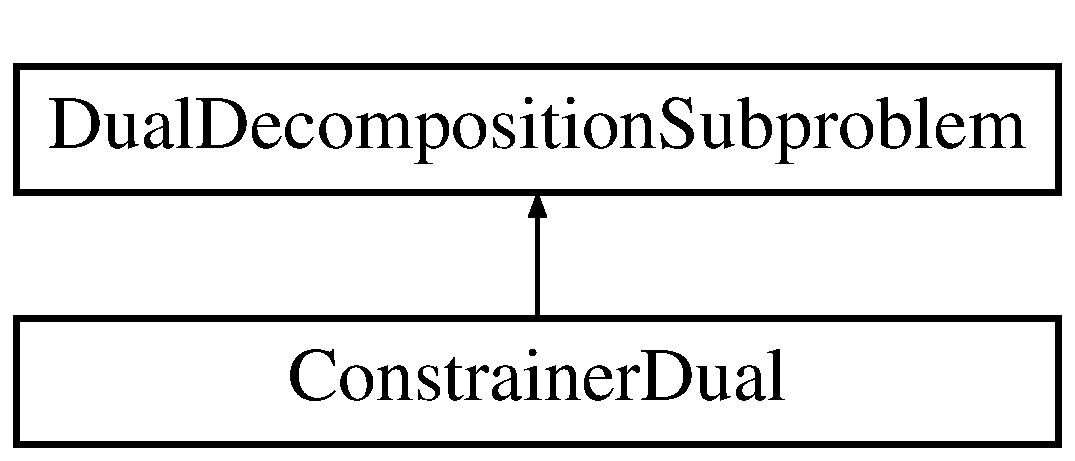
\includegraphics[height=2cm]{class_constrainer_dual}
\end{center}
\end{figure}
\subsection*{Public Member Functions}
\begin{DoxyCompactItemize}
\item 
\hypertarget{class_constrainer_dual_ae74adbb392415eec3451dd5a20820b6b}{
{\bfseries ConstrainerDual} (const \hyperlink{class_tag_constraints}{TagConstraints} \&cons)}
\label{class_constrainer_dual_ae74adbb392415eec3451dd5a20820b6b}

\item 
\hypertarget{class_constrainer_dual_a8cd72c1288fc93a0fec014095ac7252b}{
void {\bfseries solve} (double \&primal, double \&dual, wvector \&, int)}
\label{class_constrainer_dual_a8cd72c1288fc93a0fec014095ac7252b}

\item 
\hypertarget{class_constrainer_dual_a622b99f704a3324133f08521eb4924f5}{
void {\bfseries update\_\-weights} (const wvector \&updates, wvector $\ast$weights, double mult)}
\label{class_constrainer_dual_a622b99f704a3324133f08521eb4924f5}

\end{DoxyCompactItemize}
\subsection*{Protected Attributes}
\begin{DoxyCompactItemize}
\item 
\hypertarget{class_constrainer_dual_abda18ff85d425d3748f49709534ec9ea}{
const \hyperlink{class_tag_constraints}{TagConstraints} \& {\bfseries \_\-tag\_\-constraints}}
\label{class_constrainer_dual_abda18ff85d425d3748f49709534ec9ea}

\item 
\hypertarget{class_constrainer_dual_a4dd6e580712c0b35da77e42e137c7274}{
wvector $\ast$ {\bfseries \_\-cur\_\-weights}}
\label{class_constrainer_dual_a4dd6e580712c0b35da77e42e137c7274}

\end{DoxyCompactItemize}


The documentation for this class was generated from the following files:\begin{DoxyCompactItemize}
\item 
tagger/TagSolvers.h\item 
tagger/TagSolvers.cpp\end{DoxyCompactItemize}

\hypertarget{class_constraint_group}{
\section{ConstraintGroup Class Reference}
\label{class_constraint_group}\index{ConstraintGroup@{ConstraintGroup}}
}
\subsection*{Public Member Functions}
\begin{DoxyCompactItemize}
\item 
\hypertarget{class_constraint_group_a4f37823a56e405c16148c0ba6ae7f114}{
wvector {\bfseries solve\_\-hard} (wvector \&weights) const }
\label{class_constraint_group_a4f37823a56e405c16148c0ba6ae7f114}

\end{DoxyCompactItemize}
\subsection*{Public Attributes}
\begin{DoxyCompactItemize}
\item 
\hypertarget{class_constraint_group_ac96c45d3b2c4c1a6e1068837bc024d9c}{
vector$<$ \hyperlink{struct_possible_tag}{PossibleTag} $>$ {\bfseries group}}
\label{class_constraint_group_ac96c45d3b2c4c1a6e1068837bc024d9c}

\end{DoxyCompactItemize}


The documentation for this class was generated from the following files:\begin{DoxyCompactItemize}
\item 
tagger/TagConstraints.h\item 
tagger/TagConstraints.cpp\end{DoxyCompactItemize}

\hypertarget{class_scarab_1_1_h_g_1_1_controller}{
\section{Scarab::HG::Controller Class Reference}
\label{class_scarab_1_1_h_g_1_1_controller}\index{Scarab::HG::Controller@{Scarab::HG::Controller}}
}
Inheritance diagram for Scarab::HG::Controller:\begin{figure}[H]
\begin{center}
\leavevmode
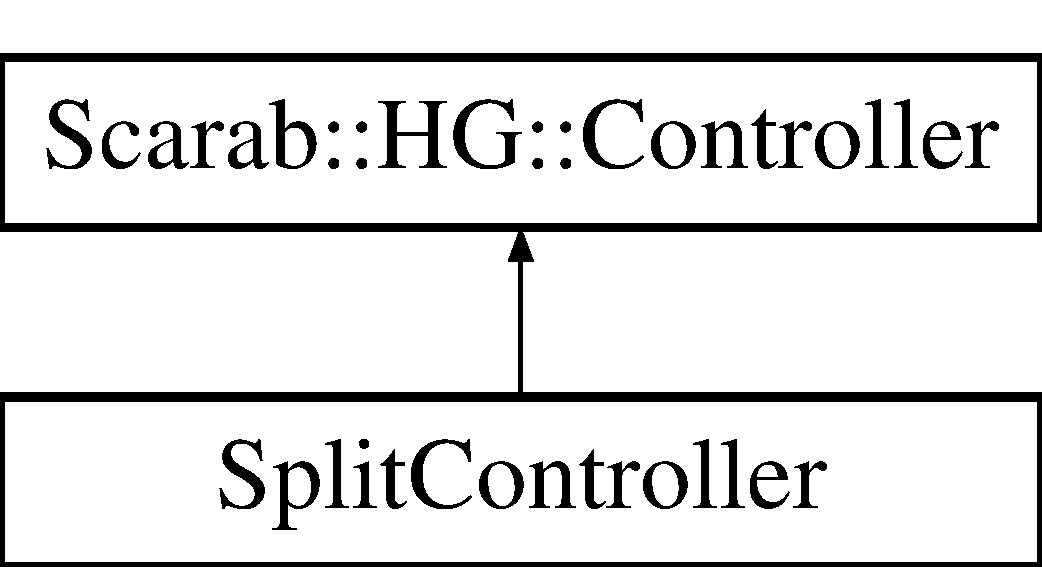
\includegraphics[height=2cm]{class_scarab_1_1_h_g_1_1_controller}
\end{center}
\end{figure}
\subsection*{Public Member Functions}
\begin{DoxyCompactItemize}
\item 
double \hyperlink{class_scarab_1_1_h_g_1_1_controller_a34cfe4b8e7496ffca1cedf64cb3f0a73}{combine} (const \hyperlink{struct_scarab_1_1_h_g_1_1_hypothesis}{Hypothesis} \&a, const \hyperlink{struct_scarab_1_1_h_g_1_1_hypothesis}{Hypothesis} \&b, \hyperlink{struct_scarab_1_1_h_g_1_1_hypothesis}{Hypothesis} \&ret) const 
\item 
\hypertarget{class_scarab_1_1_h_g_1_1_controller_a4b596f04765ad11b691e29383f5fbc3b}{
double {\bfseries combine\_\-back} (const \hyperlink{struct_scarab_1_1_h_g_1_1_hypothesis}{Hypothesis} \&a, const \hyperlink{struct_scarab_1_1_h_g_1_1_hypothesis}{Hypothesis} \&b, \hyperlink{struct_scarab_1_1_h_g_1_1_hypothesis}{Hypothesis} \&ret) const }
\label{class_scarab_1_1_h_g_1_1_controller_a4b596f04765ad11b691e29383f5fbc3b}

\item 
\hypertarget{class_scarab_1_1_h_g_1_1_controller_a5019e9591e6d4e5e29eb4ca6ac42d056}{
virtual void {\bfseries initialize\_\-hypotheses} (const \hyperlink{class_scarab_1_1_h_g_1_1_hypernode}{Hypernode} \&node, vector$<$ \hyperlink{struct_scarab_1_1_h_g_1_1_hypothesis}{Hypothesis} $\ast$ $>$ \&initialize, vector$<$ double $>$ \&scores) const =0}
\label{class_scarab_1_1_h_g_1_1_controller_a5019e9591e6d4e5e29eb4ca6ac42d056}

\item 
\hypertarget{class_scarab_1_1_h_g_1_1_controller_a34e4f087d77d06ee27fff2d3a8435473}{
virtual void {\bfseries initialize\_\-out\_\-root} (vector$<$ \hyperlink{struct_scarab_1_1_h_g_1_1_hypothesis}{Hypothesis} $\ast$ $>$ \&hyps, vector$<$ double $>$ \&scores) const =0}
\label{class_scarab_1_1_h_g_1_1_controller_a34e4f087d77d06ee27fff2d3a8435473}

\item 
\hypertarget{class_scarab_1_1_h_g_1_1_controller_ac4a38bf968379d3dc3f2b95cffabf540}{
virtual double {\bfseries find\_\-best} (vector$<$ \hyperlink{struct_scarab_1_1_h_g_1_1_hypothesis}{Hypothesis} $\ast$ $>$ \&at\_\-root, vector$<$ double $>$ \&scores, \hyperlink{struct_scarab_1_1_h_g_1_1_hypothesis}{Hypothesis} \&best\_\-hyp) const =0}
\label{class_scarab_1_1_h_g_1_1_controller_ac4a38bf968379d3dc3f2b95cffabf540}

\item 
\hypertarget{class_scarab_1_1_h_g_1_1_controller_a3498a09d093e6c6ed993e309db51480a}{
virtual int {\bfseries size} () const =0}
\label{class_scarab_1_1_h_g_1_1_controller_a3498a09d093e6c6ed993e309db51480a}

\item 
\hypertarget{class_scarab_1_1_h_g_1_1_controller_ab4282178c6b8d3670134ab0519eda518}{
virtual int {\bfseries dim} () const =0}
\label{class_scarab_1_1_h_g_1_1_controller_ab4282178c6b8d3670134ab0519eda518}

\end{DoxyCompactItemize}


\subsection{Member Function Documentation}
\hypertarget{class_scarab_1_1_h_g_1_1_controller_a34cfe4b8e7496ffca1cedf64cb3f0a73}{
\index{Scarab::HG::Controller@{Scarab::HG::Controller}!combine@{combine}}
\index{combine@{combine}!Scarab::HG::Controller@{Scarab::HG::Controller}}
\subsubsection[{combine}]{\setlength{\rightskip}{0pt plus 5cm}double Scarab::HG::Controller::combine (const {\bf Hypothesis} \& {\em a}, \/  const {\bf Hypothesis} \& {\em b}, \/  {\bf Hypothesis} \& {\em ret}) const\hspace{0.3cm}{\ttfamily  \mbox{[}inline\mbox{]}}}}
\label{class_scarab_1_1_h_g_1_1_controller_a34cfe4b8e7496ffca1cedf64cb3f0a73}

\begin{DoxyParams}{Parameters}
\item[{\em a}]Left hypothesis \item[{\em b}]Right \hyperlink{struct_scarab_1_1_h_g_1_1_hypothesis}{Hypothesis} \item[{\em ret}]New constructed hypothesis\end{DoxyParams}
\begin{DoxyReturn}{Returns}
Added weight 
\end{DoxyReturn}


The documentation for this class was generated from the following file:\begin{DoxyCompactItemize}
\item 
hypergraph/Hypothesis.h\end{DoxyCompactItemize}

\hypertarget{class_cube_pruning}{
\section{CubePruning Class Reference}
\label{class_cube_pruning}\index{CubePruning@{CubePruning}}
}
\subsection*{Public Member Functions}
\begin{DoxyCompactItemize}
\item 
\hypertarget{class_cube_pruning_af17d9dda17f79a2c44b47501b9d99870}{
{\bfseries CubePruning} (const \hyperlink{class_scarab_1_1_h_g_1_1_h_graph}{HGraph} \&forest, const \hyperlink{class_cache}{Cache}$<$ \hyperlink{class_scarab_1_1_h_g_1_1_hyperedge}{Hyperedge}, double $>$ \&weights, const \hyperlink{class_non_local}{NonLocal} \&non\_\-local, int k, int ratio)}
\label{class_cube_pruning_af17d9dda17f79a2c44b47501b9d99870}

\item 
\hypertarget{class_cube_pruning_a0e8d07fc09d695095be5b70780db95d6}{
void {\bfseries get\_\-derivation} (vector$<$ int $>$ \&der)}
\label{class_cube_pruning_a0e8d07fc09d695095be5b70780db95d6}

\item 
\hypertarget{class_cube_pruning_adf80c0c689d075765f250649433833e4}{
double {\bfseries parse} ()}
\label{class_cube_pruning_adf80c0c689d075765f250649433833e4}

\item 
\hypertarget{class_cube_pruning_ab949710c0d8e552cbadbe837b1b62d47}{
void {\bfseries run} (const \hyperlink{class_scarab_1_1_h_g_1_1_hypernode}{Hypernode} \&cur\_\-node, vector$<$ \hyperlink{struct_hyp}{Hyp} $>$ \&kbest\_\-hyps)}
\label{class_cube_pruning_ab949710c0d8e552cbadbe837b1b62d47}

\item 
\hypertarget{class_cube_pruning_a14a4e797c638d07744dc328cf2ce568e}{
void {\bfseries init\_\-cube} (const \hyperlink{class_scarab_1_1_h_g_1_1_hypernode}{Hypernode} \&cur\_\-node, Candidates \&cands)}
\label{class_cube_pruning_a14a4e797c638d07744dc328cf2ce568e}

\item 
\hypertarget{class_cube_pruning_abe8c53bd14fe4ad98ff6388f38a849cb}{
void {\bfseries kbest} (Candidates \&cands, vector$<$ \hyperlink{struct_hyp}{Hyp} $>$ \&)}
\label{class_cube_pruning_abe8c53bd14fe4ad98ff6388f38a849cb}

\item 
\hypertarget{class_cube_pruning_a5d3ab59862953b9000154e9c07c69634}{
void {\bfseries next} (const \hyperlink{class_scarab_1_1_h_g_1_1_hyperedge}{Hyperedge} \&cedge, const vector$<$ int $>$ \&cvecj, Candidates \&cands)}
\label{class_cube_pruning_a5d3ab59862953b9000154e9c07c69634}

\item 
\hypertarget{class_cube_pruning_aa7d26357be4241b594f9eb24ac52da22}{
bool {\bfseries gethyp} (const \hyperlink{class_scarab_1_1_h_g_1_1_hyperedge}{Hyperedge} \&cedge, const vector$<$ int $>$ \&vecj, \hyperlink{struct_hyp}{Hyp} \&item)}
\label{class_cube_pruning_aa7d26357be4241b594f9eb24ac52da22}

\end{DoxyCompactItemize}


The documentation for this class was generated from the following files:\begin{DoxyCompactItemize}
\item 
hypergraph/CubePruning.h\item 
hypergraph/CubePruning.cpp\end{DoxyCompactItemize}

\hypertarget{class_decode}{
\section{Decode Class Reference}
\label{class_decode}\index{Decode@{Decode}}
}
Inheritance diagram for Decode:\begin{figure}[H]
\begin{center}
\leavevmode
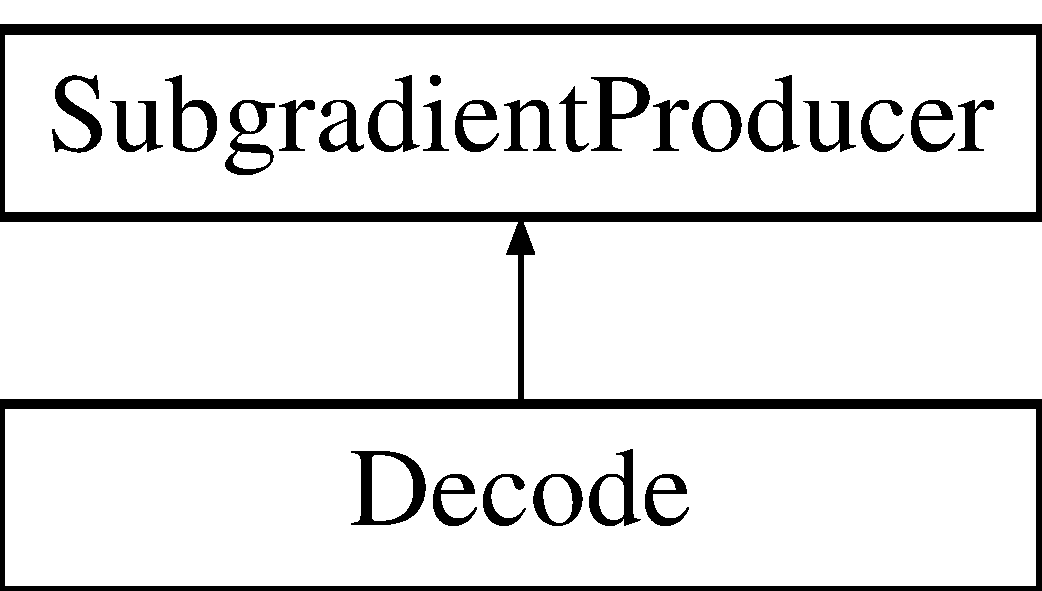
\includegraphics[height=2cm]{class_decode}
\end{center}
\end{figure}
\subsection*{Public Member Functions}
\begin{DoxyCompactItemize}
\item 
\hypertarget{class_decode_a57bd53ddaf49e2fe4b86a7aad782110f}{
{\bfseries Decode} (const \hyperlink{class_forest}{Forest} \&forest, const \hyperlink{class_forest_lattice}{ForestLattice} \&lattice, const wvector \&weight, \hyperlink{class_ngram_cache}{NgramCache} \&lm)}
\label{class_decode_a57bd53ddaf49e2fe4b86a7aad782110f}

\item 
\hypertarget{class_decode_a6d86f91ee2c591c54ce2bb97c1dd6888}{
void {\bfseries solve} (double \&primal, double \&dual, wvector \&, int, bool, bool \&)}
\label{class_decode_a6d86f91ee2c591c54ce2bb97c1dd6888}

\item 
\hypertarget{class_decode_a9beca60221318f111b7f4d5acca8e329}{
void {\bfseries update\_\-weights} (const wvector \&updates, wvector $\ast$weights)}
\label{class_decode_a9beca60221318f111b7f4d5acca8e329}

\end{DoxyCompactItemize}


The documentation for this class was generated from the following files:\begin{DoxyCompactItemize}
\item 
trans\_\-decode/Decode.h\item 
trans\_\-decode/Decode.cpp\end{DoxyCompactItemize}

\hypertarget{struct_dependency}{
\section{Dependency Struct Reference}
\label{struct_dependency}\index{Dependency@{Dependency}}
}
\subsection*{Public Member Functions}
\begin{DoxyCompactItemize}
\item 
\hypertarget{struct_dependency_a92ebdf715c4c81e556bc274f86027400}{
{\bfseries Dependency} (int l, int h, int m)}
\label{struct_dependency_a92ebdf715c4c81e556bc274f86027400}

\item 
\hypertarget{struct_dependency_a38ba361a116c72f4e41298b6320a6540}{
int {\bfseries id} () const }
\label{struct_dependency_a38ba361a116c72f4e41298b6320a6540}

\end{DoxyCompactItemize}
\subsection*{Public Attributes}
\begin{DoxyCompactItemize}
\item 
\hypertarget{struct_dependency_ae50c91ea1c7f2a16a29e7ecf9cf0a6ba}{
int {\bfseries head}}
\label{struct_dependency_ae50c91ea1c7f2a16a29e7ecf9cf0a6ba}

\item 
\hypertarget{struct_dependency_a45e806cfc00a3bcce4d5ebaab52c1f77}{
int {\bfseries mod}}
\label{struct_dependency_a45e806cfc00a3bcce4d5ebaab52c1f77}

\item 
\hypertarget{struct_dependency_a95f049533781d9ae8fea8f447e4739fe}{
int {\bfseries length}}
\label{struct_dependency_a95f049533781d9ae8fea8f447e4739fe}

\end{DoxyCompactItemize}


The documentation for this struct was generated from the following file:\begin{DoxyCompactItemize}
\item 
parse/DepParser.h\end{DoxyCompactItemize}

\hypertarget{class_dep_parser}{
\section{DepParser Class Reference}
\label{class_dep_parser}\index{DepParser@{DepParser}}
}
Inheritance diagram for DepParser:\begin{figure}[H]
\begin{center}
\leavevmode
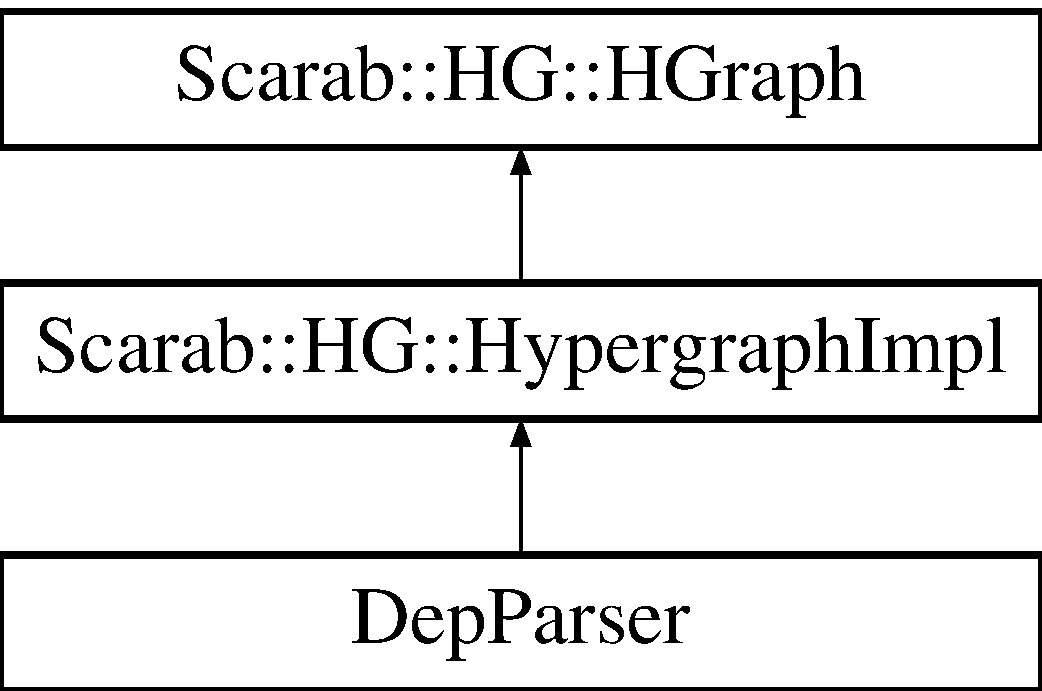
\includegraphics[height=3cm]{class_dep_parser}
\end{center}
\end{figure}
\subsection*{Public Member Functions}
\begin{DoxyCompactItemize}
\item 
void \hyperlink{class_dep_parser_a9aebbbde821bad423b6c01cc12f02a2c}{print} () const 
\item 
\hypertarget{class_dep_parser_a6131e95a8ec7b07f7a4d68dae224d52f}{
void {\bfseries set\_\-up} (const Hypergraph \&hgraph)}
\label{class_dep_parser_a6131e95a8ec7b07f7a4d68dae224d52f}

\item 
\hypertarget{class_dep_parser_aaec31758432c2d3336d2164996571688}{
const Hypergraph \& {\bfseries hypergraph} () const }
\label{class_dep_parser_aaec31758432c2d3336d2164996571688}

\item 
\hypertarget{class_dep_parser_aa64f67830bf4c3bf9936ba6056dfdff0}{
vector$<$ \hyperlink{struct_dependency}{Dependency} $>$ {\bfseries dependencies} () const }
\label{class_dep_parser_aa64f67830bf4c3bf9936ba6056dfdff0}

\item 
\hypertarget{class_dep_parser_aaff55cf38fd9b1fbfb22090ddeb72ba8}{
uint {\bfseries num\_\-deps} () const }
\label{class_dep_parser_aaff55cf38fd9b1fbfb22090ddeb72ba8}

\item 
\hypertarget{class_dep_parser_a86b99d09d76b7d6f8733b208e9f32822}{
uint {\bfseries sent\_\-length} () const }
\label{class_dep_parser_a86b99d09d76b7d6f8733b208e9f32822}

\item 
\hypertarget{class_dep_parser_a49afcb1a83a3c924869faf34cd9e968e}{
\hyperlink{struct_dependency}{Dependency} {\bfseries make\_\-dep} (int head, int mod) const }
\label{class_dep_parser_a49afcb1a83a3c924869faf34cd9e968e}

\item 
\hypertarget{class_dep_parser_a9fa2f0bf24cd870404f0a99b5926c558}{
const vector$<$ const \hyperlink{class_scarab_1_1_h_g_1_1_hyperedge}{Hyperedge} $\ast$ $>$ \& {\bfseries dep\_\-to\_\-edge} (const \hyperlink{struct_dependency}{Dependency} \&dep) const }
\label{class_dep_parser_a9fa2f0bf24cd870404f0a99b5926c558}

\item 
\hypertarget{class_dep_parser_aa5ff87f99326c60633fb8e26d1737776}{
const \hyperlink{struct_dependency}{Dependency} \& {\bfseries edge\_\-to\_\-dep} (const \hyperlink{class_scarab_1_1_h_g_1_1_hyperedge}{Hyperedge} \&edge) const }
\label{class_dep_parser_aa5ff87f99326c60633fb8e26d1737776}

\item 
\hypertarget{class_dep_parser_abd0b9171e59c1c40cdb58807a46a5449}{
bool {\bfseries edge\_\-has\_\-dep} (const \hyperlink{class_scarab_1_1_h_g_1_1_hyperedge}{Hyperedge} \&edge) const }
\label{class_dep_parser_abd0b9171e59c1c40cdb58807a46a5449}

\end{DoxyCompactItemize}
\subsection*{Protected Member Functions}
\begin{DoxyCompactItemize}
\item 
\hypertarget{class_dep_parser_a04d313d931d1e8b0bac3a36ca7be469b}{
void {\bfseries make\_\-edge} (const Hypergraph\_\-Edge \&edge, const \hyperlink{class_scarab_1_1_h_g_1_1_hyperedge}{Scarab::HG::Hyperedge} $\ast$our\_\-edge)}
\label{class_dep_parser_a04d313d931d1e8b0bac3a36ca7be469b}

\end{DoxyCompactItemize}


\subsection{Member Function Documentation}
\hypertarget{class_dep_parser_a9aebbbde821bad423b6c01cc12f02a2c}{
\index{DepParser@{DepParser}!print@{print}}
\index{print@{print}!DepParser@{DepParser}}
\subsubsection[{print}]{\setlength{\rightskip}{0pt plus 5cm}void DepParser::print () const\hspace{0.3cm}{\ttfamily  \mbox{[}inline, virtual\mbox{]}}}}
\label{class_dep_parser_a9aebbbde821bad423b6c01cc12f02a2c}
Display the hypergraph for debugging. 

Implements \hyperlink{class_scarab_1_1_h_g_1_1_h_graph_ab5aa11c932b28864b56f28e0babbc1c1}{Scarab::HG::HGraph}.



The documentation for this class was generated from the following file:\begin{DoxyCompactItemize}
\item 
parse/DepParser.h\end{DoxyCompactItemize}

\hypertarget{struct_scarab_1_1_h_g_1_1_dep_parser_l_p}{
\section{Scarab::HG::DepParserLP Struct Reference}
\label{struct_scarab_1_1_h_g_1_1_dep_parser_l_p}\index{Scarab::HG::DepParserLP@{Scarab::HG::DepParserLP}}
}
\subsection*{Public Member Functions}
\begin{DoxyCompactItemize}
\item 
\hypertarget{struct_scarab_1_1_h_g_1_1_dep_parser_l_p_aaec1248e50de35594c4a20e89a782e95}{
{\bfseries DepParserLP} (const \hyperlink{class_dep_parser}{DepParser} \&parser, const \hyperlink{struct_scarab_1_1_h_g_1_1_hypergraph_l_p}{HypergraphLP} \&hyper\_\-lp)}
\label{struct_scarab_1_1_h_g_1_1_dep_parser_l_p_aaec1248e50de35594c4a20e89a782e95}

\end{DoxyCompactItemize}
\subsection*{Public Attributes}
\begin{DoxyCompactItemize}
\item 
\hypertarget{struct_scarab_1_1_h_g_1_1_dep_parser_l_p_af31e9d91e3407559cd2588bfef2296e3}{
\hyperlink{class_cache}{Cache}$<$ \hyperlink{struct_dependency}{Dependency}, GRBVar $>$ {\bfseries dep\_\-vars}}
\label{struct_scarab_1_1_h_g_1_1_dep_parser_l_p_af31e9d91e3407559cd2588bfef2296e3}

\item 
\hypertarget{struct_scarab_1_1_h_g_1_1_dep_parser_l_p_a93d0f269dabdd6fe83c68ee51baafb62}{
const \hyperlink{class_dep_parser}{DepParser} \& {\bfseries p}}
\label{struct_scarab_1_1_h_g_1_1_dep_parser_l_p_a93d0f269dabdd6fe83c68ee51baafb62}

\item 
\hypertarget{struct_scarab_1_1_h_g_1_1_dep_parser_l_p_acab7463a0d1349c5a1250ac0653c0569}{
const \hyperlink{struct_scarab_1_1_h_g_1_1_hypergraph_l_p}{HypergraphLP} \& {\bfseries h\_\-lp}}
\label{struct_scarab_1_1_h_g_1_1_dep_parser_l_p_acab7463a0d1349c5a1250ac0653c0569}

\end{DoxyCompactItemize}


The documentation for this struct was generated from the following file:\begin{DoxyCompactItemize}
\item 
lp/DepParseLP.h\end{DoxyCompactItemize}

\hypertarget{class_scarab_1_1_h_g_1_1_dep_parser_l_p_builder}{
\section{Scarab::HG::DepParserLPBuilder Class Reference}
\label{class_scarab_1_1_h_g_1_1_dep_parser_l_p_builder}\index{Scarab::HG::DepParserLPBuilder@{Scarab::HG::DepParserLPBuilder}}
}
\subsection*{Static Public Member Functions}
\begin{DoxyCompactItemize}
\item 
\hypertarget{class_scarab_1_1_h_g_1_1_dep_parser_l_p_builder_a8864b215a93fa51c4df30669dacb0ddc}{
static void {\bfseries show\_\-results} (const \hyperlink{struct_scarab_1_1_h_g_1_1_dep_parser_l_p}{DepParserLP} \&lp\_\-vars)}
\label{class_scarab_1_1_h_g_1_1_dep_parser_l_p_builder_a8864b215a93fa51c4df30669dacb0ddc}

\item 
\hypertarget{class_scarab_1_1_h_g_1_1_dep_parser_l_p_builder_a862127f9347f244103941a119747b810}{
static \hyperlink{struct_scarab_1_1_h_g_1_1_dep_parser_l_p}{DepParserLP} $\ast$ {\bfseries add\_\-parse} (const \hyperlink{class_dep_parser}{DepParser} \&parser, const \hyperlink{class_cache}{Cache}$<$ \hyperlink{class_scarab_1_1_h_g_1_1_hyperedge}{Hyperedge}, double $>$ \&weights, string prefix, GRBModel \&model, int var\_\-type)}
\label{class_scarab_1_1_h_g_1_1_dep_parser_l_p_builder_a862127f9347f244103941a119747b810}

\end{DoxyCompactItemize}


The documentation for this class was generated from the following files:\begin{DoxyCompactItemize}
\item 
lp/DepParseLP.h\item 
lp/DepParseLP.cpp\end{DoxyCompactItemize}

\hypertarget{class_dual_decomposition}{
\section{DualDecomposition Class Reference}
\label{class_dual_decomposition}\index{DualDecomposition@{DualDecomposition}}
}
\subsection*{Public Member Functions}
\begin{DoxyCompactItemize}
\item 
\hypertarget{class_dual_decomposition_a652c2229bad83ce7b135aa06ef1283a5}{
{\bfseries DualDecomposition} (\hyperlink{class_dual_decomposition_subproblem}{DualDecompositionSubproblem} \&s1, \hyperlink{class_dual_decomposition_subproblem}{DualDecompositionSubproblem} \&s2)}
\label{class_dual_decomposition_a652c2229bad83ce7b135aa06ef1283a5}

\item 
\hypertarget{class_dual_decomposition_a0013544261cba254dc2ca2c68cbb1679}{
void {\bfseries solve} (int example)}
\label{class_dual_decomposition_a0013544261cba254dc2ca2c68cbb1679}

\end{DoxyCompactItemize}


The documentation for this class was generated from the following file:\begin{DoxyCompactItemize}
\item 
optimization/DualDecomposition.h\end{DoxyCompactItemize}

\hypertarget{class_dual_decomposition_runner}{
\section{DualDecompositionRunner Class Reference}
\label{class_dual_decomposition_runner}\index{DualDecompositionRunner@{DualDecompositionRunner}}
}
Inheritance diagram for DualDecompositionRunner:\begin{figure}[H]
\begin{center}
\leavevmode
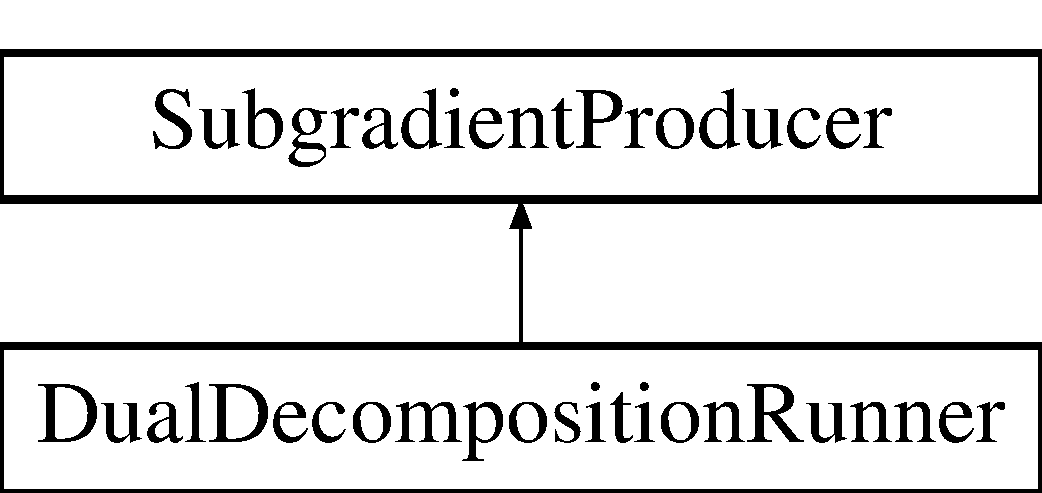
\includegraphics[height=2cm]{class_dual_decomposition_runner}
\end{center}
\end{figure}
\subsection*{Public Member Functions}
\begin{DoxyCompactItemize}
\item 
\hypertarget{class_dual_decomposition_runner_ad0af4c8b1a73612770d329cf560af9d1}{
{\bfseries DualDecompositionRunner} (\hyperlink{class_dual_decomposition_subproblem}{DualDecompositionSubproblem} \&s1, \hyperlink{class_dual_decomposition_subproblem}{DualDecompositionSubproblem} \&s2)}
\label{class_dual_decomposition_runner_ad0af4c8b1a73612770d329cf560af9d1}

\item 
\hypertarget{class_dual_decomposition_runner_a4bcec895359acf32000d42155c4593ef}{
void {\bfseries solve} (double \&primal, double \&dual, wvector \&subgrad, int round, bool is\_\-stuck, bool \&bump\_\-rate)}
\label{class_dual_decomposition_runner_a4bcec895359acf32000d42155c4593ef}

\item 
\hypertarget{class_dual_decomposition_runner_a3cdf7ce33f6454f9fee9fb9c3287c5ac}{
void {\bfseries update\_\-weights} (const wvector \&updates, wvector $\ast$weights)}
\label{class_dual_decomposition_runner_a3cdf7ce33f6454f9fee9fb9c3287c5ac}

\end{DoxyCompactItemize}
\subsection*{Public Attributes}
\begin{DoxyCompactItemize}
\item 
\hypertarget{class_dual_decomposition_runner_a13371fbf1e5109e8a9d920d2ed0b7bea}{
\hyperlink{class_dual_decomposition_subproblem}{DualDecompositionSubproblem} \& {\bfseries \_\-sub\_\-producer1}}
\label{class_dual_decomposition_runner_a13371fbf1e5109e8a9d920d2ed0b7bea}

\item 
\hypertarget{class_dual_decomposition_runner_a988b68df84c131bc47d142ae8638fbd1}{
\hyperlink{class_dual_decomposition_subproblem}{DualDecompositionSubproblem} \& {\bfseries \_\-sub\_\-producer2}}
\label{class_dual_decomposition_runner_a988b68df84c131bc47d142ae8638fbd1}

\end{DoxyCompactItemize}


The documentation for this class was generated from the following file:\begin{DoxyCompactItemize}
\item 
optimization/DualDecomposition.h\end{DoxyCompactItemize}

\hypertarget{class_dual_decomposition_subproblem}{
\section{DualDecompositionSubproblem Class Reference}
\label{class_dual_decomposition_subproblem}\index{DualDecompositionSubproblem@{DualDecompositionSubproblem}}
}
Inheritance diagram for DualDecompositionSubproblem:\begin{figure}[H]
\begin{center}
\leavevmode
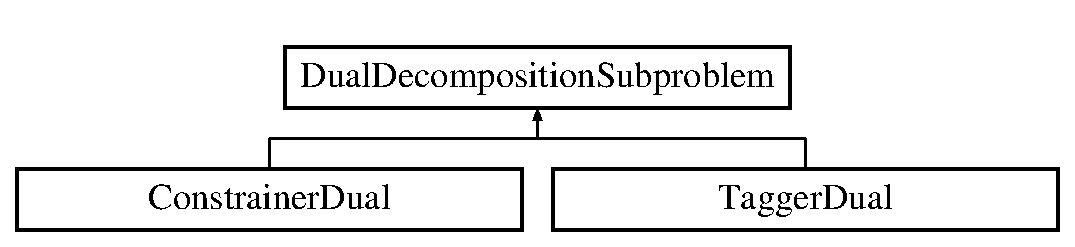
\includegraphics[height=2cm]{class_dual_decomposition_subproblem}
\end{center}
\end{figure}
\subsection*{Public Member Functions}
\begin{DoxyCompactItemize}
\item 
\hypertarget{class_dual_decomposition_subproblem_aac234786c13091898be348dc0056a036}{
virtual void {\bfseries solve} (double \&primal, double \&dual, wvector \&, int)=0}
\label{class_dual_decomposition_subproblem_aac234786c13091898be348dc0056a036}

\item 
\hypertarget{class_dual_decomposition_subproblem_a6d26fcb23023d5b03d54b3d191531b02}{
virtual void {\bfseries update\_\-weights} (const wvector \&updates, wvector $\ast$weights, double mult)=0}
\label{class_dual_decomposition_subproblem_a6d26fcb23023d5b03d54b3d191531b02}

\end{DoxyCompactItemize}


The documentation for this class was generated from the following file:\begin{DoxyCompactItemize}
\item 
optimization/DualDecomposition.h\end{DoxyCompactItemize}

\hypertarget{struct_eisner_node}{
\section{EisnerNode Struct Reference}
\label{struct_eisner_node}\index{EisnerNode@{EisnerNode}}
}
\subsection*{Public Member Functions}
\begin{DoxyCompactItemize}
\item 
\hypertarget{struct_eisner_node_a38fe91d99e35e7d8a6bda3c1bb45f3d6}{
string {\bfseries name} ()}
\label{struct_eisner_node_a38fe91d99e35e7d8a6bda3c1bb45f3d6}

\item 
\hypertarget{struct_eisner_node_a16b4c3b130c5cacf4639fb8fc01d1894}{
{\bfseries EisnerNode} (\hyperlink{struct_span}{Span} ns, Direction d\_\-in, Shape s\_\-in)}
\label{struct_eisner_node_a16b4c3b130c5cacf4639fb8fc01d1894}

\item 
\hypertarget{struct_eisner_node_a8ede91dac02b136ef673afbb68566623}{
bool {\bfseries operator$<$} (const \hyperlink{struct_eisner_node}{EisnerNode} \&other) const }
\label{struct_eisner_node_a8ede91dac02b136ef673afbb68566623}

\end{DoxyCompactItemize}
\subsection*{Public Attributes}
\begin{DoxyCompactItemize}
\item 
\hypertarget{struct_eisner_node_a1e3b0f200089af99ca744d6d0a9c7f72}{
\hyperlink{struct_span}{Span} {\bfseries node\_\-span}}
\label{struct_eisner_node_a1e3b0f200089af99ca744d6d0a9c7f72}

\item 
\hypertarget{struct_eisner_node_a0013abe4607fb7979aa1d915a58868a1}{
Direction {\bfseries d}}
\label{struct_eisner_node_a0013abe4607fb7979aa1d915a58868a1}

\item 
\hypertarget{struct_eisner_node_a682edd0712304525c84939b820a141d3}{
Shape {\bfseries s}}
\label{struct_eisner_node_a682edd0712304525c84939b820a141d3}

\end{DoxyCompactItemize}


The documentation for this struct was generated from the following file:\begin{DoxyCompactItemize}
\item 
parse/EisnerToHypergraph.h\end{DoxyCompactItemize}

\hypertarget{class_eisner_to_hypergraph}{
\section{EisnerToHypergraph Class Reference}
\label{class_eisner_to_hypergraph}\index{EisnerToHypergraph@{EisnerToHypergraph}}
}
\subsection*{Public Member Functions}
\begin{DoxyCompactItemize}
\item 
\hypertarget{class_eisner_to_hypergraph_ac4c11a966298244ad74965dd35596c4c}{
{\bfseries EisnerToHypergraph} (const vector$<$ int $>$ \&sent, vector$<$ vector$<$ vector$<$ double $>$ $>$ $>$ \&weights)}
\label{class_eisner_to_hypergraph_ac4c11a966298244ad74965dd35596c4c}

\item 
\hypertarget{class_eisner_to_hypergraph_a8344d534c1b3d5f2795578c771fe4d31}{
void {\bfseries convert} (Hypergraph \&\_\-forest)}
\label{class_eisner_to_hypergraph_a8344d534c1b3d5f2795578c771fe4d31}

\end{DoxyCompactItemize}
\subsection*{Public Attributes}
\begin{DoxyCompactItemize}
\item 
\hypertarget{class_eisner_to_hypergraph_a47df02a8804876cc0e33b55681b9a2f0}{
Hypergraph {\bfseries hgraph}}
\label{class_eisner_to_hypergraph_a47df02a8804876cc0e33b55681b9a2f0}

\end{DoxyCompactItemize}


The documentation for this class was generated from the following files:\begin{DoxyCompactItemize}
\item 
parse/EisnerToHypergraph.h\item 
parse/EisnerToHypergraph.cpp\end{DoxyCompactItemize}

\hypertarget{class_scarab_1_1_h_g_1_1_extend_c_k_y}{
\section{Scarab::HG::ExtendCKY Class Reference}
\label{class_scarab_1_1_h_g_1_1_extend_c_k_y}\index{Scarab::HG::ExtendCKY@{Scarab::HG::ExtendCKY}}
}
\subsection*{Public Member Functions}
\begin{DoxyCompactItemize}
\item 
\hypertarget{class_scarab_1_1_h_g_1_1_extend_c_k_y_a393c61229e019cb875ba6b7b6b176aff}{
{\bfseries ExtendCKY} (const \hyperlink{class_scarab_1_1_h_g_1_1_h_graph}{HGraph} \&forest, const \hyperlink{class_cache}{Cache}$<$ \hyperlink{class_scarab_1_1_h_g_1_1_hyperedge}{Hyperedge}, double $>$ \&edge\_\-weights, const \hyperlink{class_scarab_1_1_h_g_1_1_controller}{Controller} \&cont)}
\label{class_scarab_1_1_h_g_1_1_extend_c_k_y_a393c61229e019cb875ba6b7b6b176aff}

\item 
\hypertarget{class_scarab_1_1_h_g_1_1_extend_c_k_y_ae72fa6e6e0bb69464c575bd5225b1423}{
double {\bfseries best\_\-path} (\hyperlink{class_cache}{NodeBackCache} \&back\_\-pointers)}
\label{class_scarab_1_1_h_g_1_1_extend_c_k_y_ae72fa6e6e0bb69464c575bd5225b1423}

\item 
\hypertarget{class_scarab_1_1_h_g_1_1_extend_c_k_y_a038f64197127bc278e6a25c4565c72bd}{
void {\bfseries outside} ()}
\label{class_scarab_1_1_h_g_1_1_extend_c_k_y_a038f64197127bc278e6a25c4565c72bd}

\end{DoxyCompactItemize}
\subsection*{Public Attributes}
\begin{DoxyCompactItemize}
\item 
\hypertarget{class_scarab_1_1_h_g_1_1_extend_c_k_y_a008898035d6c06258e25a502fbfd7377}{
\hyperlink{class_cache}{Cache}$<$ \hyperlink{class_scarab_1_1_h_g_1_1_hypernode}{Hypernode}, \hyperlink{class_scarab_1_1_h_g_1_1_best_hyp}{BestHyp} $>$ {\bfseries \_\-outside\_\-memo\_\-table}}
\label{class_scarab_1_1_h_g_1_1_extend_c_k_y_a008898035d6c06258e25a502fbfd7377}

\item 
\hypertarget{class_scarab_1_1_h_g_1_1_extend_c_k_y_a554aa074d56b38acb561fda8584b9b8a}{
\hyperlink{class_cache}{Cache}$<$ \hyperlink{class_scarab_1_1_h_g_1_1_hyperedge}{Hyperedge}, vector$<$ \hyperlink{class_scarab_1_1_h_g_1_1_best_hyp}{BestHyp} $>$ $>$ {\bfseries \_\-outside\_\-edge\_\-memo\_\-table}}
\label{class_scarab_1_1_h_g_1_1_extend_c_k_y_a554aa074d56b38acb561fda8584b9b8a}

\end{DoxyCompactItemize}


The documentation for this class was generated from the following files:\begin{DoxyCompactItemize}
\item 
hypergraph/ExtendCKY.h\item 
hypergraph/ExtendCKY.cpp\end{DoxyCompactItemize}

\hypertarget{class_forest}{
\section{Forest Class Reference}
\label{class_forest}\index{Forest@{Forest}}
}
Inheritance diagram for Forest:\begin{figure}[H]
\begin{center}
\leavevmode
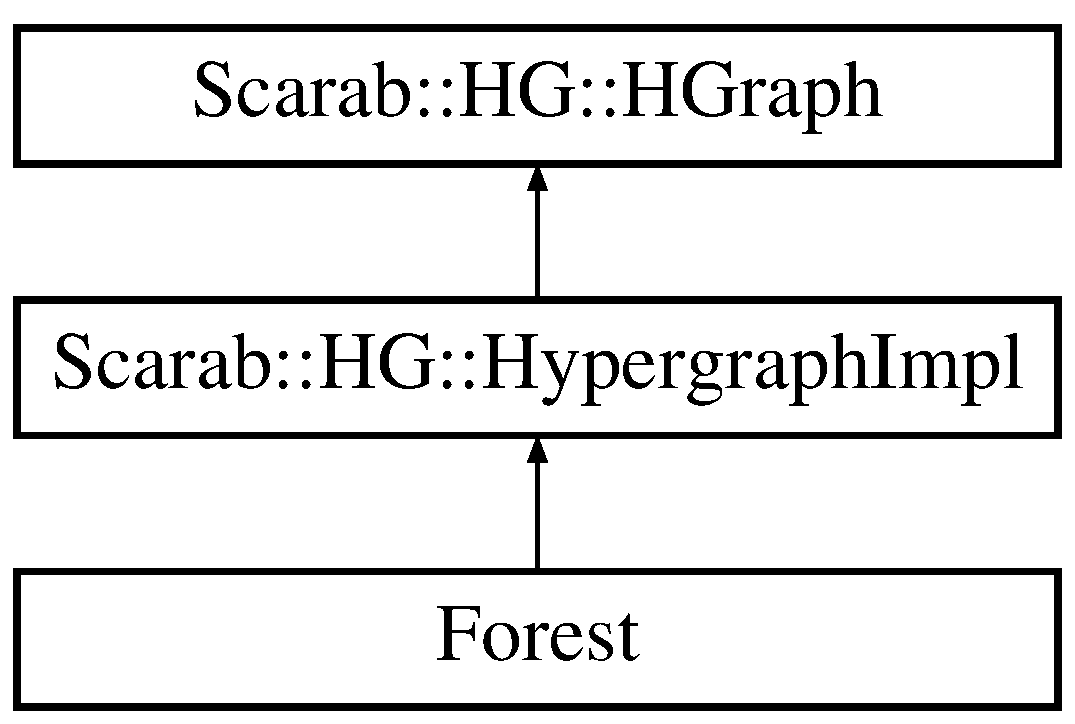
\includegraphics[height=3cm]{class_forest}
\end{center}
\end{figure}
\subsection*{Public Member Functions}
\begin{DoxyCompactItemize}
\item 
void \hyperlink{class_forest_a621a1a65d0f877bb33b15c79f9e24c4d}{print} () const 
\item 
\hypertarget{class_forest_a4cc0cf94c18913eadd0b36f3dcf68cef}{
void {\bfseries append\_\-end\_\-nodes} ()}
\label{class_forest_a4cc0cf94c18913eadd0b36f3dcf68cef}

\end{DoxyCompactItemize}
\subsection*{Static Public Member Functions}
\begin{DoxyCompactItemize}
\item 
\hypertarget{class_forest_a1b9ddc0e03c1ccfcc73987fe9378fa84}{
static \hyperlink{class_forest}{Forest} {\bfseries from\_\-file} (const char $\ast$file\_\-name)}
\label{class_forest_a1b9ddc0e03c1ccfcc73987fe9378fa84}

\end{DoxyCompactItemize}
\subsection*{Protected Member Functions}
\begin{DoxyCompactItemize}
\item 
\hypertarget{class_forest_ab40070ea9e3885d252fb7848c11f27ef}{
\hyperlink{class_scarab_1_1_h_g_1_1_hypernode}{Scarab::HG::Hypernode} $\ast$ {\bfseries make\_\-node} (const Hypergraph\_\-Node \&node, wvector $\ast$features)}
\label{class_forest_ab40070ea9e3885d252fb7848c11f27ef}

\end{DoxyCompactItemize}


\subsection{Member Function Documentation}
\hypertarget{class_forest_a621a1a65d0f877bb33b15c79f9e24c4d}{
\index{Forest@{Forest}!print@{print}}
\index{print@{print}!Forest@{Forest}}
\subsubsection[{print}]{\setlength{\rightskip}{0pt plus 5cm}void Forest::print () const\hspace{0.3cm}{\ttfamily  \mbox{[}virtual\mbox{]}}}}
\label{class_forest_a621a1a65d0f877bb33b15c79f9e24c4d}
Display the hypergraph for debugging. 

Implements \hyperlink{class_scarab_1_1_h_g_1_1_h_graph_ab5aa11c932b28864b56f28e0babbc1c1}{Scarab::HG::HGraph}.



The documentation for this class was generated from the following files:\begin{DoxyCompactItemize}
\item 
transforest/Forest.h\item 
transforest/Forest.cpp\end{DoxyCompactItemize}

\hypertarget{class_forest_lattice}{
\section{ForestLattice Class Reference}
\label{class_forest_lattice}\index{ForestLattice@{ForestLattice}}
}
\subsection*{Public Member Functions}
\begin{DoxyCompactItemize}
\item 
\hypertarget{class_forest_lattice_ad14bc799ac36b716c292f410e1609462}{
string {\bfseries get\_\-word} (int word\_\-num) const }
\label{class_forest_lattice_ad14bc799ac36b716c292f410e1609462}

\item 
\hypertarget{class_forest_lattice_a8303ce943210d4a62132f1e4054b7191}{
const \hyperlink{class_scarab_1_1_graph_1_1_graph}{Graph} \& {\bfseries get\_\-graph} () const }
\label{class_forest_lattice_a8303ce943210d4a62132f1e4054b7191}

\item 
\hypertarget{class_forest_lattice_a744558d8489b4428c44275f0966d587e}{
const \hyperlink{class_scarab_1_1_graph_1_1_graphnode}{Graphnode} \& {\bfseries node} (int i) const }
\label{class_forest_lattice_a744558d8489b4428c44275f0966d587e}

\item 
\hypertarget{class_forest_lattice_a8afba92a7fb437a93db30b2336ad3824}{
bool {\bfseries is\_\-phrase\_\-node} (int n) const }
\label{class_forest_lattice_a8afba92a7fb437a93db30b2336ad3824}

\item 
\hypertarget{class_forest_lattice_a9d82493dff97186334923b582999f63c}{
bool {\bfseries is\_\-word} (int w) const }
\label{class_forest_lattice_a9d82493dff97186334923b582999f63c}

\item 
\hypertarget{class_forest_lattice_a9ecaabd3e59148b28b3fad096806f9e9}{
{\bfseries ForestLattice} (const Lattice \&lattice)}
\label{class_forest_lattice_a9ecaabd3e59148b28b3fad096806f9e9}

\item 
\hypertarget{class_forest_lattice_a981af70e7207ece0e3454251b64fb6fa}{
int {\bfseries get\_\-edge} (int n1, int edge\_\-num) const }
\label{class_forest_lattice_a981af70e7207ece0e3454251b64fb6fa}

\item 
\hypertarget{class_forest_lattice_a142184cf6e8d4275923774edbca97f5d}{
int {\bfseries num\_\-edges} (int n) const }
\label{class_forest_lattice_a142184cf6e8d4275923774edbca97f5d}

\item 
\hypertarget{class_forest_lattice_a3921d0378a94ef040246dc87e60df1c7}{
int {\bfseries lookup\_\-word} (int w) const }
\label{class_forest_lattice_a3921d0378a94ef040246dc87e60df1c7}

\item 
\hypertarget{class_forest_lattice_a92e37fd15cd36ae5c9d0e3fe309d876e}{
int {\bfseries get\_\-edge\_\-label} (int n1, int n2) const }
\label{class_forest_lattice_a92e37fd15cd36ae5c9d0e3fe309d876e}

\item 
\hypertarget{class_forest_lattice_a2474198bedc98ef2e3c8a02ebae14f00}{
\hyperlink{struct_bigram}{Bigram} {\bfseries get\_\-nodes\_\-by\_\-labels} (int orig\_\-id) const }
\label{class_forest_lattice_a2474198bedc98ef2e3c8a02ebae14f00}

\item 
\hypertarget{class_forest_lattice_a6fe3508e7fd7d62b44c423dcc113881b}{
int {\bfseries num\_\-first\_\-words} (int n) const }
\label{class_forest_lattice_a6fe3508e7fd7d62b44c423dcc113881b}

\item 
\hypertarget{class_forest_lattice_ae6c29306adee71cca87bb2dc2c1047df}{
int {\bfseries num\_\-last\_\-words} (int n) const }
\label{class_forest_lattice_ae6c29306adee71cca87bb2dc2c1047df}

\item 
\hypertarget{class_forest_lattice_a7fcb5b75caf3d4e17b782849fc847ec9}{
int {\bfseries num\_\-last\_\-bigrams} (int n) const }
\label{class_forest_lattice_a7fcb5b75caf3d4e17b782849fc847ec9}

\item 
\hypertarget{class_forest_lattice_a3b8e0f2d304ad0d9b10d9efb79d7905c}{
int {\bfseries first\_\-words} (int n, int i) const }
\label{class_forest_lattice_a3b8e0f2d304ad0d9b10d9efb79d7905c}

\item 
\hypertarget{class_forest_lattice_a9af5d9ea84e0638599d13c5f78868d92}{
int {\bfseries last\_\-words} (int n, int i) const }
\label{class_forest_lattice_a9af5d9ea84e0638599d13c5f78868d92}

\item 
\hypertarget{class_forest_lattice_a3332ad66005be68e6ac38d7daa40bb9d}{
\hyperlink{struct_bigram}{Bigram} {\bfseries last\_\-bigrams} (int n, int i) const }
\label{class_forest_lattice_a3332ad66005be68e6ac38d7daa40bb9d}

\item 
\hypertarget{class_forest_lattice_a4da765944fa6d5892786ca592ef8c859}{
int {\bfseries get\_\-same} (int w) const }
\label{class_forest_lattice_a4da765944fa6d5892786ca592ef8c859}

\item 
\hypertarget{class_forest_lattice_a01fa72075f1de8421dd21e15540ce5c0}{
int {\bfseries get\_\-hypergraph\_\-node\_\-from\_\-word} (int w) const }
\label{class_forest_lattice_a01fa72075f1de8421dd21e15540ce5c0}

\item 
\hypertarget{class_forest_lattice_a226887bedd13a3f3dc5cbe91242bd17a}{
int {\bfseries get\_\-word\_\-from\_\-hypergraph\_\-node} (int n) const }
\label{class_forest_lattice_a226887bedd13a3f3dc5cbe91242bd17a}

\item 
\hypertarget{class_forest_lattice_a8f474062475f4d272a8d8b676cdd0118}{
void {\bfseries make\_\-proper\_\-graph} (const Lattice \&lat)}
\label{class_forest_lattice_a8f474062475f4d272a8d8b676cdd0118}

\end{DoxyCompactItemize}
\subsection*{Public Attributes}
\begin{DoxyCompactItemize}
\item 
\hypertarget{class_forest_lattice_a3c194341d2a88457604e0042534358fc}{
int {\bfseries num\_\-nodes}}
\label{class_forest_lattice_a3c194341d2a88457604e0042534358fc}

\item 
\hypertarget{class_forest_lattice_af7ac8b02750f52523a49b5b810e36601}{
int {\bfseries num\_\-word\_\-nodes}}
\label{class_forest_lattice_af7ac8b02750f52523a49b5b810e36601}

\item 
\hypertarget{class_forest_lattice_ab0e2ec92e11ab7d77e33c109f2451d7d}{
vector$<$ int $>$ {\bfseries final}}
\label{class_forest_lattice_ab0e2ec92e11ab7d77e33c109f2451d7d}

\item 
\hypertarget{class_forest_lattice_a95785401e57ddbcc516116f59391a7cd}{
int {\bfseries start}}
\label{class_forest_lattice_a95785401e57ddbcc516116f59391a7cd}

\item 
\hypertarget{class_forest_lattice_a2a0ccc16eaa3f83ae395c825c8bcf583}{
vector$<$ vector$<$ int $>$ $>$ {\bfseries original\_\-edges}}
\label{class_forest_lattice_a2a0ccc16eaa3f83ae395c825c8bcf583}

\item 
\hypertarget{class_forest_lattice_af55e45f3503fafeb79ef53d25abfc78b}{
vector$<$ vector$<$ int $>$ $>$ {\bfseries edges\_\-original}}
\label{class_forest_lattice_af55e45f3503fafeb79ef53d25abfc78b}

\item 
\hypertarget{class_forest_lattice_ac38a1f457fae9f29fab0b922dd8b5b81}{
vector$<$ vector$<$ \hyperlink{struct_bigram}{Bigram} $>$ $>$ {\bfseries bigrams\_\-at\_\-node}}
\label{class_forest_lattice_ac38a1f457fae9f29fab0b922dd8b5b81}

\item 
\hypertarget{class_forest_lattice_a80b60a05f3f81f4291b1989baf240cf8}{
vector$<$ string $>$ {\bfseries \_\-edge\_\-label\_\-by\_\-nodes}}
\label{class_forest_lattice_a80b60a05f3f81f4291b1989baf240cf8}

\end{DoxyCompactItemize}


The documentation for this class was generated from the following files:\begin{DoxyCompactItemize}
\item 
lattice/ForestLattice.h\item 
lattice/ForestLattice.cpp\end{DoxyCompactItemize}

\hypertarget{class_forest_node}{
\section{ForestNode Class Reference}
\label{class_forest_node}\index{ForestNode@{ForestNode}}
}
Inheritance diagram for ForestNode:\begin{figure}[H]
\begin{center}
\leavevmode
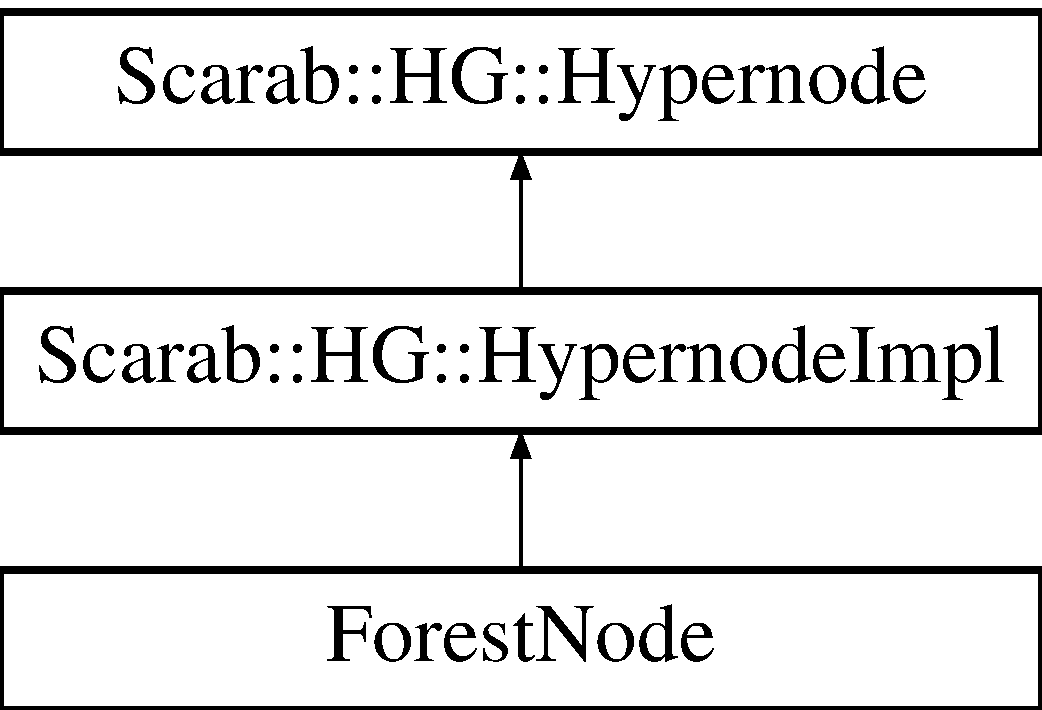
\includegraphics[height=3cm]{class_forest_node}
\end{center}
\end{figure}
\subsection*{Public Member Functions}
\begin{DoxyCompactItemize}
\item 
\hypertarget{class_forest_node_aeeb649eef15a82d283ae728b0a44d183}{
{\bfseries ForestNode} (const string \&label, int id, str\_\-vector $\ast$features, string word, bool is\_\-word)}
\label{class_forest_node_aeeb649eef15a82d283ae728b0a44d183}

\item 
\hypertarget{class_forest_node_ab44af8003df7af0ce93b9b904301fb92}{
bool {\bfseries is\_\-word} () const }
\label{class_forest_node_ab44af8003df7af0ce93b9b904301fb92}

\item 
\hypertarget{class_forest_node_a18c00f9aae93bc963358e488f2cce308}{
string {\bfseries word} () const }
\label{class_forest_node_a18c00f9aae93bc963358e488f2cce308}

\end{DoxyCompactItemize}


The documentation for this class was generated from the following file:\begin{DoxyCompactItemize}
\item 
transforest/Forest.h\end{DoxyCompactItemize}

\hypertarget{class_scarab_1_1_graph_1_1_graph}{
\section{Scarab::Graph::Graph Class Reference}
\label{class_scarab_1_1_graph_1_1_graph}\index{Scarab::Graph::Graph@{Scarab::Graph::Graph}}
}
\subsection*{Public Member Functions}
\begin{DoxyCompactItemize}
\item 
\hypertarget{class_scarab_1_1_graph_1_1_graph_ac753f9750341458516e06fb1437a1258}{
{\bfseries Graph} (const Nodes \&nodes, const Edges \&edges)}
\label{class_scarab_1_1_graph_1_1_graph_ac753f9750341458516e06fb1437a1258}

\item 
uint \hyperlink{class_scarab_1_1_graph_1_1_graph_afdfbdd8e5427a646707ceb22ca15d2e2}{num\_\-edges} () const 
\item 
\hypertarget{class_scarab_1_1_graph_1_1_graph_ac35877b52ec1f625ff452a4073026b26}{
uint {\bfseries num\_\-nodes} () const }
\label{class_scarab_1_1_graph_1_1_graph_ac35877b52ec1f625ff452a4073026b26}

\item 
\hypertarget{class_scarab_1_1_graph_1_1_graph_a8d0c6189ef1569626348a30e908870e4}{
const Nodes \& {\bfseries nodes} () const }
\label{class_scarab_1_1_graph_1_1_graph_a8d0c6189ef1569626348a30e908870e4}

\item 
\hypertarget{class_scarab_1_1_graph_1_1_graph_a19a63be838e64b57e46cba029e273162}{
const Edges \& {\bfseries edges} () const }
\label{class_scarab_1_1_graph_1_1_graph_a19a63be838e64b57e46cba029e273162}

\item 
\hypertarget{class_scarab_1_1_graph_1_1_graph_af226b4907b00e178a8f7bd6e972e42d2}{
const \hyperlink{class_scarab_1_1_graph_1_1_graphnode}{Graphnode} \& {\bfseries node} (uint i) const }
\label{class_scarab_1_1_graph_1_1_graph_af226b4907b00e178a8f7bd6e972e42d2}

\end{DoxyCompactItemize}


\subsection{Member Function Documentation}
\hypertarget{class_scarab_1_1_graph_1_1_graph_afdfbdd8e5427a646707ceb22ca15d2e2}{
\index{Scarab::Graph::Graph@{Scarab::Graph::Graph}!num\_\-edges@{num\_\-edges}}
\index{num\_\-edges@{num\_\-edges}!Scarab::Graph::Graph@{Scarab::Graph::Graph}}
\subsubsection[{num\_\-edges}]{\setlength{\rightskip}{0pt plus 5cm}uint Scarab::Graph::Graph::num\_\-edges () const\hspace{0.3cm}{\ttfamily  \mbox{[}inline\mbox{]}}}}
\label{class_scarab_1_1_graph_1_1_graph_afdfbdd8e5427a646707ceb22ca15d2e2}
Display the graph for debugging. 

The documentation for this class was generated from the following file:\begin{DoxyCompactItemize}
\item 
graph/Graph.h\end{DoxyCompactItemize}

\hypertarget{class_graph_decompose}{
\section{GraphDecompose Class Reference}
\label{class_graph_decompose}\index{GraphDecompose@{GraphDecompose}}
}
\subsection*{Public Member Functions}
\begin{DoxyCompactItemize}
\item 
\hypertarget{class_graph_decompose_a671b195e2a0eff48eeefcee64d40fcb1}{
void {\bfseries decompose} (const \hyperlink{class_forest_lattice}{ForestLattice} $\ast$g)}
\label{class_graph_decompose_a671b195e2a0eff48eeefcee64d40fcb1}

\item 
\hypertarget{class_graph_decompose_a8e85b51d78e6bd961bbff6d121399ba7}{
bool {\bfseries path\_\-exists} (int w1, int w2) const }
\label{class_graph_decompose_a8e85b51d78e6bd961bbff6d121399ba7}

\item 
\hypertarget{class_graph_decompose_a48e47d62512330c280ed8a89bafe3e10}{
vector$<$ int $>$ $\ast$ {\bfseries get\_\-path} (int w1, int w2) const }
\label{class_graph_decompose_a48e47d62512330c280ed8a89bafe3e10}

\end{DoxyCompactItemize}
\subsection*{Public Attributes}
\begin{DoxyCompactItemize}
\item 
\hypertarget{class_graph_decompose_afbeb52935da971f4bc27f0e80ed48d33}{
vector$<$ \hyperlink{struct_bigram}{Bigram} $>$ {\bfseries valid\_\-bigrams}}
\label{class_graph_decompose_afbeb52935da971f4bc27f0e80ed48d33}

\item 
\hypertarget{class_graph_decompose_aca254d25cf0f2d2ad0d58a5775a297a8}{
vector$<$ vector$<$ int $>$ $>$ {\bfseries forward\_\-bigrams}}
\label{class_graph_decompose_aca254d25cf0f2d2ad0d58a5775a297a8}

\item 
\hypertarget{class_graph_decompose_a2b5c495d7725ccd63c0c3d2590ebd1e1}{
vector$<$ vector$<$ int $>$ $>$ {\bfseries backward\_\-bigrams}}
\label{class_graph_decompose_a2b5c495d7725ccd63c0c3d2590ebd1e1}

\end{DoxyCompactItemize}


The documentation for this class was generated from the following files:\begin{DoxyCompactItemize}
\item 
lattice/GraphDecompose.h\item 
lattice/GraphDecompose.cpp\end{DoxyCompactItemize}

\hypertarget{class_scarab_1_1_graph_1_1_graphedge}{
\section{Scarab::Graph::Graphedge Class Reference}
\label{class_scarab_1_1_graph_1_1_graphedge}\index{Scarab::Graph::Graphedge@{Scarab::Graph::Graphedge}}
}
\subsection*{Public Member Functions}
\begin{DoxyCompactItemize}
\item 
\hypertarget{class_scarab_1_1_graph_1_1_graphedge_aea165d2e0b46a46180f5e684df52abdf}{
{\bfseries Graphedge} (uint id, const \hyperlink{class_scarab_1_1_graph_1_1_graphnode}{Graphnode} \&from, const \hyperlink{class_scarab_1_1_graph_1_1_graphnode}{Graphnode} \&to)}
\label{class_scarab_1_1_graph_1_1_graphedge_aea165d2e0b46a46180f5e684df52abdf}

\item 
uint \hyperlink{class_scarab_1_1_graph_1_1_graphedge_af4e2b922eb0db014aa6af45ef911e47c}{id} () const 
\item 
\hypertarget{class_scarab_1_1_graph_1_1_graphedge_a10760ab9034b358f9bd4aa28c44117d5}{
\hyperlink{class_scarab_1_1_graph_1_1_graphnode}{Node} {\bfseries from\_\-node} () const }
\label{class_scarab_1_1_graph_1_1_graphedge_a10760ab9034b358f9bd4aa28c44117d5}

\item 
\hypertarget{class_scarab_1_1_graph_1_1_graphedge_ae5b1fccfa8a11847b8be2a27690243f0}{
\hyperlink{class_scarab_1_1_graph_1_1_graphnode}{Node} {\bfseries to\_\-node} () const }
\label{class_scarab_1_1_graph_1_1_graphedge_ae5b1fccfa8a11847b8be2a27690243f0}

\end{DoxyCompactItemize}


\subsection{Member Function Documentation}
\hypertarget{class_scarab_1_1_graph_1_1_graphedge_af4e2b922eb0db014aa6af45ef911e47c}{
\index{Scarab::Graph::Graphedge@{Scarab::Graph::Graphedge}!id@{id}}
\index{id@{id}!Scarab::Graph::Graphedge@{Scarab::Graph::Graphedge}}
\subsubsection[{id}]{\setlength{\rightskip}{0pt plus 5cm}uint Scarab::Graph::Graphedge::id () const\hspace{0.3cm}{\ttfamily  \mbox{[}inline\mbox{]}}}}
\label{class_scarab_1_1_graph_1_1_graphedge_af4e2b922eb0db014aa6af45ef911e47c}
Get edge id

\begin{DoxyReturn}{Returns}
The id of this edge in a fixed graph 
\end{DoxyReturn}


The documentation for this class was generated from the following file:\begin{DoxyCompactItemize}
\item 
graph/Graph.h\end{DoxyCompactItemize}

\hypertarget{class_scarab_1_1_graph_1_1_graphnode}{
\section{Scarab::Graph::Graphnode Class Reference}
\label{class_scarab_1_1_graph_1_1_graphnode}\index{Scarab::Graph::Graphnode@{Scarab::Graph::Graphnode}}
}
\subsection*{Public Member Functions}
\begin{DoxyCompactItemize}
\item 
\hypertarget{class_scarab_1_1_graph_1_1_graphnode_adce1b3b5b83d8fca4952f244bd093b9f}{
{\bfseries Graphnode} (uint id)}
\label{class_scarab_1_1_graph_1_1_graphnode_adce1b3b5b83d8fca4952f244bd093b9f}

\item 
uint \hyperlink{class_scarab_1_1_graph_1_1_graphnode_a74eaaed5d31a0a2c0445f3de0859148f}{id} () const 
\item 
uint \hyperlink{class_scarab_1_1_graph_1_1_graphnode_a78229cc45113d24f1373a50a13bc7be4}{num\_\-edges} () const 
\item 
\hypertarget{class_scarab_1_1_graph_1_1_graphnode_a717294ebbae2d29e9f97633407dae4ce}{
uint {\bfseries num\_\-in\_\-edges} () const }
\label{class_scarab_1_1_graph_1_1_graphnode_a717294ebbae2d29e9f97633407dae4ce}

\item 
const Edges \& \hyperlink{class_scarab_1_1_graph_1_1_graphnode_a4ffd990052c812242cbdeeae7b0e1104}{edges} () const 
\item 
\hypertarget{class_scarab_1_1_graph_1_1_graphnode_a001915a0fd7a6d4b06886f7865fc5189}{
const Edges \& {\bfseries in\_\-edges} () const }
\label{class_scarab_1_1_graph_1_1_graphnode_a001915a0fd7a6d4b06886f7865fc5189}

\item 
\hypertarget{class_scarab_1_1_graph_1_1_graphnode_ae37c75fd607395376ade1cda5294e2a4}{
void {\bfseries set\_\-edges} (Edges edges)}
\label{class_scarab_1_1_graph_1_1_graphnode_ae37c75fd607395376ade1cda5294e2a4}

\item 
\hypertarget{class_scarab_1_1_graph_1_1_graphnode_a22e722e5bcd49dcfa643304d631416dc}{
void {\bfseries add\_\-edge} (\hyperlink{class_scarab_1_1_graph_1_1_graphedge}{Edge} edge)}
\label{class_scarab_1_1_graph_1_1_graphnode_a22e722e5bcd49dcfa643304d631416dc}

\item 
\hypertarget{class_scarab_1_1_graph_1_1_graphnode_a092b914639364b7b9168c84e3e556cea}{
void {\bfseries add\_\-in\_\-edge} (\hyperlink{class_scarab_1_1_graph_1_1_graphedge}{Edge} edge)}
\label{class_scarab_1_1_graph_1_1_graphnode_a092b914639364b7b9168c84e3e556cea}

\item 
\hypertarget{class_scarab_1_1_graph_1_1_graphnode_a7ec0926462b47496b1158f16b87e69ca}{
void {\bfseries set\_\-label} (string lab)}
\label{class_scarab_1_1_graph_1_1_graphnode_a7ec0926462b47496b1158f16b87e69ca}

\end{DoxyCompactItemize}


\subsection{Member Function Documentation}
\hypertarget{class_scarab_1_1_graph_1_1_graphnode_a4ffd990052c812242cbdeeae7b0e1104}{
\index{Scarab::Graph::Graphnode@{Scarab::Graph::Graphnode}!edges@{edges}}
\index{edges@{edges}!Scarab::Graph::Graphnode@{Scarab::Graph::Graphnode}}
\subsubsection[{edges}]{\setlength{\rightskip}{0pt plus 5cm}const Edges\& Scarab::Graph::Graphnode::edges () const\hspace{0.3cm}{\ttfamily  \mbox{[}inline\mbox{]}}}}
\label{class_scarab_1_1_graph_1_1_graphnode_a4ffd990052c812242cbdeeae7b0e1104}
Get all edges with this node as head.

Treat this as a const iterator. \begin{DoxyReturn}{Returns}
Const iterator to edges. 
\end{DoxyReturn}
\hypertarget{class_scarab_1_1_graph_1_1_graphnode_a74eaaed5d31a0a2c0445f3de0859148f}{
\index{Scarab::Graph::Graphnode@{Scarab::Graph::Graphnode}!id@{id}}
\index{id@{id}!Scarab::Graph::Graphnode@{Scarab::Graph::Graphnode}}
\subsubsection[{id}]{\setlength{\rightskip}{0pt plus 5cm}uint Scarab::Graph::Graphnode::id () const\hspace{0.3cm}{\ttfamily  \mbox{[}inline\mbox{]}}}}
\label{class_scarab_1_1_graph_1_1_graphnode_a74eaaed5d31a0a2c0445f3de0859148f}
The unique identifier of the \hyperlink{class_scarab_1_1_graph_1_1_graphnode}{Graphnode} \begin{Desc}
\item[\hyperlink{deprecated__deprecated000001}{Deprecated}]\end{Desc}
\begin{DoxyReturn}{Returns}
The number 
\end{DoxyReturn}
\hypertarget{class_scarab_1_1_graph_1_1_graphnode_a78229cc45113d24f1373a50a13bc7be4}{
\index{Scarab::Graph::Graphnode@{Scarab::Graph::Graphnode}!num\_\-edges@{num\_\-edges}}
\index{num\_\-edges@{num\_\-edges}!Scarab::Graph::Graphnode@{Scarab::Graph::Graphnode}}
\subsubsection[{num\_\-edges}]{\setlength{\rightskip}{0pt plus 5cm}uint Scarab::Graph::Graphnode::num\_\-edges () const\hspace{0.3cm}{\ttfamily  \mbox{[}inline\mbox{]}}}}
\label{class_scarab_1_1_graph_1_1_graphnode_a78229cc45113d24f1373a50a13bc7be4}
Get the number of edges connected to this node \begin{Desc}
\item[\hyperlink{deprecated__deprecated000002}{Deprecated}]\end{Desc}
\begin{DoxyReturn}{Returns}
The number 
\end{DoxyReturn}


The documentation for this class was generated from the following file:\begin{DoxyCompactItemize}
\item 
graph/Graph.h\end{DoxyCompactItemize}

\hypertarget{class_graph_proto_interface}{
\section{GraphProtoInterface Class Reference}
\label{class_graph_proto_interface}\index{GraphProtoInterface@{GraphProtoInterface}}
}
Inheritance diagram for GraphProtoInterface:\begin{figure}[H]
\begin{center}
\leavevmode
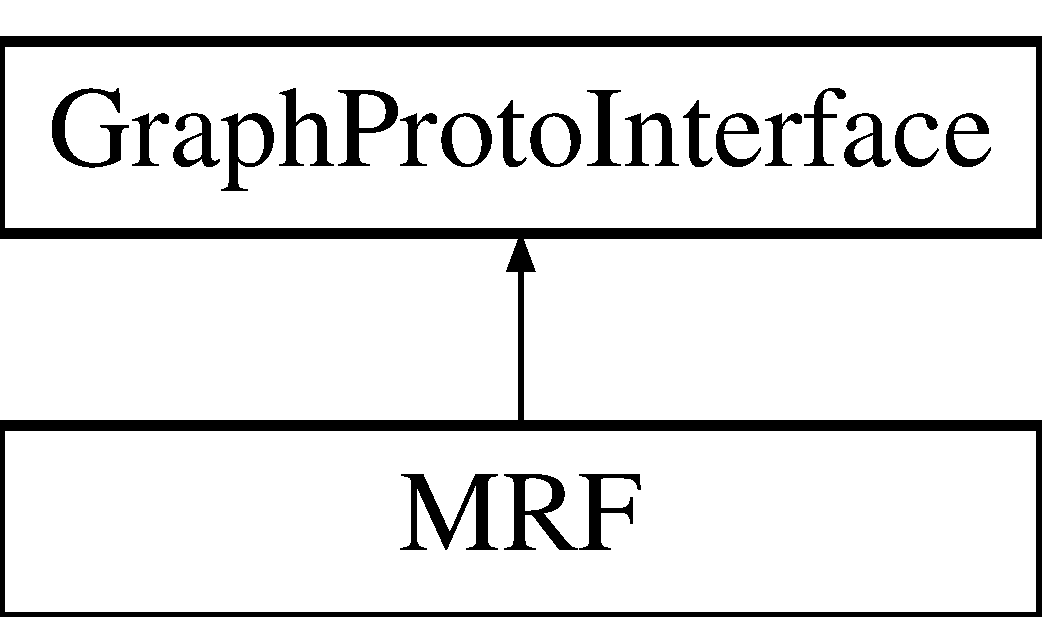
\includegraphics[height=2cm]{class_graph_proto_interface}
\end{center}
\end{figure}
\subsection*{Public Member Functions}
\begin{DoxyCompactItemize}
\item 
\hypertarget{class_graph_proto_interface_a4845501ec86ea627ce484cd78162c84c}{
void {\bfseries build\_\-from\_\-file} (const char $\ast$file\_\-name)}
\label{class_graph_proto_interface_a4845501ec86ea627ce484cd78162c84c}

\item 
\hypertarget{class_graph_proto_interface_a0dbd0905dbab167b9293d0ef32409af3}{
virtual void {\bfseries process\_\-node} (graph::Graph\_\-Node, \hyperlink{class_scarab_1_1_graph_1_1_graphnode}{Graphnode} $\ast$)=0}
\label{class_graph_proto_interface_a0dbd0905dbab167b9293d0ef32409af3}

\item 
\hypertarget{class_graph_proto_interface_a3178c5f1eff8ed61d2512af8522cc550}{
virtual void {\bfseries process\_\-edge} (graph::Graph\_\-Edge, \hyperlink{class_scarab_1_1_graph_1_1_graphedge}{Graphedge} $\ast$)=0}
\label{class_graph_proto_interface_a3178c5f1eff8ed61d2512af8522cc550}

\item 
\hypertarget{class_graph_proto_interface_a8b3125379c7b2bbf832b6b955496b76e}{
virtual void {\bfseries set\_\-up} (graph::Graph, int, int)}
\label{class_graph_proto_interface_a8b3125379c7b2bbf832b6b955496b76e}

\item 
\hypertarget{class_graph_proto_interface_a920e88785192db805206c875a8a3feed}{
const \hyperlink{class_scarab_1_1_graph_1_1_graph}{Graph} \& {\bfseries graph} () const }
\label{class_graph_proto_interface_a920e88785192db805206c875a8a3feed}

\end{DoxyCompactItemize}
\subsection*{Public Attributes}
\begin{DoxyCompactItemize}
\item 
\hypertarget{class_graph_proto_interface_a8e262de0a3f65eaa20e5c528363bbb2a}{
\hyperlink{class_scarab_1_1_graph_1_1_graph}{Graph} $\ast$ {\bfseries \_\-graph}}
\label{class_graph_proto_interface_a8e262de0a3f65eaa20e5c528363bbb2a}

\end{DoxyCompactItemize}


The documentation for this class was generated from the following files:\begin{DoxyCompactItemize}
\item 
graph/GraphProtoInterface.h\item 
graph/GraphProtoInterface.cpp\end{DoxyCompactItemize}

\hypertarget{class_hard_constraints}{
\section{HardConstraints Class Reference}
\label{class_hard_constraints}\index{HardConstraints@{HardConstraints}}
}
\subsection*{Public Member Functions}
\begin{DoxyCompactItemize}
\item 
\hypertarget{class_hard_constraints_ad457a78e966e6ce3d71bfb3401b0300b}{
void {\bfseries read\_\-from\_\-file} (string file\_\-name)}
\label{class_hard_constraints_ad457a78e966e6ce3d71bfb3401b0300b}

\item 
\hypertarget{class_hard_constraints_a923f4ddd8b164d924147c22f054a9c7e}{
GRBLinExpr {\bfseries make\_\-lin\_\-expr} (const vector$<$ \hyperlink{struct_scarab_1_1_h_g_1_1_dep_parser_l_p}{DepParserLP} $\ast$ $>$ \&lp\_\-vars, const \hyperlink{struct_possible_dep}{PossibleDep} \&dep)}
\label{class_hard_constraints_a923f4ddd8b164d924147c22f054a9c7e}

\item 
\hypertarget{class_hard_constraints_a0945fb67209be1cc95b31522d96e51cc}{
void {\bfseries show\_\-results} ()}
\label{class_hard_constraints_a0945fb67209be1cc95b31522d96e51cc}

\item 
\hypertarget{class_hard_constraints_a71ae98e67f5e5d3035aff1c2ef941a92}{
void {\bfseries add\_\-to\_\-lp} (const vector$<$ \hyperlink{struct_scarab_1_1_h_g_1_1_dep_parser_l_p}{DepParserLP} $\ast$ $>$ \&lp\_\-vars, GRBModel \&model)}
\label{class_hard_constraints_a71ae98e67f5e5d3035aff1c2ef941a92}

\end{DoxyCompactItemize}
\subsection*{Public Attributes}
\begin{DoxyCompactItemize}
\item 
\hypertarget{class_hard_constraints_ae0305e95d8065eb186ccae220b8e16f4}{
vector$<$ vector$<$ \hyperlink{struct_possible_dep}{PossibleDep} $>$ $>$ {\bfseries \_\-constraint\_\-struct}}
\label{class_hard_constraints_ae0305e95d8065eb186ccae220b8e16f4}

\item 
\hypertarget{class_hard_constraints_a6b370ae5376bf283115092ab4bd33743}{
vector$<$ GRBVar $>$ {\bfseries group\_\-used}}
\label{class_hard_constraints_a6b370ae5376bf283115092ab4bd33743}

\end{DoxyCompactItemize}


The documentation for this class was generated from the following file:\begin{DoxyCompactItemize}
\item 
lp/HardConstraints.h\end{DoxyCompactItemize}

\hypertarget{class_hard_pos_constraints_l_p}{
\section{HardPosConstraintsLP Class Reference}
\label{class_hard_pos_constraints_l_p}\index{HardPosConstraintsLP@{HardPosConstraintsLP}}
}
\subsection*{Public Member Functions}
\begin{DoxyCompactItemize}
\item 
\hypertarget{class_hard_pos_constraints_l_p_a2979e37eb163b00f48a38ee8fccd1a64}{
{\bfseries HardPosConstraintsLP} (const \hyperlink{class_tag_constraints}{TagConstraints} \&constraints, double penalty)}
\label{class_hard_pos_constraints_l_p_a2979e37eb163b00f48a38ee8fccd1a64}

\item 
\hypertarget{class_hard_pos_constraints_l_p_aa841ffcec001c0ee31714d0d39027c26}{
GRBLinExpr {\bfseries make\_\-lin\_\-expr} (const vector$<$ \hyperlink{struct_scarab_1_1_h_g_1_1_tag_l_p}{TagLP} $\ast$ $>$ \&lp\_\-vars, const \hyperlink{struct_possible_tag}{PossibleTag} \&tag, POS restricted\_\-to)}
\label{class_hard_pos_constraints_l_p_aa841ffcec001c0ee31714d0d39027c26}

\item 
\hypertarget{class_hard_pos_constraints_l_p_a7a7bb0c41351c9de3130045f0013c67b}{
void {\bfseries add\_\-to\_\-lp} (const vector$<$ \hyperlink{struct_scarab_1_1_h_g_1_1_tag_l_p}{TagLP} $\ast$ $>$ \&lp\_\-vars, GRBModel \&model)}
\label{class_hard_pos_constraints_l_p_a7a7bb0c41351c9de3130045f0013c67b}

\item 
\hypertarget{class_hard_pos_constraints_l_p_a4307bcde1a701018736de348a718262b}{
void {\bfseries show\_\-results} ()}
\label{class_hard_pos_constraints_l_p_a4307bcde1a701018736de348a718262b}

\end{DoxyCompactItemize}
\subsection*{Public Attributes}
\begin{DoxyCompactItemize}
\item 
\hypertarget{class_hard_pos_constraints_l_p_a16ba65107e587a8cb43cc10949b0ebcf}{
vector$<$ vector$<$ GRBVar $>$ $>$ {\bfseries group\_\-used}}
\label{class_hard_pos_constraints_l_p_a16ba65107e587a8cb43cc10949b0ebcf}

\item 
\hypertarget{class_hard_pos_constraints_l_p_ad3b98e9e78140b02098420c674fcbaab}{
vector$<$ vector$<$ vector$<$ GRBVar $>$ $>$ $>$ {\bfseries slacks\_\-pos}}
\label{class_hard_pos_constraints_l_p_ad3b98e9e78140b02098420c674fcbaab}

\item 
\hypertarget{class_hard_pos_constraints_l_p_ac758c0971f82ef892f7f708db15bf472}{
vector$<$ vector$<$ vector$<$ GRBVar $>$ $>$ $>$ {\bfseries slacks\_\-neg}}
\label{class_hard_pos_constraints_l_p_ac758c0971f82ef892f7f708db15bf472}

\item 
\hypertarget{class_hard_pos_constraints_l_p_aa5c46efababe8dd5282a71ceb233c548}{
set$<$ int $>$ {\bfseries groups}}
\label{class_hard_pos_constraints_l_p_aa5c46efababe8dd5282a71ceb233c548}

\end{DoxyCompactItemize}


The documentation for this class was generated from the following file:\begin{DoxyCompactItemize}
\item 
lp/HardPosConstraints.h\end{DoxyCompactItemize}

\hypertarget{class_scarab_1_1_h_g_1_1_heuristic}{
\section{Scarab::HG::Heuristic Class Reference}
\label{class_scarab_1_1_h_g_1_1_heuristic}\index{Scarab::HG::Heuristic@{Scarab::HG::Heuristic}}
}
Inheritance diagram for Scarab::HG::Heuristic:\begin{figure}[H]
\begin{center}
\leavevmode
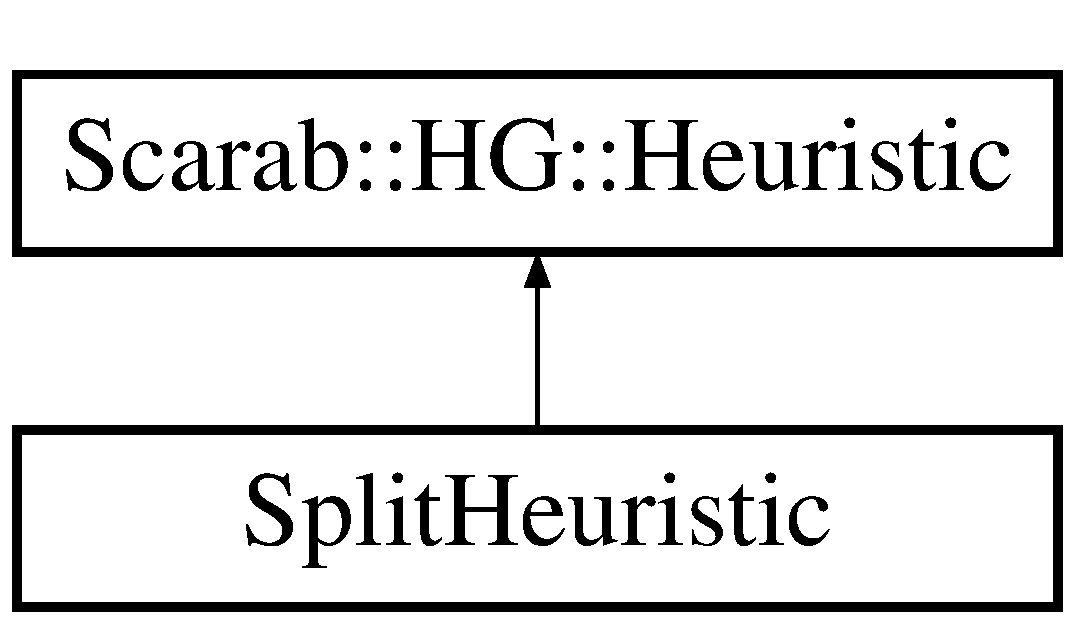
\includegraphics[height=2cm]{class_scarab_1_1_h_g_1_1_heuristic}
\end{center}
\end{figure}
\subsection*{Public Member Functions}
\begin{DoxyCompactItemize}
\item 
\hypertarget{class_scarab_1_1_h_g_1_1_heuristic_afad5a99d38b6783521e4c670d3edcf0a}{
virtual bool {\bfseries has\_\-value} (const \hyperlink{struct_scarab_1_1_h_g_1_1_location}{Location} \&loc, const \hyperlink{struct_scarab_1_1_h_g_1_1_hypothesis}{Hypothesis} \&hyp) const =0}
\label{class_scarab_1_1_h_g_1_1_heuristic_afad5a99d38b6783521e4c670d3edcf0a}

\item 
\hypertarget{class_scarab_1_1_h_g_1_1_heuristic_aca6b5924257b35be9e65058062fdc0d5}{
virtual double {\bfseries get\_\-value} (const \hyperlink{struct_scarab_1_1_h_g_1_1_location}{Location} \&loc, const \hyperlink{struct_scarab_1_1_h_g_1_1_hypothesis}{Hypothesis} \&hyp) const =0}
\label{class_scarab_1_1_h_g_1_1_heuristic_aca6b5924257b35be9e65058062fdc0d5}

\end{DoxyCompactItemize}


The documentation for this class was generated from the following file:\begin{DoxyCompactItemize}
\item 
hypergraph/AStar.h\end{DoxyCompactItemize}

\hypertarget{class_scarab_1_1_h_g_1_1_h_graph}{
\section{Scarab::HG::HGraph Class Reference}
\label{class_scarab_1_1_h_g_1_1_h_graph}\index{Scarab::HG::HGraph@{Scarab::HG::HGraph}}
}
Inheritance diagram for Scarab::HG::HGraph:\begin{figure}[H]
\begin{center}
\leavevmode
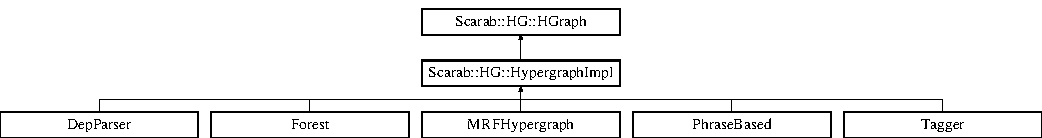
\includegraphics[height=1.85635cm]{class_scarab_1_1_h_g_1_1_h_graph}
\end{center}
\end{figure}
\subsection*{Public Member Functions}
\begin{DoxyCompactItemize}
\item 
virtual void \hyperlink{class_scarab_1_1_h_g_1_1_h_graph_ab5aa11c932b28864b56f28e0babbc1c1}{print} () const =0
\item 
virtual const \hyperlink{class_scarab_1_1_h_g_1_1_hypernode}{Hypernode} \& \hyperlink{class_scarab_1_1_h_g_1_1_h_graph_a5ede392b158e41dd7e95ded1c4b0b5d6}{root} () const =0
\item 
\hypertarget{class_scarab_1_1_h_g_1_1_h_graph_a8309003db80be5bdbe4bb64f98a78ea8}{
virtual unsigned int {\bfseries num\_\-edges} () const =0}
\label{class_scarab_1_1_h_g_1_1_h_graph_a8309003db80be5bdbe4bb64f98a78ea8}

\item 
\hypertarget{class_scarab_1_1_h_g_1_1_h_graph_a6f4d37ef034cb38aa09c702b80a6e4f7}{
virtual unsigned int {\bfseries num\_\-nodes} () const =0}
\label{class_scarab_1_1_h_g_1_1_h_graph_a6f4d37ef034cb38aa09c702b80a6e4f7}

\item 
\hypertarget{class_scarab_1_1_h_g_1_1_h_graph_acad57dd952956b1a1a4367bba0e9383b}{
virtual const \hyperlink{class_scarab_1_1_h_g_1_1_hypernode}{Hypernode} \& {\bfseries get\_\-node} (unsigned int i) const =0}
\label{class_scarab_1_1_h_g_1_1_h_graph_acad57dd952956b1a1a4367bba0e9383b}

\item 
\hypertarget{class_scarab_1_1_h_g_1_1_h_graph_aa599b296ae01affc9606f519e4e44e9e}{
virtual const \hyperlink{class_scarab_1_1_h_g_1_1_hyperedge}{Hyperedge} \& {\bfseries get\_\-edge} (unsigned int i) const =0}
\label{class_scarab_1_1_h_g_1_1_h_graph_aa599b296ae01affc9606f519e4e44e9e}

\item 
virtual const vector$<$ \hyperlink{class_scarab_1_1_h_g_1_1_hypernode}{Hypernode} $\ast$ $>$ \& \hyperlink{class_scarab_1_1_h_g_1_1_h_graph_a74d893fba015520774f71f02a46bb6ca}{nodes} () const =0
\item 
virtual const vector$<$ \hyperlink{class_scarab_1_1_h_g_1_1_hyperedge}{Hyperedge} $\ast$ $>$ \& \hyperlink{class_scarab_1_1_h_g_1_1_h_graph_a57328729f90cc4152ca79ff15ecdd4bb}{edges} () const =0
\end{DoxyCompactItemize}


\subsection{Member Function Documentation}
\hypertarget{class_scarab_1_1_h_g_1_1_h_graph_a57328729f90cc4152ca79ff15ecdd4bb}{
\index{Scarab::HG::HGraph@{Scarab::HG::HGraph}!edges@{edges}}
\index{edges@{edges}!Scarab::HG::HGraph@{Scarab::HG::HGraph}}
\subsubsection[{edges}]{\setlength{\rightskip}{0pt plus 5cm}virtual const vector$<${\bf Hyperedge}$\ast$$>$\& Scarab::HG::HGraph::edges () const\hspace{0.3cm}{\ttfamily  \mbox{[}pure virtual\mbox{]}}}}
\label{class_scarab_1_1_h_g_1_1_h_graph_a57328729f90cc4152ca79ff15ecdd4bb}
Get all hyperedges in the hypergraph. (Assume unordered) WARNING: Treat this as a const iterator. \begin{DoxyReturn}{Returns}
Const iterator to edges in hypergraph . 
\end{DoxyReturn}


Implemented in \hyperlink{class_scarab_1_1_h_g_1_1_hypergraph_impl_a0c8373e545fe59b0cb7036b4751508e1}{Scarab::HG::HypergraphImpl}.

\hypertarget{class_scarab_1_1_h_g_1_1_h_graph_a74d893fba015520774f71f02a46bb6ca}{
\index{Scarab::HG::HGraph@{Scarab::HG::HGraph}!nodes@{nodes}}
\index{nodes@{nodes}!Scarab::HG::HGraph@{Scarab::HG::HGraph}}
\subsubsection[{nodes}]{\setlength{\rightskip}{0pt plus 5cm}virtual const vector$<${\bf Hypernode}$\ast$ $>$\& Scarab::HG::HGraph::nodes () const\hspace{0.3cm}{\ttfamily  \mbox{[}pure virtual\mbox{]}}}}
\label{class_scarab_1_1_h_g_1_1_h_graph_a74d893fba015520774f71f02a46bb6ca}
Get all hypernodes in the hypergraph. (Assume unordered) WARNING: Treat this as a const iterator. \begin{DoxyReturn}{Returns}
Const iterator to hypernodes in hypergraph . 
\end{DoxyReturn}


Implemented in \hyperlink{class_scarab_1_1_h_g_1_1_hypergraph_impl_a9aef2881b489c86d4d83e996a70f8141}{Scarab::HG::HypergraphImpl}.

\hypertarget{class_scarab_1_1_h_g_1_1_h_graph_ab5aa11c932b28864b56f28e0babbc1c1}{
\index{Scarab::HG::HGraph@{Scarab::HG::HGraph}!print@{print}}
\index{print@{print}!Scarab::HG::HGraph@{Scarab::HG::HGraph}}
\subsubsection[{print}]{\setlength{\rightskip}{0pt plus 5cm}virtual void Scarab::HG::HGraph::print () const\hspace{0.3cm}{\ttfamily  \mbox{[}pure virtual\mbox{]}}}}
\label{class_scarab_1_1_h_g_1_1_h_graph_ab5aa11c932b28864b56f28e0babbc1c1}
Display the hypergraph for debugging. 

Implemented in \hyperlink{class_m_r_f_hypergraph_aaac6b68c3ece41ddd1f8107e961879bc}{MRFHypergraph}, \hyperlink{class_dep_parser_a9aebbbde821bad423b6c01cc12f02a2c}{DepParser}, \hyperlink{class_phrase_based_aafc2997b58b3698fed7cb5a1f6f269c6}{PhraseBased}, \hyperlink{class_tagger_a4ebe0aebd7c0392970b401a5a6c6cd72}{Tagger}, and \hyperlink{class_forest_a621a1a65d0f877bb33b15c79f9e24c4d}{Forest}.

\hypertarget{class_scarab_1_1_h_g_1_1_h_graph_a5ede392b158e41dd7e95ded1c4b0b5d6}{
\index{Scarab::HG::HGraph@{Scarab::HG::HGraph}!root@{root}}
\index{root@{root}!Scarab::HG::HGraph@{Scarab::HG::HGraph}}
\subsubsection[{root}]{\setlength{\rightskip}{0pt plus 5cm}virtual const {\bf Hypernode}\& Scarab::HG::HGraph::root () const\hspace{0.3cm}{\ttfamily  \mbox{[}pure virtual\mbox{]}}}}
\label{class_scarab_1_1_h_g_1_1_h_graph_a5ede392b158e41dd7e95ded1c4b0b5d6}
Get the root of the hypergraph

\begin{DoxyReturn}{Returns}
\hyperlink{class_scarab_1_1_h_g_1_1_hypernode}{Hypernode} at root 
\end{DoxyReturn}


Implemented in \hyperlink{class_scarab_1_1_h_g_1_1_hypergraph_impl_a31172009b97d179f6b1199f191197a32}{Scarab::HG::HypergraphImpl}.



The documentation for this class was generated from the following file:\begin{DoxyCompactItemize}
\item 
hypergraph/Hypergraph.h\end{DoxyCompactItemize}

\hypertarget{struct_hyp}{
\section{Hyp Struct Reference}
\label{struct_hyp}\index{Hyp@{Hyp}}
}
\subsection*{Public Member Functions}
\begin{DoxyCompactItemize}
\item 
\hypertarget{struct_hyp_a5fba7860265cf935133e4c0c73fec090}{
{\bfseries Hyp} (double score\_\-in, Sig sig\_\-in, vector$<$ int $>$ full\_\-der)}
\label{struct_hyp_a5fba7860265cf935133e4c0c73fec090}

\item 
\hypertarget{struct_hyp_a547883a1aa9a7573d328d0f6b385dca8}{
bool {\bfseries operator$<$} (const \hyperlink{struct_hyp}{Hyp} \&other) const }
\label{struct_hyp_a547883a1aa9a7573d328d0f6b385dca8}

\end{DoxyCompactItemize}
\subsection*{Public Attributes}
\begin{DoxyCompactItemize}
\item 
\hypertarget{struct_hyp_a7d24c5a317140b8050dc57255bb7922a}{
double {\bfseries score}}
\label{struct_hyp_a7d24c5a317140b8050dc57255bb7922a}

\item 
\hypertarget{struct_hyp_a4aa96a03dc6b82416074985e0ecd39c3}{
Sig {\bfseries sig}}
\label{struct_hyp_a4aa96a03dc6b82416074985e0ecd39c3}

\item 
\hypertarget{struct_hyp_a076825f81d94a1f2b20bb5141eb9f4c7}{
vector$<$ int $>$ {\bfseries full\_\-derivation}}
\label{struct_hyp_a076825f81d94a1f2b20bb5141eb9f4c7}

\end{DoxyCompactItemize}


The documentation for this struct was generated from the following file:\begin{DoxyCompactItemize}
\item 
hypergraph/CubePruning.h\end{DoxyCompactItemize}

\hypertarget{class_scarab_1_1_h_g_1_1_hyperedge}{
\section{Scarab::HG::Hyperedge Class Reference}
\label{class_scarab_1_1_h_g_1_1_hyperedge}\index{Scarab::HG::Hyperedge@{Scarab::HG::Hyperedge}}
}
Inheritance diagram for Scarab::HG::Hyperedge:\begin{figure}[H]
\begin{center}
\leavevmode
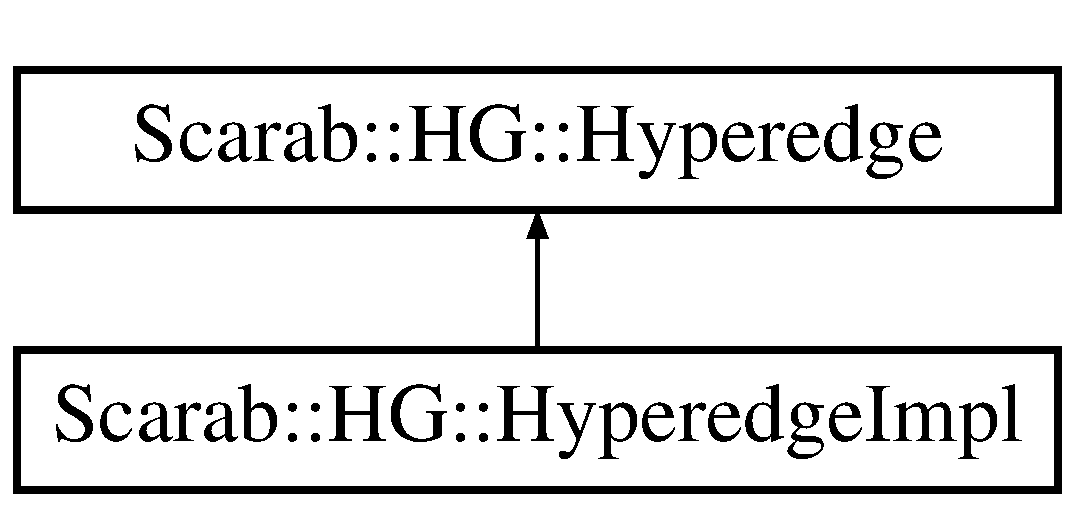
\includegraphics[height=2cm]{class_scarab_1_1_h_g_1_1_hyperedge}
\end{center}
\end{figure}
\subsection*{Public Member Functions}
\begin{DoxyCompactItemize}
\item 
virtual unsigned int \hyperlink{class_scarab_1_1_h_g_1_1_hyperedge_af824beb7107253a7545b35992c17e057}{id} () const =0
\item 
\hypertarget{class_scarab_1_1_h_g_1_1_hyperedge_a8442c017fcee87c1f865b2254b49900f}{
virtual string {\bfseries label} () const =0}
\label{class_scarab_1_1_h_g_1_1_hyperedge_a8442c017fcee87c1f865b2254b49900f}

\item 
virtual const \hyperlink{class_scarab_1_1_h_g_1_1_hypernode}{Hypernode} \& \hyperlink{class_scarab_1_1_h_g_1_1_hyperedge_a9ec8cf9ea7b5f762f359a6f9f1c038da}{tail\_\-node} (unsigned int i) const =0
\item 
virtual unsigned int \hyperlink{class_scarab_1_1_h_g_1_1_hyperedge_a799d8d98242c129d7eee178bdf1fb535}{num\_\-nodes} () const =0
\item 
virtual const svector$<$ int, double $>$ \& \hyperlink{class_scarab_1_1_h_g_1_1_hyperedge_a0d201ddb955631aadee4c15cc8e709f8}{fvector} () const =0
\item 
virtual const \hyperlink{class_scarab_1_1_h_g_1_1_hypernode}{Hypernode} \& \hyperlink{class_scarab_1_1_h_g_1_1_hyperedge_a6043de341070c103d811f5286193dd46}{head\_\-node} () const =0
\item 
virtual const vector$<$ \hyperlink{class_scarab_1_1_h_g_1_1_hypernode}{Hypernode} $\ast$ $>$ \& \hyperlink{class_scarab_1_1_h_g_1_1_hyperedge_abac6d27691186608aa12949de6e1c283}{tail\_\-nodes} () const =0
\end{DoxyCompactItemize}


\subsection{Member Function Documentation}
\hypertarget{class_scarab_1_1_h_g_1_1_hyperedge_a0d201ddb955631aadee4c15cc8e709f8}{
\index{Scarab::HG::Hyperedge@{Scarab::HG::Hyperedge}!fvector@{fvector}}
\index{fvector@{fvector}!Scarab::HG::Hyperedge@{Scarab::HG::Hyperedge}}
\subsubsection[{fvector}]{\setlength{\rightskip}{0pt plus 5cm}virtual const svector$<$int, double$>$\& Scarab::HG::Hyperedge::fvector () const\hspace{0.3cm}{\ttfamily  \mbox{[}pure virtual\mbox{]}}}}
\label{class_scarab_1_1_h_g_1_1_hyperedge_a0d201ddb955631aadee4c15cc8e709f8}
The feature vector associated with this node. TODO: remove this from the representation \begin{Desc}
\item[\hyperlink{deprecated__deprecated000005}{Deprecated}]\end{Desc}
\begin{DoxyReturn}{Returns}
Feature vector 
\end{DoxyReturn}


Implemented in \hyperlink{class_scarab_1_1_h_g_1_1_hyperedge_impl_a359446c285164a93995bb87e6ea74882}{Scarab::HG::HyperedgeImpl}.

\hypertarget{class_scarab_1_1_h_g_1_1_hyperedge_a6043de341070c103d811f5286193dd46}{
\index{Scarab::HG::Hyperedge@{Scarab::HG::Hyperedge}!head\_\-node@{head\_\-node}}
\index{head\_\-node@{head\_\-node}!Scarab::HG::Hyperedge@{Scarab::HG::Hyperedge}}
\subsubsection[{head\_\-node}]{\setlength{\rightskip}{0pt plus 5cm}virtual const {\bf Hypernode}\& Scarab::HG::Hyperedge::head\_\-node () const\hspace{0.3cm}{\ttfamily  \mbox{[}pure virtual\mbox{]}}}}
\label{class_scarab_1_1_h_g_1_1_hyperedge_a6043de341070c103d811f5286193dd46}
Get the node at the head of this hyperedge

\begin{DoxyReturn}{Returns}
Head node 
\end{DoxyReturn}


Implemented in \hyperlink{class_scarab_1_1_h_g_1_1_hyperedge_impl_ae194bfc8ecac2a12791fa36c1c2c62a7}{Scarab::HG::HyperedgeImpl}.

\hypertarget{class_scarab_1_1_h_g_1_1_hyperedge_af824beb7107253a7545b35992c17e057}{
\index{Scarab::HG::Hyperedge@{Scarab::HG::Hyperedge}!id@{id}}
\index{id@{id}!Scarab::HG::Hyperedge@{Scarab::HG::Hyperedge}}
\subsubsection[{id}]{\setlength{\rightskip}{0pt plus 5cm}virtual unsigned int Scarab::HG::Hyperedge::id () const\hspace{0.3cm}{\ttfamily  \mbox{[}pure virtual\mbox{]}}}}
\label{class_scarab_1_1_h_g_1_1_hyperedge_af824beb7107253a7545b35992c17e057}
Get edge id

\begin{DoxyReturn}{Returns}
The id of this edge in a fixed hypergraph 
\end{DoxyReturn}


Implemented in \hyperlink{class_scarab_1_1_h_g_1_1_hyperedge_impl_afa81943347267781c25c4e68f7f5f547}{Scarab::HG::HyperedgeImpl}.

\hypertarget{class_scarab_1_1_h_g_1_1_hyperedge_a799d8d98242c129d7eee178bdf1fb535}{
\index{Scarab::HG::Hyperedge@{Scarab::HG::Hyperedge}!num\_\-nodes@{num\_\-nodes}}
\index{num\_\-nodes@{num\_\-nodes}!Scarab::HG::Hyperedge@{Scarab::HG::Hyperedge}}
\subsubsection[{num\_\-nodes}]{\setlength{\rightskip}{0pt plus 5cm}virtual unsigned int Scarab::HG::Hyperedge::num\_\-nodes () const\hspace{0.3cm}{\ttfamily  \mbox{[}pure virtual\mbox{]}}}}
\label{class_scarab_1_1_h_g_1_1_hyperedge_a799d8d98242c129d7eee178bdf1fb535}
The number of tail nodes in this edge. \begin{Desc}
\item[\hyperlink{deprecated__deprecated000004}{Deprecated}]\end{Desc}
\begin{DoxyReturn}{Returns}
The length 
\end{DoxyReturn}


Implemented in \hyperlink{class_scarab_1_1_h_g_1_1_hyperedge_impl_a9a5bef8789c9c7caee6f53833ea4acc7}{Scarab::HG::HyperedgeImpl}.

\hypertarget{class_scarab_1_1_h_g_1_1_hyperedge_a9ec8cf9ea7b5f762f359a6f9f1c038da}{
\index{Scarab::HG::Hyperedge@{Scarab::HG::Hyperedge}!tail\_\-node@{tail\_\-node}}
\index{tail\_\-node@{tail\_\-node}!Scarab::HG::Hyperedge@{Scarab::HG::Hyperedge}}
\subsubsection[{tail\_\-node}]{\setlength{\rightskip}{0pt plus 5cm}virtual const {\bf Hypernode}\& Scarab::HG::Hyperedge::tail\_\-node (unsigned int {\em i}) const\hspace{0.3cm}{\ttfamily  \mbox{[}pure virtual\mbox{]}}}}
\label{class_scarab_1_1_h_g_1_1_hyperedge_a9ec8cf9ea7b5f762f359a6f9f1c038da}
Get a node in this edges tail \begin{Desc}
\item[\hyperlink{deprecated__deprecated000003}{Deprecated}]\end{Desc}

\begin{DoxyParams}{Parameters}
\item[{\em i}]The node position, in tail\_\-node order\end{DoxyParams}
\begin{DoxyReturn}{Returns}
The hypernode 
\end{DoxyReturn}


Implemented in \hyperlink{class_scarab_1_1_h_g_1_1_hyperedge_impl_a7087ba121f3056eb5946d1909c4b3d58}{Scarab::HG::HyperedgeImpl}.

\hypertarget{class_scarab_1_1_h_g_1_1_hyperedge_abac6d27691186608aa12949de6e1c283}{
\index{Scarab::HG::Hyperedge@{Scarab::HG::Hyperedge}!tail\_\-nodes@{tail\_\-nodes}}
\index{tail\_\-nodes@{tail\_\-nodes}!Scarab::HG::Hyperedge@{Scarab::HG::Hyperedge}}
\subsubsection[{tail\_\-nodes}]{\setlength{\rightskip}{0pt plus 5cm}virtual const vector$<${\bf Hypernode} $\ast$$>$\& Scarab::HG::Hyperedge::tail\_\-nodes () const\hspace{0.3cm}{\ttfamily  \mbox{[}pure virtual\mbox{]}}}}
\label{class_scarab_1_1_h_g_1_1_hyperedge_abac6d27691186608aa12949de6e1c283}
Get all the nodes in the tail of the hyperedge WARNING: Treat this as a const iterator. \begin{DoxyReturn}{Returns}
Const iterator to nodes. 
\end{DoxyReturn}


Implemented in \hyperlink{class_scarab_1_1_h_g_1_1_hyperedge_impl_a3bf00c8c032397150f59e196aea5e245}{Scarab::HG::HyperedgeImpl}.



The documentation for this class was generated from the following file:\begin{DoxyCompactItemize}
\item 
hypergraph/Hypergraph.h\end{DoxyCompactItemize}

\hypertarget{class_scarab_1_1_h_g_1_1_hyperedge_impl}{
\section{Scarab::HG::HyperedgeImpl Class Reference}
\label{class_scarab_1_1_h_g_1_1_hyperedge_impl}\index{Scarab::HG::HyperedgeImpl@{Scarab::HG::HyperedgeImpl}}
}
Inheritance diagram for Scarab::HG::HyperedgeImpl:\begin{figure}[H]
\begin{center}
\leavevmode
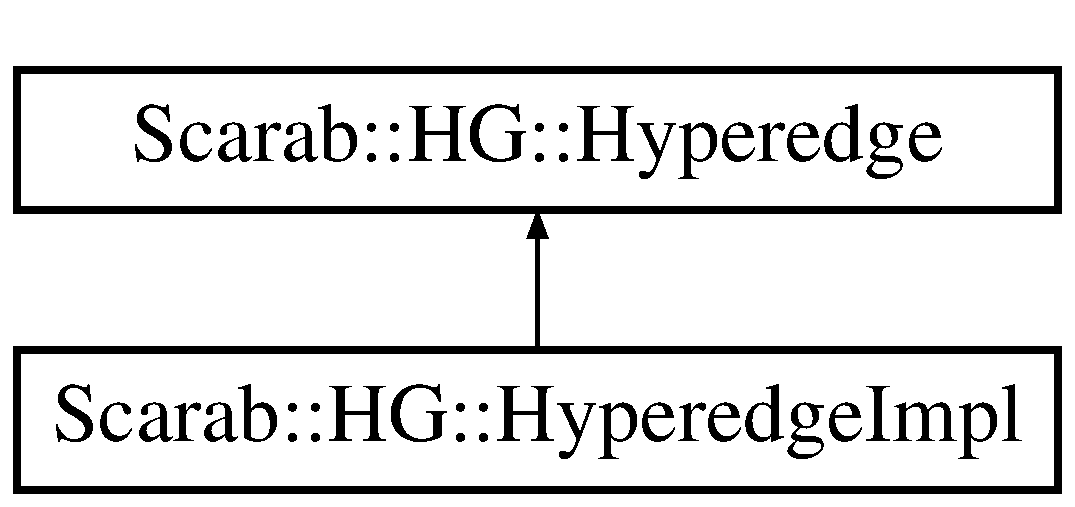
\includegraphics[height=2cm]{class_scarab_1_1_h_g_1_1_hyperedge_impl}
\end{center}
\end{figure}
\subsection*{Public Member Functions}
\begin{DoxyCompactItemize}
\item 
\hypertarget{class_scarab_1_1_h_g_1_1_hyperedge_impl_a3c141efe1be2e8ee78d45caca4711c6e}{
{\bfseries HyperedgeImpl} (const string \&label, str\_\-vector $\ast$features, int id, vector$<$ \hyperlink{class_scarab_1_1_h_g_1_1_hypernode}{Hypernode} $\ast$ $>$ tail\_\-nodes, \hyperlink{class_scarab_1_1_h_g_1_1_hypernode}{Hypernode} $\ast$head\_\-node)}
\label{class_scarab_1_1_h_g_1_1_hyperedge_impl_a3c141efe1be2e8ee78d45caca4711c6e}

\item 
const \hyperlink{class_scarab_1_1_h_g_1_1_hypernode}{Hypernode} \& \hyperlink{class_scarab_1_1_h_g_1_1_hyperedge_impl_a7087ba121f3056eb5946d1909c4b3d58}{tail\_\-node} (unsigned int i) const 
\item 
uint \hyperlink{class_scarab_1_1_h_g_1_1_hyperedge_impl_a9a5bef8789c9c7caee6f53833ea4acc7}{num\_\-nodes} () const 
\item 
const wvector \& \hyperlink{class_scarab_1_1_h_g_1_1_hyperedge_impl_a359446c285164a93995bb87e6ea74882}{fvector} () const 
\item 
const \hyperlink{class_scarab_1_1_h_g_1_1_hypernode}{Scarab::HG::Hypernode} \& \hyperlink{class_scarab_1_1_h_g_1_1_hyperedge_impl_ae194bfc8ecac2a12791fa36c1c2c62a7}{head\_\-node} () const 
\item 
const vector$<$ \hyperlink{class_scarab_1_1_h_g_1_1_hypernode}{Scarab::HG::Hypernode} $\ast$ $>$ \& \hyperlink{class_scarab_1_1_h_g_1_1_hyperedge_impl_a3bf00c8c032397150f59e196aea5e245}{tail\_\-nodes} () const 
\item 
uint \hyperlink{class_scarab_1_1_h_g_1_1_hyperedge_impl_afa81943347267781c25c4e68f7f5f547}{id} () const 
\item 
\hypertarget{class_scarab_1_1_h_g_1_1_hyperedge_impl_a8fe687c9914de37c4d91c353ba669665}{
string {\bfseries label} () const }
\label{class_scarab_1_1_h_g_1_1_hyperedge_impl_a8fe687c9914de37c4d91c353ba669665}

\item 
\hypertarget{class_scarab_1_1_h_g_1_1_hyperedge_impl_a068e4291cbcaa68a59ad64ede34f9edc}{
void {\bfseries reid} (int new\_\-id)}
\label{class_scarab_1_1_h_g_1_1_hyperedge_impl_a068e4291cbcaa68a59ad64ede34f9edc}

\end{DoxyCompactItemize}
\subsection*{Public Attributes}
\begin{DoxyCompactItemize}
\item 
\hypertarget{class_scarab_1_1_h_g_1_1_hyperedge_impl_ab14180934c56806b0004bcbdac9eef88}{
const string {\bfseries \_\-label}}
\label{class_scarab_1_1_h_g_1_1_hyperedge_impl_ab14180934c56806b0004bcbdac9eef88}

\item 
\hypertarget{class_scarab_1_1_h_g_1_1_hyperedge_impl_a70fab435c66aab79825aab6b9058cda5}{
vector$<$ \hyperlink{class_scarab_1_1_h_g_1_1_hypernode}{Hypernode} $\ast$ $>$ {\bfseries \_\-tail\_\-nodes}}
\label{class_scarab_1_1_h_g_1_1_hyperedge_impl_a70fab435c66aab79825aab6b9058cda5}

\item 
\hypertarget{class_scarab_1_1_h_g_1_1_hyperedge_impl_a92aeb9593a64be769f18666c3bfd0a20}{
\hyperlink{class_scarab_1_1_h_g_1_1_hypernode}{Hypernode} $\ast$ {\bfseries \_\-head\_\-node}}
\label{class_scarab_1_1_h_g_1_1_hyperedge_impl_a92aeb9593a64be769f18666c3bfd0a20}

\end{DoxyCompactItemize}


\subsection{Member Function Documentation}
\hypertarget{class_scarab_1_1_h_g_1_1_hyperedge_impl_a359446c285164a93995bb87e6ea74882}{
\index{Scarab::HG::HyperedgeImpl@{Scarab::HG::HyperedgeImpl}!fvector@{fvector}}
\index{fvector@{fvector}!Scarab::HG::HyperedgeImpl@{Scarab::HG::HyperedgeImpl}}
\subsubsection[{fvector}]{\setlength{\rightskip}{0pt plus 5cm}const wvector\& Scarab::HG::HyperedgeImpl::fvector () const\hspace{0.3cm}{\ttfamily  \mbox{[}inline, virtual\mbox{]}}}}
\label{class_scarab_1_1_h_g_1_1_hyperedge_impl_a359446c285164a93995bb87e6ea74882}
The feature vector associated with this node. TODO: remove this from the representation \begin{Desc}
\item[\hyperlink{deprecated__deprecated000005}{Deprecated}]\end{Desc}
\begin{DoxyReturn}{Returns}
Feature vector 
\end{DoxyReturn}


Implements \hyperlink{class_scarab_1_1_h_g_1_1_hyperedge_a0d201ddb955631aadee4c15cc8e709f8}{Scarab::HG::Hyperedge}.

\hypertarget{class_scarab_1_1_h_g_1_1_hyperedge_impl_ae194bfc8ecac2a12791fa36c1c2c62a7}{
\index{Scarab::HG::HyperedgeImpl@{Scarab::HG::HyperedgeImpl}!head\_\-node@{head\_\-node}}
\index{head\_\-node@{head\_\-node}!Scarab::HG::HyperedgeImpl@{Scarab::HG::HyperedgeImpl}}
\subsubsection[{head\_\-node}]{\setlength{\rightskip}{0pt plus 5cm}const {\bf Scarab::HG::Hypernode}\& Scarab::HG::HyperedgeImpl::head\_\-node () const\hspace{0.3cm}{\ttfamily  \mbox{[}inline, virtual\mbox{]}}}}
\label{class_scarab_1_1_h_g_1_1_hyperedge_impl_ae194bfc8ecac2a12791fa36c1c2c62a7}
Get the node at the head of this hyperedge

\begin{DoxyReturn}{Returns}
Head node 
\end{DoxyReturn}


Implements \hyperlink{class_scarab_1_1_h_g_1_1_hyperedge_a6043de341070c103d811f5286193dd46}{Scarab::HG::Hyperedge}.

\hypertarget{class_scarab_1_1_h_g_1_1_hyperedge_impl_afa81943347267781c25c4e68f7f5f547}{
\index{Scarab::HG::HyperedgeImpl@{Scarab::HG::HyperedgeImpl}!id@{id}}
\index{id@{id}!Scarab::HG::HyperedgeImpl@{Scarab::HG::HyperedgeImpl}}
\subsubsection[{id}]{\setlength{\rightskip}{0pt plus 5cm}uint Scarab::HG::HyperedgeImpl::id () const\hspace{0.3cm}{\ttfamily  \mbox{[}inline, virtual\mbox{]}}}}
\label{class_scarab_1_1_h_g_1_1_hyperedge_impl_afa81943347267781c25c4e68f7f5f547}
Get edge id

\begin{DoxyReturn}{Returns}
The id of this edge in a fixed hypergraph 
\end{DoxyReturn}


Implements \hyperlink{class_scarab_1_1_h_g_1_1_hyperedge_af824beb7107253a7545b35992c17e057}{Scarab::HG::Hyperedge}.

\hypertarget{class_scarab_1_1_h_g_1_1_hyperedge_impl_a9a5bef8789c9c7caee6f53833ea4acc7}{
\index{Scarab::HG::HyperedgeImpl@{Scarab::HG::HyperedgeImpl}!num\_\-nodes@{num\_\-nodes}}
\index{num\_\-nodes@{num\_\-nodes}!Scarab::HG::HyperedgeImpl@{Scarab::HG::HyperedgeImpl}}
\subsubsection[{num\_\-nodes}]{\setlength{\rightskip}{0pt plus 5cm}uint Scarab::HG::HyperedgeImpl::num\_\-nodes () const\hspace{0.3cm}{\ttfamily  \mbox{[}inline, virtual\mbox{]}}}}
\label{class_scarab_1_1_h_g_1_1_hyperedge_impl_a9a5bef8789c9c7caee6f53833ea4acc7}
The number of tail nodes in this edge. \begin{Desc}
\item[\hyperlink{deprecated__deprecated000004}{Deprecated}]\end{Desc}
\begin{DoxyReturn}{Returns}
The length 
\end{DoxyReturn}


Implements \hyperlink{class_scarab_1_1_h_g_1_1_hyperedge_a799d8d98242c129d7eee178bdf1fb535}{Scarab::HG::Hyperedge}.

\hypertarget{class_scarab_1_1_h_g_1_1_hyperedge_impl_a7087ba121f3056eb5946d1909c4b3d58}{
\index{Scarab::HG::HyperedgeImpl@{Scarab::HG::HyperedgeImpl}!tail\_\-node@{tail\_\-node}}
\index{tail\_\-node@{tail\_\-node}!Scarab::HG::HyperedgeImpl@{Scarab::HG::HyperedgeImpl}}
\subsubsection[{tail\_\-node}]{\setlength{\rightskip}{0pt plus 5cm}const {\bf Hypernode}\& Scarab::HG::HyperedgeImpl::tail\_\-node (unsigned int {\em i}) const\hspace{0.3cm}{\ttfamily  \mbox{[}inline, virtual\mbox{]}}}}
\label{class_scarab_1_1_h_g_1_1_hyperedge_impl_a7087ba121f3056eb5946d1909c4b3d58}
Get a node in this edges tail \begin{Desc}
\item[\hyperlink{deprecated__deprecated000003}{Deprecated}]\end{Desc}

\begin{DoxyParams}{Parameters}
\item[{\em i}]The node position, in tail\_\-node order\end{DoxyParams}
\begin{DoxyReturn}{Returns}
The hypernode 
\end{DoxyReturn}


Implements \hyperlink{class_scarab_1_1_h_g_1_1_hyperedge_a9ec8cf9ea7b5f762f359a6f9f1c038da}{Scarab::HG::Hyperedge}.

\hypertarget{class_scarab_1_1_h_g_1_1_hyperedge_impl_a3bf00c8c032397150f59e196aea5e245}{
\index{Scarab::HG::HyperedgeImpl@{Scarab::HG::HyperedgeImpl}!tail\_\-nodes@{tail\_\-nodes}}
\index{tail\_\-nodes@{tail\_\-nodes}!Scarab::HG::HyperedgeImpl@{Scarab::HG::HyperedgeImpl}}
\subsubsection[{tail\_\-nodes}]{\setlength{\rightskip}{0pt plus 5cm}const vector$<${\bf Scarab::HG::Hypernode}$\ast$$>$\& Scarab::HG::HyperedgeImpl::tail\_\-nodes () const\hspace{0.3cm}{\ttfamily  \mbox{[}inline, virtual\mbox{]}}}}
\label{class_scarab_1_1_h_g_1_1_hyperedge_impl_a3bf00c8c032397150f59e196aea5e245}
Get all the nodes in the tail of the hyperedge WARNING: Treat this as a const iterator. \begin{DoxyReturn}{Returns}
Const iterator to nodes. 
\end{DoxyReturn}


Implements \hyperlink{class_scarab_1_1_h_g_1_1_hyperedge_abac6d27691186608aa12949de6e1c283}{Scarab::HG::Hyperedge}.



The documentation for this class was generated from the following file:\begin{DoxyCompactItemize}
\item 
hypergraph/HypergraphImpl.h\end{DoxyCompactItemize}

\hypertarget{class_scarab_1_1_h_g_1_1_hypergraph_algorithms}{
\section{Scarab::HG::HypergraphAlgorithms Class Reference}
\label{class_scarab_1_1_h_g_1_1_hypergraph_algorithms}\index{Scarab::HG::HypergraphAlgorithms@{Scarab::HG::HypergraphAlgorithms}}
}
\subsection*{Public Member Functions}
\begin{DoxyCompactItemize}
\item 
\hypertarget{class_scarab_1_1_h_g_1_1_hypergraph_algorithms_a71e2da9111a9a484e5ef370991fdb6aa}{
{\bfseries HypergraphAlgorithms} (const \hyperlink{class_scarab_1_1_h_g_1_1_h_graph}{HGraph} \&hypergraph)}
\label{class_scarab_1_1_h_g_1_1_hypergraph_algorithms_a71e2da9111a9a484e5ef370991fdb6aa}

\item 
\hyperlink{class_cache}{EdgeCache} $\ast$ \hyperlink{class_scarab_1_1_h_g_1_1_hypergraph_algorithms_a28f83d7616f6153ca7c909fe82c5b0fa}{cache\_\-edge\_\-weights} (const svector$<$ int, double $>$ \&weight\_\-vector) const 
\item 
\hyperlink{class_cache}{EdgeCache} $\ast$ \hyperlink{class_scarab_1_1_h_g_1_1_hypergraph_algorithms_ae815dc19968e9ab557d19dd2563fca38}{combine\_\-edge\_\-weights} (const \hyperlink{class_cache}{EdgeCache} \&w1, const \hyperlink{class_cache}{EdgeCache} \&w2) const 
\item 
HNodes \hyperlink{class_scarab_1_1_h_g_1_1_hypergraph_algorithms_af5bcb325e1d58dd9d4c26517c4dfeca0}{construct\_\-best\_\-fringe} (const \hyperlink{class_cache}{NodeBackCache} \&back\_\-memo\_\-table) const 
\item 
HEdges \hyperlink{class_scarab_1_1_h_g_1_1_hypergraph_algorithms_ab054762a5d6a0af7ee667c8e90585668}{construct\_\-best\_\-edges} (const \hyperlink{class_cache}{NodeBackCache} \&back\_\-memo\_\-table) const 
\item 
HNodes \hyperlink{class_scarab_1_1_h_g_1_1_hypergraph_algorithms_acf3eea6f89752404f12c0a3dd45d397d}{construct\_\-best\_\-node\_\-order} (const \hyperlink{class_cache}{NodeBackCache} \&back\_\-memo\_\-table) const 
\item 
\hypertarget{class_scarab_1_1_h_g_1_1_hypergraph_algorithms_a4ff84fd293173b5cee2f902a3509a5c2}{
wvector {\bfseries construct\_\-best\_\-feature\_\-vector} (const \hyperlink{class_cache}{NodeBackCache} \&back\_\-memo\_\-table) const }
\label{class_scarab_1_1_h_g_1_1_hypergraph_algorithms_a4ff84fd293173b5cee2f902a3509a5c2}

\item 
double \hyperlink{class_scarab_1_1_h_g_1_1_hypergraph_algorithms_aa9a28bf42d17a166ec5e780067e33259}{best\_\-path} (const \hyperlink{class_cache}{EdgeCache} \&edge\_\-weights, \hyperlink{class_cache}{NodeCache} \&score\_\-memo\_\-table, \hyperlink{class_cache}{NodeBackCache} \&back\_\-memo\_\-table) const 
\item 
\hypertarget{class_scarab_1_1_h_g_1_1_hypergraph_algorithms_a8eea2c8f3cd86a08962b46d1a4c57a20}{
double {\bfseries best\_\-outside\_\-path} (const \hyperlink{class_cache}{EdgeCache} \&edge\_\-weights, const \hyperlink{class_cache}{NodeCache} \&score\_\-memo\_\-table, \hyperlink{class_cache}{NodeCache} \&outside\_\-score\_\-table) const }
\label{class_scarab_1_1_h_g_1_1_hypergraph_algorithms_a8eea2c8f3cd86a08962b46d1a4c57a20}

\item 
HNodes \hyperlink{class_scarab_1_1_h_g_1_1_hypergraph_algorithms_afeb33bac104955747948b3d4a885cdc4}{topological\_\-sort} () const 
\item 
\hypertarget{class_scarab_1_1_h_g_1_1_hypergraph_algorithms_a3b26656f35480c12e79f4040dce7bae1}{
\hyperlink{struct_scarab_1_1_h_g_1_1_hypergraph_prune}{HypergraphPrune} {\bfseries pretty\_\-good\_\-pruning} (const \hyperlink{class_cache}{EdgeCache} \&edge\_\-weights, const \hyperlink{class_cache}{NodeCache} \&score\_\-memo\_\-table, const \hyperlink{class_cache}{NodeCache} \&outside\_\-memo\_\-table, double cutoff)}
\label{class_scarab_1_1_h_g_1_1_hypergraph_algorithms_a3b26656f35480c12e79f4040dce7bae1}

\end{DoxyCompactItemize}


\subsection{Member Function Documentation}
\hypertarget{class_scarab_1_1_h_g_1_1_hypergraph_algorithms_aa9a28bf42d17a166ec5e780067e33259}{
\index{Scarab::HG::HypergraphAlgorithms@{Scarab::HG::HypergraphAlgorithms}!best\_\-path@{best\_\-path}}
\index{best\_\-path@{best\_\-path}!Scarab::HG::HypergraphAlgorithms@{Scarab::HG::HypergraphAlgorithms}}
\subsubsection[{best\_\-path}]{\setlength{\rightskip}{0pt plus 5cm}double Scarab::HG::HypergraphAlgorithms::best\_\-path (const {\bf EdgeCache} \& {\em edge\_\-weights}, \/  {\bf NodeCache} \& {\em score\_\-memo\_\-table}, \/  {\bf NodeBackCache} \& {\em back\_\-memo\_\-table}) const}}
\label{class_scarab_1_1_h_g_1_1_hypergraph_algorithms_aa9a28bf42d17a166ec5e780067e33259}
Find the best path, lowest weight, through a weighted hypergraph 
\begin{DoxyParams}{Parameters}
\item[{\em edge\_\-weights}]The cached edge weights associated with the graph \item[{\em score\_\-memo\_\-table}]The shortest path to each node \item[{\em back\_\-memo\_\-table}]The back pointers. \end{DoxyParams}
\begin{DoxyReturn}{Returns}
Weight of shortest path 
\end{DoxyReturn}
\hypertarget{class_scarab_1_1_h_g_1_1_hypergraph_algorithms_a28f83d7616f6153ca7c909fe82c5b0fa}{
\index{Scarab::HG::HypergraphAlgorithms@{Scarab::HG::HypergraphAlgorithms}!cache\_\-edge\_\-weights@{cache\_\-edge\_\-weights}}
\index{cache\_\-edge\_\-weights@{cache\_\-edge\_\-weights}!Scarab::HG::HypergraphAlgorithms@{Scarab::HG::HypergraphAlgorithms}}
\subsubsection[{cache\_\-edge\_\-weights}]{\setlength{\rightskip}{0pt plus 5cm}{\bf EdgeCache} $\ast$ Scarab::HG::HypergraphAlgorithms::cache\_\-edge\_\-weights (const svector$<$ int, double $>$ \& {\em weight\_\-vector}) const}}
\label{class_scarab_1_1_h_g_1_1_hypergraph_algorithms_a28f83d7616f6153ca7c909fe82c5b0fa}
Associate a weight which each edge in the hypergraph 
\begin{DoxyParams}{Parameters}
\item[{\em weight\_\-vector}]A weight vector \end{DoxyParams}
\begin{DoxyReturn}{Returns}
A cache associated a weight with each edge 
\end{DoxyReturn}
\hypertarget{class_scarab_1_1_h_g_1_1_hypergraph_algorithms_ae815dc19968e9ab557d19dd2563fca38}{
\index{Scarab::HG::HypergraphAlgorithms@{Scarab::HG::HypergraphAlgorithms}!combine\_\-edge\_\-weights@{combine\_\-edge\_\-weights}}
\index{combine\_\-edge\_\-weights@{combine\_\-edge\_\-weights}!Scarab::HG::HypergraphAlgorithms@{Scarab::HG::HypergraphAlgorithms}}
\subsubsection[{combine\_\-edge\_\-weights}]{\setlength{\rightskip}{0pt plus 5cm}{\bf EdgeCache} $\ast$ Scarab::HG::HypergraphAlgorithms::combine\_\-edge\_\-weights (const {\bf EdgeCache} \& {\em w1}, \/  const {\bf EdgeCache} \& {\em w2}) const}}
\label{class_scarab_1_1_h_g_1_1_hypergraph_algorithms_ae815dc19968e9ab557d19dd2563fca38}
Combine two weight vectors fix this! \hypertarget{class_scarab_1_1_h_g_1_1_hypergraph_algorithms_ab054762a5d6a0af7ee667c8e90585668}{
\index{Scarab::HG::HypergraphAlgorithms@{Scarab::HG::HypergraphAlgorithms}!construct\_\-best\_\-edges@{construct\_\-best\_\-edges}}
\index{construct\_\-best\_\-edges@{construct\_\-best\_\-edges}!Scarab::HG::HypergraphAlgorithms@{Scarab::HG::HypergraphAlgorithms}}
\subsubsection[{construct\_\-best\_\-edges}]{\setlength{\rightskip}{0pt plus 5cm}HEdges Scarab::HG::HypergraphAlgorithms::construct\_\-best\_\-edges (const {\bf NodeBackCache} \& {\em back\_\-memo\_\-table}) const}}
\label{class_scarab_1_1_h_g_1_1_hypergraph_algorithms_ab054762a5d6a0af7ee667c8e90585668}
Given a hypergraph and back pointers, produces the best edges used in the path 
\begin{DoxyParams}{Parameters}
\item[{\em back\_\-memo\_\-table}]The associated back pointers (possibly obtained through best\_\-path) \end{DoxyParams}
\begin{DoxyReturn}{Returns}
A vector of const edges 
\end{DoxyReturn}
\hypertarget{class_scarab_1_1_h_g_1_1_hypergraph_algorithms_af5bcb325e1d58dd9d4c26517c4dfeca0}{
\index{Scarab::HG::HypergraphAlgorithms@{Scarab::HG::HypergraphAlgorithms}!construct\_\-best\_\-fringe@{construct\_\-best\_\-fringe}}
\index{construct\_\-best\_\-fringe@{construct\_\-best\_\-fringe}!Scarab::HG::HypergraphAlgorithms@{Scarab::HG::HypergraphAlgorithms}}
\subsubsection[{construct\_\-best\_\-fringe}]{\setlength{\rightskip}{0pt plus 5cm}vector$<$ const {\bf Hypernode} $\ast$ $>$ Scarab::HG::HypergraphAlgorithms::construct\_\-best\_\-fringe (const {\bf NodeBackCache} \& {\em back\_\-memo\_\-table}) const}}
\label{class_scarab_1_1_h_g_1_1_hypergraph_algorithms_af5bcb325e1d58dd9d4c26517c4dfeca0}
Given a hypergraph and back pointers, produces the left-\/to-\/right fringe 
\begin{DoxyParams}{Parameters}
\item[{\em forest}]The hypergraph \item[{\em back\_\-memo\_\-table}]The associated back pointers (possibly obtained through best\_\-path) \end{DoxyParams}
\begin{DoxyReturn}{Returns}
A const iterator of hypernodes in \char`\"{}inorder\char`\"{} order 
\end{DoxyReturn}
\hypertarget{class_scarab_1_1_h_g_1_1_hypergraph_algorithms_acf3eea6f89752404f12c0a3dd45d397d}{
\index{Scarab::HG::HypergraphAlgorithms@{Scarab::HG::HypergraphAlgorithms}!construct\_\-best\_\-node\_\-order@{construct\_\-best\_\-node\_\-order}}
\index{construct\_\-best\_\-node\_\-order@{construct\_\-best\_\-node\_\-order}!Scarab::HG::HypergraphAlgorithms@{Scarab::HG::HypergraphAlgorithms}}
\subsubsection[{construct\_\-best\_\-node\_\-order}]{\setlength{\rightskip}{0pt plus 5cm}vector$<$ const {\bf Hypernode} $\ast$ $>$ Scarab::HG::HypergraphAlgorithms::construct\_\-best\_\-node\_\-order (const {\bf NodeBackCache} \& {\em back\_\-memo\_\-table}) const}}
\label{class_scarab_1_1_h_g_1_1_hypergraph_algorithms_acf3eea6f89752404f12c0a3dd45d397d}
Given a hypergraph and back pointers, produces the best nodes used in the path (in inorder order)


\begin{DoxyParams}{Parameters}
\item[{\em back\_\-memo\_\-table}]The associated back pointers (possibly obtained through best\_\-path) \end{DoxyParams}
\begin{DoxyReturn}{Returns}
A vector of const hypernodes 
\end{DoxyReturn}
\hypertarget{class_scarab_1_1_h_g_1_1_hypergraph_algorithms_afeb33bac104955747948b3d4a885cdc4}{
\index{Scarab::HG::HypergraphAlgorithms@{Scarab::HG::HypergraphAlgorithms}!topological\_\-sort@{topological\_\-sort}}
\index{topological\_\-sort@{topological\_\-sort}!Scarab::HG::HypergraphAlgorithms@{Scarab::HG::HypergraphAlgorithms}}
\subsubsection[{topological\_\-sort}]{\setlength{\rightskip}{0pt plus 5cm}vector$<$ const {\bf Hypernode} $\ast$ $>$ Scarab::HG::HypergraphAlgorithms::topological\_\-sort () const}}
\label{class_scarab_1_1_h_g_1_1_hypergraph_algorithms_afeb33bac104955747948b3d4a885cdc4}
Topologically sort the given hypergraph (immutable) \begin{DoxyReturn}{Returns}
The ids of the hypergraph in topological order 
\end{DoxyReturn}


The documentation for this class was generated from the following files:\begin{DoxyCompactItemize}
\item 
hypergraph/HypergraphAlgorithms.h\item 
hypergraph/HypergraphAlgorithms.cpp\end{DoxyCompactItemize}

\hypertarget{class_scarab_1_1_h_g_1_1_hypergraph_impl}{
\section{Scarab::HG::HypergraphImpl Class Reference}
\label{class_scarab_1_1_h_g_1_1_hypergraph_impl}\index{Scarab::HG::HypergraphImpl@{Scarab::HG::HypergraphImpl}}
}
Inheritance diagram for Scarab::HG::HypergraphImpl:\begin{figure}[H]
\begin{center}
\leavevmode
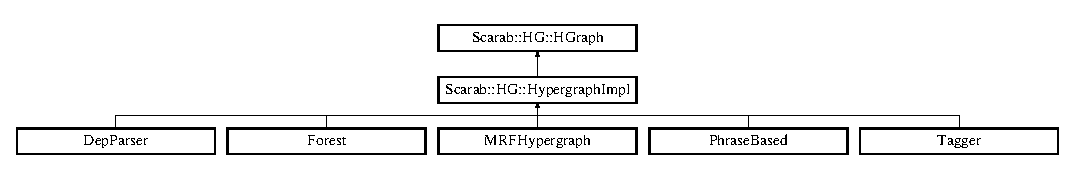
\includegraphics[height=1.85635cm]{class_scarab_1_1_h_g_1_1_hypergraph_impl}
\end{center}
\end{figure}
\subsection*{Public Member Functions}
\begin{DoxyCompactItemize}
\item 
\hypertarget{class_scarab_1_1_h_g_1_1_hypergraph_impl_a935bed9b8cf9235a1adb61d0889f6ac7}{
{\bfseries HypergraphImpl} (vector$<$ \hyperlink{class_scarab_1_1_h_g_1_1_hypernode}{Hypernode} $\ast$ $>$ nodes, vector$<$ \hyperlink{class_scarab_1_1_h_g_1_1_hyperedge}{Hyperedge} $\ast$ $>$ edges, \hyperlink{class_scarab_1_1_h_g_1_1_hypernode}{Hypernode} $\ast$root)}
\label{class_scarab_1_1_h_g_1_1_hypergraph_impl_a935bed9b8cf9235a1adb61d0889f6ac7}

\item 
const \hyperlink{class_scarab_1_1_h_g_1_1_hypernode}{Hypernode} \& \hyperlink{class_scarab_1_1_h_g_1_1_hypergraph_impl_a31172009b97d179f6b1199f191197a32}{root} () const 
\item 
\hypertarget{class_scarab_1_1_h_g_1_1_hypergraph_impl_a0adcc8783b94cbe07b092220082d00ab}{
unsigned int {\bfseries num\_\-edges} () const }
\label{class_scarab_1_1_h_g_1_1_hypergraph_impl_a0adcc8783b94cbe07b092220082d00ab}

\item 
\hypertarget{class_scarab_1_1_h_g_1_1_hypergraph_impl_ad39e917a84acb1d4caf0145ce8a903a2}{
uint {\bfseries num\_\-nodes} () const }
\label{class_scarab_1_1_h_g_1_1_hypergraph_impl_ad39e917a84acb1d4caf0145ce8a903a2}

\item 
\hypertarget{class_scarab_1_1_h_g_1_1_hypergraph_impl_a9276a6faa074eb4f3bbb2f8b8d5d4fbf}{
const \hyperlink{class_scarab_1_1_h_g_1_1_hypernode}{Hypernode} \& {\bfseries get\_\-node} (unsigned int i) const }
\label{class_scarab_1_1_h_g_1_1_hypergraph_impl_a9276a6faa074eb4f3bbb2f8b8d5d4fbf}

\item 
\hypertarget{class_scarab_1_1_h_g_1_1_hypergraph_impl_a31a148139b888b6bd10e78fe555144c7}{
const \hyperlink{class_scarab_1_1_h_g_1_1_hyperedge}{Hyperedge} \& {\bfseries get\_\-edge} (uint i) const }
\label{class_scarab_1_1_h_g_1_1_hypergraph_impl_a31a148139b888b6bd10e78fe555144c7}

\item 
\hypertarget{class_scarab_1_1_h_g_1_1_hypergraph_impl_a1f33418f90b826db9cfc0bb34e1ca9cf}{
void {\bfseries build\_\-from\_\-file} (const char $\ast$file\_\-name)}
\label{class_scarab_1_1_h_g_1_1_hypergraph_impl_a1f33418f90b826db9cfc0bb34e1ca9cf}

\item 
const vector$<$ \hyperlink{class_scarab_1_1_h_g_1_1_hypernode}{Hypernode} $\ast$ $>$ \& \hyperlink{class_scarab_1_1_h_g_1_1_hypergraph_impl_a9aef2881b489c86d4d83e996a70f8141}{nodes} () const 
\item 
const vector$<$ \hyperlink{class_scarab_1_1_h_g_1_1_hyperedge}{Hyperedge} $\ast$ $>$ \& \hyperlink{class_scarab_1_1_h_g_1_1_hypergraph_impl_a0c8373e545fe59b0cb7036b4751508e1}{edges} () const 
\item 
\hypertarget{class_scarab_1_1_h_g_1_1_hypergraph_impl_a98701d5529aaf3e5d4fa386694843f20}{
void {\bfseries prune} (const \hyperlink{struct_scarab_1_1_h_g_1_1_hypergraph_prune}{HypergraphPrune} \&prune)}
\label{class_scarab_1_1_h_g_1_1_hypergraph_impl_a98701d5529aaf3e5d4fa386694843f20}

\item 
\hypertarget{class_scarab_1_1_h_g_1_1_hypergraph_impl_af8f5ed38a355676c473e8d54b5552cc6}{
void {\bfseries write\_\-to\_\-file} (const char $\ast$file\_\-name)}
\label{class_scarab_1_1_h_g_1_1_hypergraph_impl_af8f5ed38a355676c473e8d54b5552cc6}

\end{DoxyCompactItemize}
\subsection*{Protected Member Functions}
\begin{DoxyCompactItemize}
\item 
\hypertarget{class_scarab_1_1_h_g_1_1_hypergraph_impl_af14198ba5fccb5d4118188fa42feb8ff}{
virtual \hyperlink{class_scarab_1_1_h_g_1_1_hypernode}{Hypernode} $\ast$ {\bfseries make\_\-node} (const Hypergraph\_\-Node \&node, wvector $\ast$features)}
\label{class_scarab_1_1_h_g_1_1_hypergraph_impl_af14198ba5fccb5d4118188fa42feb8ff}

\item 
\hypertarget{class_scarab_1_1_h_g_1_1_hypergraph_impl_a238a7ce3b578c8126eccbc7803570638}{
virtual void {\bfseries make\_\-edge} (const Hypergraph\_\-Edge \&edge, const \hyperlink{class_scarab_1_1_h_g_1_1_hyperedge}{Hyperedge} $\ast$our\_\-edge)}
\label{class_scarab_1_1_h_g_1_1_hypergraph_impl_a238a7ce3b578c8126eccbc7803570638}

\item 
\hypertarget{class_scarab_1_1_h_g_1_1_hypergraph_impl_a30349aca0e3b8f8dc72ed74d78e8c5b8}{
virtual void {\bfseries convert\_\-edge} (const \hyperlink{class_scarab_1_1_h_g_1_1_hyperedge}{Hyperedge} $\ast$our\_\-edge, Hypergraph\_\-Edge $\ast$edge)}
\label{class_scarab_1_1_h_g_1_1_hypergraph_impl_a30349aca0e3b8f8dc72ed74d78e8c5b8}

\item 
\hypertarget{class_scarab_1_1_h_g_1_1_hypergraph_impl_a93e9e250fa457a2171bf07241b7829eb}{
virtual void {\bfseries convert\_\-node} (const \hyperlink{class_scarab_1_1_h_g_1_1_hypernode}{Hypernode} $\ast$our\_\-node, Hypergraph\_\-Node $\ast$node)}
\label{class_scarab_1_1_h_g_1_1_hypergraph_impl_a93e9e250fa457a2171bf07241b7829eb}

\item 
\hypertarget{class_scarab_1_1_h_g_1_1_hypergraph_impl_ae91de73e633e450b01664e3ec964019c}{
virtual void {\bfseries set\_\-up} (const Hypergraph \&hgraph)}
\label{class_scarab_1_1_h_g_1_1_hypergraph_impl_ae91de73e633e450b01664e3ec964019c}

\end{DoxyCompactItemize}
\subsection*{Protected Attributes}
\begin{DoxyCompactItemize}
\item 
\hypertarget{class_scarab_1_1_h_g_1_1_hypergraph_impl_aa7192cf8f168e5bfed67a8faf85c8cb4}{
::Hypergraph $\ast$ {\bfseries hgraph}}
\label{class_scarab_1_1_h_g_1_1_hypergraph_impl_aa7192cf8f168e5bfed67a8faf85c8cb4}

\item 
\hypertarget{class_scarab_1_1_h_g_1_1_hypergraph_impl_a7035fdae4c04d0752aaaf1e7eba7600e}{
\hyperlink{class_scarab_1_1_h_g_1_1_hypernode}{Hypernode} $\ast$ {\bfseries \_\-root}}
\label{class_scarab_1_1_h_g_1_1_hypergraph_impl_a7035fdae4c04d0752aaaf1e7eba7600e}

\item 
\hypertarget{class_scarab_1_1_h_g_1_1_hypergraph_impl_a4cc57d9255e2f09714c5913d67cd0554}{
vector$<$ \hyperlink{class_scarab_1_1_h_g_1_1_hypernode}{Hypernode} $\ast$ $>$ {\bfseries \_\-nodes}}
\label{class_scarab_1_1_h_g_1_1_hypergraph_impl_a4cc57d9255e2f09714c5913d67cd0554}

\item 
\hypertarget{class_scarab_1_1_h_g_1_1_hypergraph_impl_a56fb710140f3359646b1a17cb0417d74}{
vector$<$ \hyperlink{class_scarab_1_1_h_g_1_1_hyperedge}{Hyperedge} $\ast$ $>$ {\bfseries \_\-edges}}
\label{class_scarab_1_1_h_g_1_1_hypergraph_impl_a56fb710140f3359646b1a17cb0417d74}

\end{DoxyCompactItemize}


\subsection{Member Function Documentation}
\hypertarget{class_scarab_1_1_h_g_1_1_hypergraph_impl_a0c8373e545fe59b0cb7036b4751508e1}{
\index{Scarab::HG::HypergraphImpl@{Scarab::HG::HypergraphImpl}!edges@{edges}}
\index{edges@{edges}!Scarab::HG::HypergraphImpl@{Scarab::HG::HypergraphImpl}}
\subsubsection[{edges}]{\setlength{\rightskip}{0pt plus 5cm}const vector$<${\bf Hyperedge}$\ast$$>$\& Scarab::HG::HypergraphImpl::edges () const\hspace{0.3cm}{\ttfamily  \mbox{[}inline, virtual\mbox{]}}}}
\label{class_scarab_1_1_h_g_1_1_hypergraph_impl_a0c8373e545fe59b0cb7036b4751508e1}
Get all hyperedges in the hypergraph. (Assume unordered) WARNING: Treat this as a const iterator. \begin{DoxyReturn}{Returns}
Const iterator to edges in hypergraph . 
\end{DoxyReturn}


Implements \hyperlink{class_scarab_1_1_h_g_1_1_h_graph_a57328729f90cc4152ca79ff15ecdd4bb}{Scarab::HG::HGraph}.

\hypertarget{class_scarab_1_1_h_g_1_1_hypergraph_impl_a9aef2881b489c86d4d83e996a70f8141}{
\index{Scarab::HG::HypergraphImpl@{Scarab::HG::HypergraphImpl}!nodes@{nodes}}
\index{nodes@{nodes}!Scarab::HG::HypergraphImpl@{Scarab::HG::HypergraphImpl}}
\subsubsection[{nodes}]{\setlength{\rightskip}{0pt plus 5cm}const vector$<${\bf Hypernode}$\ast$$>$\& Scarab::HG::HypergraphImpl::nodes () const\hspace{0.3cm}{\ttfamily  \mbox{[}inline, virtual\mbox{]}}}}
\label{class_scarab_1_1_h_g_1_1_hypergraph_impl_a9aef2881b489c86d4d83e996a70f8141}
Get all hypernodes in the hypergraph. (Assume unordered) WARNING: Treat this as a const iterator. \begin{DoxyReturn}{Returns}
Const iterator to hypernodes in hypergraph . 
\end{DoxyReturn}


Implements \hyperlink{class_scarab_1_1_h_g_1_1_h_graph_a74d893fba015520774f71f02a46bb6ca}{Scarab::HG::HGraph}.

\hypertarget{class_scarab_1_1_h_g_1_1_hypergraph_impl_a31172009b97d179f6b1199f191197a32}{
\index{Scarab::HG::HypergraphImpl@{Scarab::HG::HypergraphImpl}!root@{root}}
\index{root@{root}!Scarab::HG::HypergraphImpl@{Scarab::HG::HypergraphImpl}}
\subsubsection[{root}]{\setlength{\rightskip}{0pt plus 5cm}const {\bf Hypernode}\& Scarab::HG::HypergraphImpl::root () const\hspace{0.3cm}{\ttfamily  \mbox{[}inline, virtual\mbox{]}}}}
\label{class_scarab_1_1_h_g_1_1_hypergraph_impl_a31172009b97d179f6b1199f191197a32}
Get the root of the hypergraph

\begin{DoxyReturn}{Returns}
\hyperlink{class_scarab_1_1_h_g_1_1_hypernode}{Hypernode} at root 
\end{DoxyReturn}


Implements \hyperlink{class_scarab_1_1_h_g_1_1_h_graph_a5ede392b158e41dd7e95ded1c4b0b5d6}{Scarab::HG::HGraph}.



The documentation for this class was generated from the following files:\begin{DoxyCompactItemize}
\item 
hypergraph/HypergraphImpl.h\item 
hypergraph/HypergraphImpl.cpp\end{DoxyCompactItemize}

\hypertarget{struct_scarab_1_1_h_g_1_1_hypergraph_l_p}{
\section{Scarab::HG::HypergraphLP Struct Reference}
\label{struct_scarab_1_1_h_g_1_1_hypergraph_l_p}\index{Scarab::HG::HypergraphLP@{Scarab::HG::HypergraphLP}}
}
\subsection*{Public Member Functions}
\begin{DoxyCompactItemize}
\item 
\hypertarget{struct_scarab_1_1_h_g_1_1_hypergraph_l_p_a332edf79e5fc5b617ec6e948a73cc4a4}{
{\bfseries HypergraphLP} (const \hyperlink{class_scarab_1_1_h_g_1_1_h_graph}{HGraph} \&h)}
\label{struct_scarab_1_1_h_g_1_1_hypergraph_l_p_a332edf79e5fc5b617ec6e948a73cc4a4}

\end{DoxyCompactItemize}
\subsection*{Public Attributes}
\begin{DoxyCompactItemize}
\item 
\hypertarget{struct_scarab_1_1_h_g_1_1_hypergraph_l_p_ae9c9c441b112e98e412e8129e91a28ce}{
\hyperlink{class_cache}{Cache}$<$ \hyperlink{class_scarab_1_1_h_g_1_1_hypernode}{Hypernode}, GRBVar $>$ {\bfseries node\_\-vars}}
\label{struct_scarab_1_1_h_g_1_1_hypergraph_l_p_ae9c9c441b112e98e412e8129e91a28ce}

\item 
\hypertarget{struct_scarab_1_1_h_g_1_1_hypergraph_l_p_a8e71b062f3d6691eef27bb85c718604f}{
\hyperlink{class_cache}{Cache}$<$ \hyperlink{class_scarab_1_1_h_g_1_1_hyperedge}{Hyperedge}, GRBVar $>$ {\bfseries edge\_\-vars}}
\label{struct_scarab_1_1_h_g_1_1_hypergraph_l_p_a8e71b062f3d6691eef27bb85c718604f}

\item 
\hypertarget{struct_scarab_1_1_h_g_1_1_hypergraph_l_p_a52fa717afa9c902f7d8ef3adf18c5204}{
const \hyperlink{class_scarab_1_1_h_g_1_1_h_graph}{HGraph} \& {\bfseries \_\-h}}
\label{struct_scarab_1_1_h_g_1_1_hypergraph_l_p_a52fa717afa9c902f7d8ef3adf18c5204}

\end{DoxyCompactItemize}


The documentation for this struct was generated from the following file:\begin{DoxyCompactItemize}
\item 
lp/HypergraphLP.h\end{DoxyCompactItemize}

\hypertarget{class_scarab_1_1_h_g_1_1_hypergraph_l_p_builder}{
\section{Scarab::HG::HypergraphLPBuilder Class Reference}
\label{class_scarab_1_1_h_g_1_1_hypergraph_l_p_builder}\index{Scarab::HG::HypergraphLPBuilder@{Scarab::HG::HypergraphLPBuilder}}
}
\subsection*{Static Public Member Functions}
\begin{DoxyCompactItemize}
\item 
\hypertarget{class_scarab_1_1_h_g_1_1_hypergraph_l_p_builder_a7653a6f997f1505c0d6668618b28d6d8}{
static void {\bfseries show\_\-hypergraph} (const \hyperlink{struct_scarab_1_1_h_g_1_1_hypergraph_l_p}{HypergraphLP} \&h\_\-lp)}
\label{class_scarab_1_1_h_g_1_1_hypergraph_l_p_builder_a7653a6f997f1505c0d6668618b28d6d8}

\item 
\hypertarget{class_scarab_1_1_h_g_1_1_hypergraph_l_p_builder_a3a711a79152e0f5d4cc9157737673b95}{
static \hyperlink{struct_scarab_1_1_h_g_1_1_hypergraph_l_p}{HypergraphLP} $\ast$ {\bfseries add\_\-hypergraph} (const \hyperlink{class_scarab_1_1_h_g_1_1_h_graph}{HGraph} \&h, const \hyperlink{class_cache}{Cache}$<$ \hyperlink{class_scarab_1_1_h_g_1_1_hyperedge}{Hyperedge}, double $>$ \&\_\-weights, string prefix, GRBModel \&model, int var\_\-type)}
\label{class_scarab_1_1_h_g_1_1_hypergraph_l_p_builder_a3a711a79152e0f5d4cc9157737673b95}

\end{DoxyCompactItemize}


The documentation for this class was generated from the following file:\begin{DoxyCompactItemize}
\item 
lp/HypergraphLP.h\end{DoxyCompactItemize}

\hypertarget{struct_scarab_1_1_h_g_1_1_hypergraph_prune}{
\section{Scarab::HG::HypergraphPrune Struct Reference}
\label{struct_scarab_1_1_h_g_1_1_hypergraph_prune}\index{Scarab::HG::HypergraphPrune@{Scarab::HG::HypergraphPrune}}
}
\subsection*{Public Member Functions}
\begin{DoxyCompactItemize}
\item 
\hypertarget{struct_scarab_1_1_h_g_1_1_hypergraph_prune_adc29528f39ad9ced03be8b48341c3e84}{
{\bfseries HypergraphPrune} (const \hyperlink{class_scarab_1_1_h_g_1_1_h_graph}{HGraph} \&hgraph\_\-)}
\label{struct_scarab_1_1_h_g_1_1_hypergraph_prune_adc29528f39ad9ced03be8b48341c3e84}

\end{DoxyCompactItemize}
\subsection*{Public Attributes}
\begin{DoxyCompactItemize}
\item 
\hypertarget{struct_scarab_1_1_h_g_1_1_hypergraph_prune_a1ff0fd7b723f888db33ae542d186d0b4}{
set$<$ int $>$ {\bfseries nodes}}
\label{struct_scarab_1_1_h_g_1_1_hypergraph_prune_a1ff0fd7b723f888db33ae542d186d0b4}

\item 
\hypertarget{struct_scarab_1_1_h_g_1_1_hypergraph_prune_adff9a55407cd2cff9199d440ef513029}{
set$<$ int $>$ {\bfseries edges}}
\label{struct_scarab_1_1_h_g_1_1_hypergraph_prune_adff9a55407cd2cff9199d440ef513029}

\item 
\hypertarget{struct_scarab_1_1_h_g_1_1_hypergraph_prune_a55f12db438013ace2d307efb284bcb7b}{
const \hyperlink{class_scarab_1_1_h_g_1_1_h_graph}{HGraph} \& {\bfseries hgraph}}
\label{struct_scarab_1_1_h_g_1_1_hypergraph_prune_a55f12db438013ace2d307efb284bcb7b}

\end{DoxyCompactItemize}


The documentation for this struct was generated from the following file:\begin{DoxyCompactItemize}
\item 
hypergraph/Hypergraph.h\end{DoxyCompactItemize}

\hypertarget{class_hypergraph_tools}{
\section{HypergraphTools Class Reference}
\label{class_hypergraph_tools}\index{HypergraphTools@{HypergraphTools}}
}
\subsection*{Public Member Functions}
\begin{DoxyCompactItemize}
\item 
\hypertarget{class_hypergraph_tools_a188643770705ed9482616956e22ebfd4}{
void {\bfseries viterbi} (HGraph g)}
\label{class_hypergraph_tools_a188643770705ed9482616956e22ebfd4}

\end{DoxyCompactItemize}


The documentation for this class was generated from the following file:\begin{DoxyCompactItemize}
\item 
hypergraph/HypergraphTools.h\end{DoxyCompactItemize}

\hypertarget{class_scarab_1_1_h_g_1_1_hypernode}{
\section{Scarab::HG::Hypernode Class Reference}
\label{class_scarab_1_1_h_g_1_1_hypernode}\index{Scarab::HG::Hypernode@{Scarab::HG::Hypernode}}
}


{\ttfamily \#include $<$Hypergraph.h$>$}

Inheritance diagram for Scarab::HG::Hypernode:\begin{figure}[H]
\begin{center}
\leavevmode
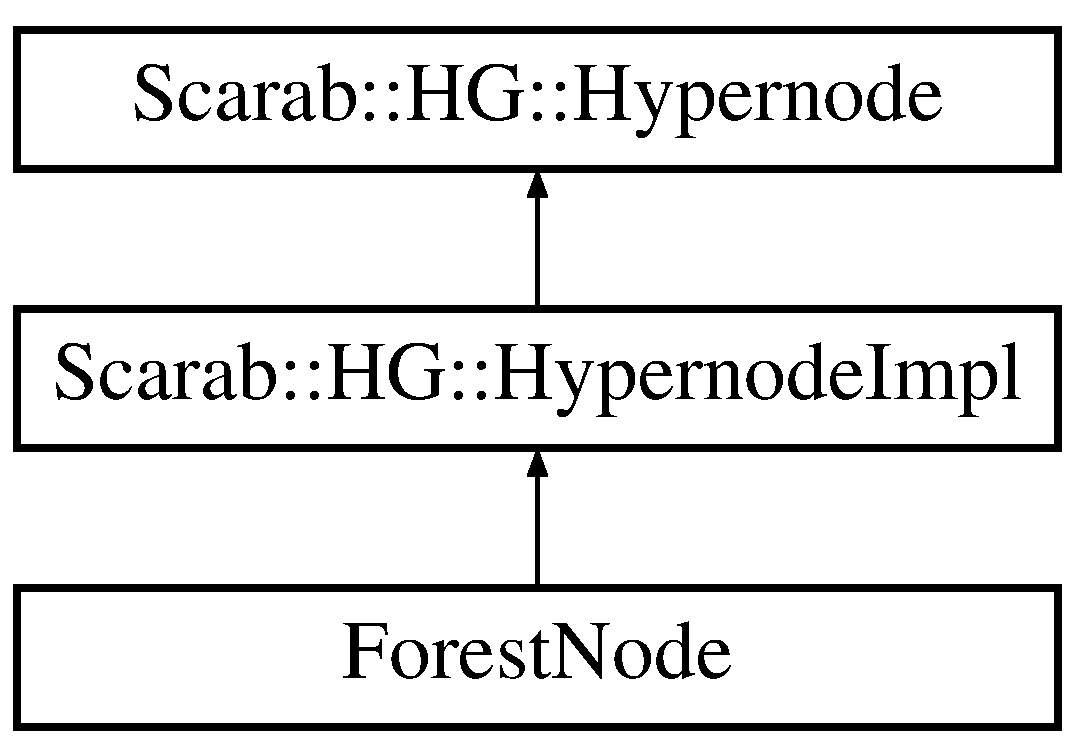
\includegraphics[height=3cm]{class_scarab_1_1_h_g_1_1_hypernode}
\end{center}
\end{figure}
\subsection*{Public Member Functions}
\begin{DoxyCompactItemize}
\item 
virtual \hyperlink{class_scarab_1_1_h_g_1_1_hypernode_a0657cc96f62d29da3ae4b5b9bcab1ce6}{$\sim$Hypernode} ()
\item 
virtual unsigned int \hyperlink{class_scarab_1_1_h_g_1_1_hypernode_a0aeaee6c2ca2a011fcd086f803aaa4d0}{id} () const =0
\item 
virtual unsigned int \hyperlink{class_scarab_1_1_h_g_1_1_hypernode_add2f4d556be223b906bfbab9f1b60870}{num\_\-edges} () const =0
\item 
virtual unsigned int \hyperlink{class_scarab_1_1_h_g_1_1_hypernode_a4b1a4ffaa8a8b0295763673e6d86d693}{num\_\-in\_\-edges} () const =0
\item 
virtual const \hyperlink{class_scarab_1_1_h_g_1_1_hyperedge}{Hyperedge} \& \hyperlink{class_scarab_1_1_h_g_1_1_hypernode_a3bface6832eb54a00d90e4fe8d1999f7}{edge} (unsigned int i) const =0
\item 
virtual const \hyperlink{class_scarab_1_1_h_g_1_1_hyperedge}{Hyperedge} \& \hyperlink{class_scarab_1_1_h_g_1_1_hypernode_a533d3e0bc2269ec07edbda32305daf70}{in\_\-edge} (unsigned int i) const =0
\item 
virtual bool \hyperlink{class_scarab_1_1_h_g_1_1_hypernode_ae3e1107309a8817d1015bd70a90c1c49}{is\_\-terminal} () const =0
\item 
virtual const vector$<$ \hyperlink{class_scarab_1_1_h_g_1_1_hyperedge}{Hyperedge} $\ast$ $>$ \& \hyperlink{class_scarab_1_1_h_g_1_1_hypernode_a3306572ded5b5061c1916bcf268be94e}{edges} () const =0
\item 
virtual const vector$<$ \hyperlink{class_scarab_1_1_h_g_1_1_hyperedge}{Hyperedge} $\ast$ $>$ \& \hyperlink{class_scarab_1_1_h_g_1_1_hypernode_aad118748408663b8242dc52d45bbd49d}{in\_\-edges} () const =0
\end{DoxyCompactItemize}


\subsection{Detailed Description}
\hyperlink{class_scarab_1_1_h_g_1_1_hypernode}{Hypernode} -\/ Constant representation of a hypernode in a hypergraph. Accessors for edges above and below. 

\subsection{Constructor \& Destructor Documentation}
\hypertarget{class_scarab_1_1_h_g_1_1_hypernode_a0657cc96f62d29da3ae4b5b9bcab1ce6}{
\index{Scarab::HG::Hypernode@{Scarab::HG::Hypernode}!$\sim$Hypernode@{$\sim$Hypernode}}
\index{$\sim$Hypernode@{$\sim$Hypernode}!Scarab::HG::Hypernode@{Scarab::HG::Hypernode}}
\subsubsection[{$\sim$Hypernode}]{\setlength{\rightskip}{0pt plus 5cm}virtual Scarab::HG::Hypernode::$\sim$Hypernode ()\hspace{0.3cm}{\ttfamily  \mbox{[}inline, virtual\mbox{]}}}}
\label{class_scarab_1_1_h_g_1_1_hypernode_a0657cc96f62d29da3ae4b5b9bcab1ce6}
WARNING: Private except to Hypergraph 

\subsection{Member Function Documentation}
\hypertarget{class_scarab_1_1_h_g_1_1_hypernode_a3bface6832eb54a00d90e4fe8d1999f7}{
\index{Scarab::HG::Hypernode@{Scarab::HG::Hypernode}!edge@{edge}}
\index{edge@{edge}!Scarab::HG::Hypernode@{Scarab::HG::Hypernode}}
\subsubsection[{edge}]{\setlength{\rightskip}{0pt plus 5cm}virtual const {\bf Hyperedge}\& Scarab::HG::Hypernode::edge (unsigned int {\em i}) const\hspace{0.3cm}{\ttfamily  \mbox{[}pure virtual\mbox{]}}}}
\label{class_scarab_1_1_h_g_1_1_hypernode_a3bface6832eb54a00d90e4fe8d1999f7}
Get the hyperedge this node as head \begin{Desc}
\item[\hyperlink{deprecated__deprecated000009}{Deprecated}]\end{Desc}

\begin{DoxyParams}{Parameters}
\item[{\em i}]Local local id of edge\end{DoxyParams}
\begin{DoxyReturn}{Returns}
The hyperedge 
\end{DoxyReturn}


Implemented in \hyperlink{class_scarab_1_1_h_g_1_1_hypernode_impl_a328189f28a4185d435035686a27592c2}{Scarab::HG::HypernodeImpl}.

\hypertarget{class_scarab_1_1_h_g_1_1_hypernode_a3306572ded5b5061c1916bcf268be94e}{
\index{Scarab::HG::Hypernode@{Scarab::HG::Hypernode}!edges@{edges}}
\index{edges@{edges}!Scarab::HG::Hypernode@{Scarab::HG::Hypernode}}
\subsubsection[{edges}]{\setlength{\rightskip}{0pt plus 5cm}virtual const vector$<${\bf Hyperedge}$\ast$$>$\& Scarab::HG::Hypernode::edges () const\hspace{0.3cm}{\ttfamily  \mbox{[}pure virtual\mbox{]}}}}
\label{class_scarab_1_1_h_g_1_1_hypernode_a3306572ded5b5061c1916bcf268be94e}
Get all hyperedges with this hypernode as head. WARNING: Treat this as a const iterator. \begin{DoxyReturn}{Returns}
Const iterator to edges. 
\end{DoxyReturn}


Implemented in \hyperlink{class_scarab_1_1_h_g_1_1_hypernode_impl_ada979dcddc1bf0abf0fc2530d1ea8761}{Scarab::HG::HypernodeImpl}.

\hypertarget{class_scarab_1_1_h_g_1_1_hypernode_a0aeaee6c2ca2a011fcd086f803aaa4d0}{
\index{Scarab::HG::Hypernode@{Scarab::HG::Hypernode}!id@{id}}
\index{id@{id}!Scarab::HG::Hypernode@{Scarab::HG::Hypernode}}
\subsubsection[{id}]{\setlength{\rightskip}{0pt plus 5cm}virtual unsigned int Scarab::HG::Hypernode::id () const\hspace{0.3cm}{\ttfamily  \mbox{[}pure virtual\mbox{]}}}}
\label{class_scarab_1_1_h_g_1_1_hypernode_a0aeaee6c2ca2a011fcd086f803aaa4d0}
The unique identifier of the \hyperlink{class_scarab_1_1_h_g_1_1_hypernode}{Hypernode} \begin{Desc}
\item[\hyperlink{deprecated__deprecated000006}{Deprecated}]\end{Desc}
\begin{DoxyReturn}{Returns}
The number 
\end{DoxyReturn}


Implemented in \hyperlink{class_scarab_1_1_h_g_1_1_hypernode_impl_a2579ef1e67ad8f51d23838c130440d21}{Scarab::HG::HypernodeImpl}.

\hypertarget{class_scarab_1_1_h_g_1_1_hypernode_a533d3e0bc2269ec07edbda32305daf70}{
\index{Scarab::HG::Hypernode@{Scarab::HG::Hypernode}!in\_\-edge@{in\_\-edge}}
\index{in\_\-edge@{in\_\-edge}!Scarab::HG::Hypernode@{Scarab::HG::Hypernode}}
\subsubsection[{in\_\-edge}]{\setlength{\rightskip}{0pt plus 5cm}virtual const {\bf Hyperedge}\& Scarab::HG::Hypernode::in\_\-edge (unsigned int {\em i}) const\hspace{0.3cm}{\ttfamily  \mbox{[}pure virtual\mbox{]}}}}
\label{class_scarab_1_1_h_g_1_1_hypernode_a533d3e0bc2269ec07edbda32305daf70}
Get the hyperedge this node as tail \begin{Desc}
\item[\hyperlink{deprecated__deprecated000010}{Deprecated}]\end{Desc}

\begin{DoxyParams}{Parameters}
\item[{\em i}]Local local id of edge\end{DoxyParams}
\begin{DoxyReturn}{Returns}
The hyperedge 
\end{DoxyReturn}


Implemented in \hyperlink{class_scarab_1_1_h_g_1_1_hypernode_impl_a26ff9db30c03c7b74181e9f901aa71d4}{Scarab::HG::HypernodeImpl}.

\hypertarget{class_scarab_1_1_h_g_1_1_hypernode_aad118748408663b8242dc52d45bbd49d}{
\index{Scarab::HG::Hypernode@{Scarab::HG::Hypernode}!in\_\-edges@{in\_\-edges}}
\index{in\_\-edges@{in\_\-edges}!Scarab::HG::Hypernode@{Scarab::HG::Hypernode}}
\subsubsection[{in\_\-edges}]{\setlength{\rightskip}{0pt plus 5cm}virtual const vector$<${\bf Hyperedge}$\ast$$>$\& Scarab::HG::Hypernode::in\_\-edges () const\hspace{0.3cm}{\ttfamily  \mbox{[}pure virtual\mbox{]}}}}
\label{class_scarab_1_1_h_g_1_1_hypernode_aad118748408663b8242dc52d45bbd49d}
Get all hyperedges with this hypernode as a tail. WARNING: Treat this as a const iterator. \begin{DoxyReturn}{Returns}
Const iterator to edges. 
\end{DoxyReturn}


Implemented in \hyperlink{class_scarab_1_1_h_g_1_1_hypernode_impl_a77fe0de2e3927be6145cb8fc018088c9}{Scarab::HG::HypernodeImpl}.

\hypertarget{class_scarab_1_1_h_g_1_1_hypernode_ae3e1107309a8817d1015bd70a90c1c49}{
\index{Scarab::HG::Hypernode@{Scarab::HG::Hypernode}!is\_\-terminal@{is\_\-terminal}}
\index{is\_\-terminal@{is\_\-terminal}!Scarab::HG::Hypernode@{Scarab::HG::Hypernode}}
\subsubsection[{is\_\-terminal}]{\setlength{\rightskip}{0pt plus 5cm}virtual bool Scarab::HG::Hypernode::is\_\-terminal () const\hspace{0.3cm}{\ttfamily  \mbox{[}pure virtual\mbox{]}}}}
\label{class_scarab_1_1_h_g_1_1_hypernode_ae3e1107309a8817d1015bd70a90c1c49}
Is this node a terminal nodes. (no children)

\begin{DoxyReturn}{Returns}
True if terminal (assert \hyperlink{class_scarab_1_1_h_g_1_1_hypernode_ae3e1107309a8817d1015bd70a90c1c49}{is\_\-terminal()} == (\hyperlink{class_scarab_1_1_h_g_1_1_hypernode_add2f4d556be223b906bfbab9f1b60870}{num\_\-edges()} == 0)) 
\end{DoxyReturn}


Implemented in \hyperlink{class_scarab_1_1_h_g_1_1_hypernode_impl_a2bb4b33ff207c3c1babe135b9af6323e}{Scarab::HG::HypernodeImpl}.

\hypertarget{class_scarab_1_1_h_g_1_1_hypernode_add2f4d556be223b906bfbab9f1b60870}{
\index{Scarab::HG::Hypernode@{Scarab::HG::Hypernode}!num\_\-edges@{num\_\-edges}}
\index{num\_\-edges@{num\_\-edges}!Scarab::HG::Hypernode@{Scarab::HG::Hypernode}}
\subsubsection[{num\_\-edges}]{\setlength{\rightskip}{0pt plus 5cm}virtual unsigned int Scarab::HG::Hypernode::num\_\-edges () const\hspace{0.3cm}{\ttfamily  \mbox{[}pure virtual\mbox{]}}}}
\label{class_scarab_1_1_h_g_1_1_hypernode_add2f4d556be223b906bfbab9f1b60870}
Get the number of hyperedges that have this node as head \begin{Desc}
\item[\hyperlink{deprecated__deprecated000007}{Deprecated}]\end{Desc}
\begin{DoxyReturn}{Returns}
The number 
\end{DoxyReturn}


Implemented in \hyperlink{class_scarab_1_1_h_g_1_1_hypernode_impl_a7fed4809706319cc916ed4c04a641436}{Scarab::HG::HypernodeImpl}.

\hypertarget{class_scarab_1_1_h_g_1_1_hypernode_a4b1a4ffaa8a8b0295763673e6d86d693}{
\index{Scarab::HG::Hypernode@{Scarab::HG::Hypernode}!num\_\-in\_\-edges@{num\_\-in\_\-edges}}
\index{num\_\-in\_\-edges@{num\_\-in\_\-edges}!Scarab::HG::Hypernode@{Scarab::HG::Hypernode}}
\subsubsection[{num\_\-in\_\-edges}]{\setlength{\rightskip}{0pt plus 5cm}virtual unsigned int Scarab::HG::Hypernode::num\_\-in\_\-edges () const\hspace{0.3cm}{\ttfamily  \mbox{[}pure virtual\mbox{]}}}}
\label{class_scarab_1_1_h_g_1_1_hypernode_a4b1a4ffaa8a8b0295763673e6d86d693}
Get the number of hyperedges that have this node as tail \begin{Desc}
\item[\hyperlink{deprecated__deprecated000008}{Deprecated}]\end{Desc}
\begin{DoxyReturn}{Returns}
The number 
\end{DoxyReturn}


Implemented in \hyperlink{class_scarab_1_1_h_g_1_1_hypernode_impl_a9a13a37fcece16603ec4bf3f364e6fcc}{Scarab::HG::HypernodeImpl}.



The documentation for this class was generated from the following file:\begin{DoxyCompactItemize}
\item 
hypergraph/Hypergraph.h\end{DoxyCompactItemize}

\hypertarget{class_scarab_1_1_h_g_1_1_hypernode_impl}{
\section{Scarab::HG::HypernodeImpl Class Reference}
\label{class_scarab_1_1_h_g_1_1_hypernode_impl}\index{Scarab::HG::HypernodeImpl@{Scarab::HG::HypernodeImpl}}
}
Inheritance diagram for Scarab::HG::HypernodeImpl:\begin{figure}[H]
\begin{center}
\leavevmode
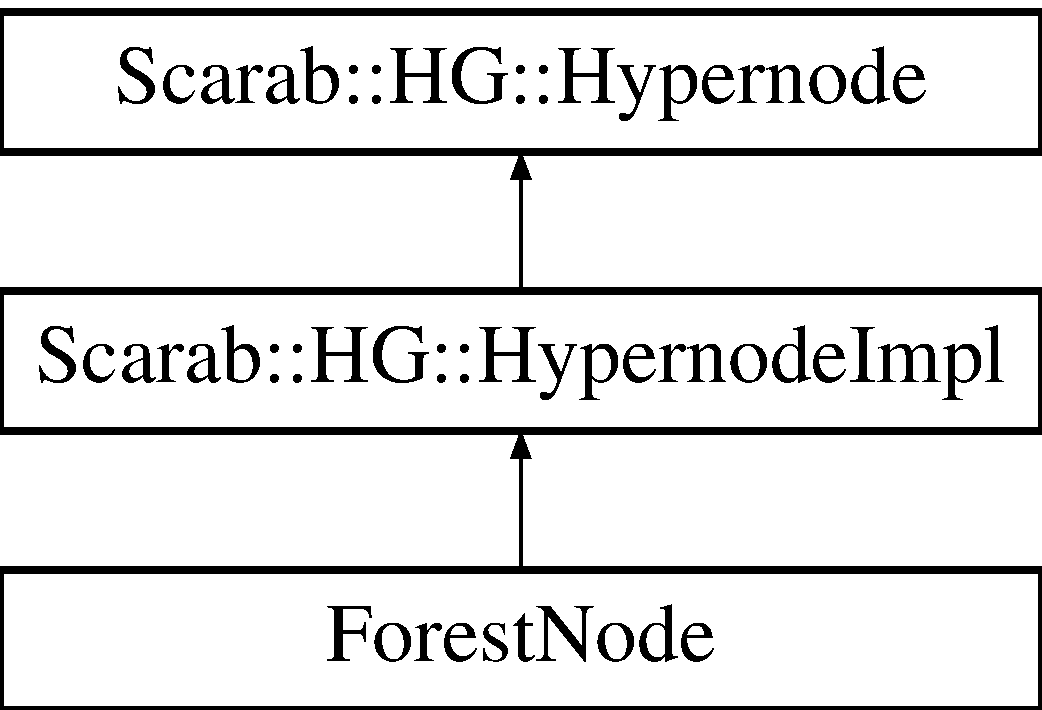
\includegraphics[height=3cm]{class_scarab_1_1_h_g_1_1_hypernode_impl}
\end{center}
\end{figure}
\subsection*{Public Member Functions}
\begin{DoxyCompactItemize}
\item 
\hypertarget{class_scarab_1_1_h_g_1_1_hypernode_impl_a574c6f1386fb27894075977ef1ca56d6}{
{\bfseries HypernodeImpl} (const string \&label, int id, wvector $\ast$features)}
\label{class_scarab_1_1_h_g_1_1_hypernode_impl_a574c6f1386fb27894075977ef1ca56d6}

\item 
\hypertarget{class_scarab_1_1_h_g_1_1_hypernode_impl_a0899a4e97f535c2f005d7c5ab5364681}{
void {\bfseries add\_\-edge} (\hyperlink{class_scarab_1_1_h_g_1_1_hyperedge}{Hyperedge} $\ast$edge)}
\label{class_scarab_1_1_h_g_1_1_hypernode_impl_a0899a4e97f535c2f005d7c5ab5364681}

\item 
\hypertarget{class_scarab_1_1_h_g_1_1_hypernode_impl_ab05500702d5fa1c896efe941f9c54bf3}{
void {\bfseries add\_\-in\_\-edge} (\hyperlink{class_scarab_1_1_h_g_1_1_hyperedge}{Hyperedge} $\ast$edge)}
\label{class_scarab_1_1_h_g_1_1_hypernode_impl_ab05500702d5fa1c896efe941f9c54bf3}

\item 
bool \hyperlink{class_scarab_1_1_h_g_1_1_hypernode_impl_a2bb4b33ff207c3c1babe135b9af6323e}{is\_\-terminal} () const 
\item 
\hypertarget{class_scarab_1_1_h_g_1_1_hypernode_impl_a6675d677bd7e794ae9a8bf72645b828a}{
void {\bfseries prune\_\-edges} (const set$<$ int $>$ \&keep\_\-edges)}
\label{class_scarab_1_1_h_g_1_1_hypernode_impl_a6675d677bd7e794ae9a8bf72645b828a}

\item 
const \hyperlink{class_scarab_1_1_h_g_1_1_hyperedge}{Hyperedge} \& \hyperlink{class_scarab_1_1_h_g_1_1_hypernode_impl_a328189f28a4185d435035686a27592c2}{edge} (uint i) const 
\item 
unsigned int \hyperlink{class_scarab_1_1_h_g_1_1_hypernode_impl_a7fed4809706319cc916ed4c04a641436}{num\_\-edges} () const 
\item 
unsigned int \hyperlink{class_scarab_1_1_h_g_1_1_hypernode_impl_a9a13a37fcece16603ec4bf3f364e6fcc}{num\_\-in\_\-edges} () const 
\item 
const \hyperlink{class_scarab_1_1_h_g_1_1_hyperedge}{Hyperedge} \& \hyperlink{class_scarab_1_1_h_g_1_1_hypernode_impl_a26ff9db30c03c7b74181e9f901aa71d4}{in\_\-edge} (uint i) const 
\item 
uint \hyperlink{class_scarab_1_1_h_g_1_1_hypernode_impl_a2579ef1e67ad8f51d23838c130440d21}{id} () const 
\item 
const vector$<$ \hyperlink{class_scarab_1_1_h_g_1_1_hyperedge}{Hyperedge} $\ast$ $>$ \& \hyperlink{class_scarab_1_1_h_g_1_1_hypernode_impl_ada979dcddc1bf0abf0fc2530d1ea8761}{edges} () const 
\item 
const vector$<$ \hyperlink{class_scarab_1_1_h_g_1_1_hyperedge}{Hyperedge} $\ast$ $>$ \& \hyperlink{class_scarab_1_1_h_g_1_1_hypernode_impl_a77fe0de2e3927be6145cb8fc018088c9}{in\_\-edges} () const 
\item 
\hypertarget{class_scarab_1_1_h_g_1_1_hypernode_impl_a9b0df10dfd6c20c094a928f1ced76f90}{
void {\bfseries reid} (int new\_\-id)}
\label{class_scarab_1_1_h_g_1_1_hypernode_impl_a9b0df10dfd6c20c094a928f1ced76f90}

\end{DoxyCompactItemize}
\subsection*{Public Attributes}
\begin{DoxyCompactItemize}
\item 
\hypertarget{class_scarab_1_1_h_g_1_1_hypernode_impl_aaa189784dcf714f3c1ca54ea8cd0dc83}{
vector$<$ \hyperlink{class_scarab_1_1_h_g_1_1_hyperedge}{Hyperedge} $\ast$ $>$ {\bfseries \_\-edges}}
\label{class_scarab_1_1_h_g_1_1_hypernode_impl_aaa189784dcf714f3c1ca54ea8cd0dc83}

\item 
\hypertarget{class_scarab_1_1_h_g_1_1_hypernode_impl_aefb3b14843d6fb8ed2284ae0d6a53dbd}{
const string \& {\bfseries \_\-label}}
\label{class_scarab_1_1_h_g_1_1_hypernode_impl_aefb3b14843d6fb8ed2284ae0d6a53dbd}

\end{DoxyCompactItemize}


\subsection{Member Function Documentation}
\hypertarget{class_scarab_1_1_h_g_1_1_hypernode_impl_a328189f28a4185d435035686a27592c2}{
\index{Scarab::HG::HypernodeImpl@{Scarab::HG::HypernodeImpl}!edge@{edge}}
\index{edge@{edge}!Scarab::HG::HypernodeImpl@{Scarab::HG::HypernodeImpl}}
\subsubsection[{edge}]{\setlength{\rightskip}{0pt plus 5cm}const {\bf Hyperedge}\& Scarab::HG::HypernodeImpl::edge (uint {\em i}) const\hspace{0.3cm}{\ttfamily  \mbox{[}inline, virtual\mbox{]}}}}
\label{class_scarab_1_1_h_g_1_1_hypernode_impl_a328189f28a4185d435035686a27592c2}
Get the hyperedge this node as head \begin{Desc}
\item[\hyperlink{deprecated__deprecated000009}{Deprecated}]\end{Desc}

\begin{DoxyParams}{Parameters}
\item[{\em i}]Local local id of edge\end{DoxyParams}
\begin{DoxyReturn}{Returns}
The hyperedge 
\end{DoxyReturn}


Implements \hyperlink{class_scarab_1_1_h_g_1_1_hypernode_a3bface6832eb54a00d90e4fe8d1999f7}{Scarab::HG::Hypernode}.

\hypertarget{class_scarab_1_1_h_g_1_1_hypernode_impl_ada979dcddc1bf0abf0fc2530d1ea8761}{
\index{Scarab::HG::HypernodeImpl@{Scarab::HG::HypernodeImpl}!edges@{edges}}
\index{edges@{edges}!Scarab::HG::HypernodeImpl@{Scarab::HG::HypernodeImpl}}
\subsubsection[{edges}]{\setlength{\rightskip}{0pt plus 5cm}const vector$<${\bf Hyperedge}$\ast$$>$\& Scarab::HG::HypernodeImpl::edges () const\hspace{0.3cm}{\ttfamily  \mbox{[}inline, virtual\mbox{]}}}}
\label{class_scarab_1_1_h_g_1_1_hypernode_impl_ada979dcddc1bf0abf0fc2530d1ea8761}
Get all hyperedges with this hypernode as head. WARNING: Treat this as a const iterator. \begin{DoxyReturn}{Returns}
Const iterator to edges. 
\end{DoxyReturn}


Implements \hyperlink{class_scarab_1_1_h_g_1_1_hypernode_a3306572ded5b5061c1916bcf268be94e}{Scarab::HG::Hypernode}.

\hypertarget{class_scarab_1_1_h_g_1_1_hypernode_impl_a2579ef1e67ad8f51d23838c130440d21}{
\index{Scarab::HG::HypernodeImpl@{Scarab::HG::HypernodeImpl}!id@{id}}
\index{id@{id}!Scarab::HG::HypernodeImpl@{Scarab::HG::HypernodeImpl}}
\subsubsection[{id}]{\setlength{\rightskip}{0pt plus 5cm}uint Scarab::HG::HypernodeImpl::id () const\hspace{0.3cm}{\ttfamily  \mbox{[}inline, virtual\mbox{]}}}}
\label{class_scarab_1_1_h_g_1_1_hypernode_impl_a2579ef1e67ad8f51d23838c130440d21}
The unique identifier of the \hyperlink{class_scarab_1_1_h_g_1_1_hypernode}{Hypernode} \begin{Desc}
\item[\hyperlink{deprecated__deprecated000006}{Deprecated}]\end{Desc}
\begin{DoxyReturn}{Returns}
The number 
\end{DoxyReturn}


Implements \hyperlink{class_scarab_1_1_h_g_1_1_hypernode_a0aeaee6c2ca2a011fcd086f803aaa4d0}{Scarab::HG::Hypernode}.

\hypertarget{class_scarab_1_1_h_g_1_1_hypernode_impl_a26ff9db30c03c7b74181e9f901aa71d4}{
\index{Scarab::HG::HypernodeImpl@{Scarab::HG::HypernodeImpl}!in\_\-edge@{in\_\-edge}}
\index{in\_\-edge@{in\_\-edge}!Scarab::HG::HypernodeImpl@{Scarab::HG::HypernodeImpl}}
\subsubsection[{in\_\-edge}]{\setlength{\rightskip}{0pt plus 5cm}const {\bf Hyperedge}\& Scarab::HG::HypernodeImpl::in\_\-edge (uint {\em i}) const\hspace{0.3cm}{\ttfamily  \mbox{[}inline, virtual\mbox{]}}}}
\label{class_scarab_1_1_h_g_1_1_hypernode_impl_a26ff9db30c03c7b74181e9f901aa71d4}
Get the hyperedge this node as tail \begin{Desc}
\item[\hyperlink{deprecated__deprecated000010}{Deprecated}]\end{Desc}

\begin{DoxyParams}{Parameters}
\item[{\em i}]Local local id of edge\end{DoxyParams}
\begin{DoxyReturn}{Returns}
The hyperedge 
\end{DoxyReturn}


Implements \hyperlink{class_scarab_1_1_h_g_1_1_hypernode_a533d3e0bc2269ec07edbda32305daf70}{Scarab::HG::Hypernode}.

\hypertarget{class_scarab_1_1_h_g_1_1_hypernode_impl_a77fe0de2e3927be6145cb8fc018088c9}{
\index{Scarab::HG::HypernodeImpl@{Scarab::HG::HypernodeImpl}!in\_\-edges@{in\_\-edges}}
\index{in\_\-edges@{in\_\-edges}!Scarab::HG::HypernodeImpl@{Scarab::HG::HypernodeImpl}}
\subsubsection[{in\_\-edges}]{\setlength{\rightskip}{0pt plus 5cm}const vector$<${\bf Hyperedge}$\ast$$>$\& Scarab::HG::HypernodeImpl::in\_\-edges () const\hspace{0.3cm}{\ttfamily  \mbox{[}inline, virtual\mbox{]}}}}
\label{class_scarab_1_1_h_g_1_1_hypernode_impl_a77fe0de2e3927be6145cb8fc018088c9}
Get all hyperedges with this hypernode as a tail. WARNING: Treat this as a const iterator. \begin{DoxyReturn}{Returns}
Const iterator to edges. 
\end{DoxyReturn}


Implements \hyperlink{class_scarab_1_1_h_g_1_1_hypernode_aad118748408663b8242dc52d45bbd49d}{Scarab::HG::Hypernode}.

\hypertarget{class_scarab_1_1_h_g_1_1_hypernode_impl_a2bb4b33ff207c3c1babe135b9af6323e}{
\index{Scarab::HG::HypernodeImpl@{Scarab::HG::HypernodeImpl}!is\_\-terminal@{is\_\-terminal}}
\index{is\_\-terminal@{is\_\-terminal}!Scarab::HG::HypernodeImpl@{Scarab::HG::HypernodeImpl}}
\subsubsection[{is\_\-terminal}]{\setlength{\rightskip}{0pt plus 5cm}bool Scarab::HG::HypernodeImpl::is\_\-terminal () const\hspace{0.3cm}{\ttfamily  \mbox{[}inline, virtual\mbox{]}}}}
\label{class_scarab_1_1_h_g_1_1_hypernode_impl_a2bb4b33ff207c3c1babe135b9af6323e}
Is this node a terminal nodes. (no children)

\begin{DoxyReturn}{Returns}
True if terminal (assert \hyperlink{class_scarab_1_1_h_g_1_1_hypernode_impl_a2bb4b33ff207c3c1babe135b9af6323e}{is\_\-terminal()} == (\hyperlink{class_scarab_1_1_h_g_1_1_hypernode_impl_a7fed4809706319cc916ed4c04a641436}{num\_\-edges()} == 0)) 
\end{DoxyReturn}


Implements \hyperlink{class_scarab_1_1_h_g_1_1_hypernode_ae3e1107309a8817d1015bd70a90c1c49}{Scarab::HG::Hypernode}.

\hypertarget{class_scarab_1_1_h_g_1_1_hypernode_impl_a7fed4809706319cc916ed4c04a641436}{
\index{Scarab::HG::HypernodeImpl@{Scarab::HG::HypernodeImpl}!num\_\-edges@{num\_\-edges}}
\index{num\_\-edges@{num\_\-edges}!Scarab::HG::HypernodeImpl@{Scarab::HG::HypernodeImpl}}
\subsubsection[{num\_\-edges}]{\setlength{\rightskip}{0pt plus 5cm}unsigned int Scarab::HG::HypernodeImpl::num\_\-edges () const\hspace{0.3cm}{\ttfamily  \mbox{[}inline, virtual\mbox{]}}}}
\label{class_scarab_1_1_h_g_1_1_hypernode_impl_a7fed4809706319cc916ed4c04a641436}
Get the number of hyperedges that have this node as head \begin{Desc}
\item[\hyperlink{deprecated__deprecated000007}{Deprecated}]\end{Desc}
\begin{DoxyReturn}{Returns}
The number 
\end{DoxyReturn}


Implements \hyperlink{class_scarab_1_1_h_g_1_1_hypernode_add2f4d556be223b906bfbab9f1b60870}{Scarab::HG::Hypernode}.

\hypertarget{class_scarab_1_1_h_g_1_1_hypernode_impl_a9a13a37fcece16603ec4bf3f364e6fcc}{
\index{Scarab::HG::HypernodeImpl@{Scarab::HG::HypernodeImpl}!num\_\-in\_\-edges@{num\_\-in\_\-edges}}
\index{num\_\-in\_\-edges@{num\_\-in\_\-edges}!Scarab::HG::HypernodeImpl@{Scarab::HG::HypernodeImpl}}
\subsubsection[{num\_\-in\_\-edges}]{\setlength{\rightskip}{0pt plus 5cm}unsigned int Scarab::HG::HypernodeImpl::num\_\-in\_\-edges () const\hspace{0.3cm}{\ttfamily  \mbox{[}inline, virtual\mbox{]}}}}
\label{class_scarab_1_1_h_g_1_1_hypernode_impl_a9a13a37fcece16603ec4bf3f364e6fcc}
Get the number of hyperedges that have this node as tail \begin{Desc}
\item[\hyperlink{deprecated__deprecated000008}{Deprecated}]\end{Desc}
\begin{DoxyReturn}{Returns}
The number 
\end{DoxyReturn}


Implements \hyperlink{class_scarab_1_1_h_g_1_1_hypernode_a4b1a4ffaa8a8b0295763673e6d86d693}{Scarab::HG::Hypernode}.



The documentation for this class was generated from the following file:\begin{DoxyCompactItemize}
\item 
hypergraph/HypergraphImpl.h\end{DoxyCompactItemize}

\hypertarget{struct_scarab_1_1_h_g_1_1_hypothesis}{
\section{Scarab::HG::Hypothesis Struct Reference}
\label{struct_scarab_1_1_h_g_1_1_hypothesis}\index{Scarab::HG::Hypothesis@{Scarab::HG::Hypothesis}}
}
\subsection*{Public Member Functions}
\begin{DoxyCompactItemize}
\item 
\hyperlink{struct_scarab_1_1_h_g_1_1_hypothesis_aca7357ce485cb960fadb2cc62f1a888a}{Hypothesis} (const \hyperlink{struct_scarab_1_1_h_g_1_1_state}{State} \&left\_\-hook, const \hyperlink{struct_scarab_1_1_h_g_1_1_state}{State} \&right, \hyperlink{class_scarab_1_1_h_g_1_1_hyperedge}{HEdge} back\_\-pointer)
\item 
\hypertarget{struct_scarab_1_1_h_g_1_1_hypothesis_a0d71b86d0d7d3294e61671efed2722bf}{
{\bfseries Hypothesis} (const \hyperlink{struct_scarab_1_1_h_g_1_1_state}{State} \&left\_\-hook, const \hyperlink{struct_scarab_1_1_h_g_1_1_state}{State} \&right)}
\label{struct_scarab_1_1_h_g_1_1_hypothesis_a0d71b86d0d7d3294e61671efed2722bf}

\item 
\hypertarget{struct_scarab_1_1_h_g_1_1_hypothesis_a974fd973dd0c8a380f342bbd10013d6f}{
{\bfseries Hypothesis} (int d)}
\label{struct_scarab_1_1_h_g_1_1_hypothesis_a974fd973dd0c8a380f342bbd10013d6f}

\item 
bool \hyperlink{struct_scarab_1_1_h_g_1_1_hypothesis_a698008183fc3863a0c03ba0c3e5960d1}{match} (const \hyperlink{struct_scarab_1_1_h_g_1_1_hypothesis}{Hypothesis} \&other) const 
\item 
int \hyperlink{struct_scarab_1_1_h_g_1_1_hypothesis_a5a69f417c889d4d96ad5a78aa1dd2f7d}{id} () const 
\item 
int \hyperlink{struct_scarab_1_1_h_g_1_1_hypothesis_ac428cffa80bad102222f58463bfba7e5}{left} () const 
\item 
int \hyperlink{struct_scarab_1_1_h_g_1_1_hypothesis_a6c026d211fd4f4875216fc179a78e879}{right} () const 
\item 
\hypertarget{struct_scarab_1_1_h_g_1_1_hypothesis_a70597628ead54cb83fcda7422d6d2f1f}{
bool {\bfseries operator$<$} (const \hyperlink{struct_scarab_1_1_h_g_1_1_hypothesis}{Hypothesis} \&other) const }
\label{struct_scarab_1_1_h_g_1_1_hypothesis_a70597628ead54cb83fcda7422d6d2f1f}

\end{DoxyCompactItemize}
\subsection*{Public Attributes}
\begin{DoxyCompactItemize}
\item 
\hypertarget{struct_scarab_1_1_h_g_1_1_hypothesis_a53277642394df6145ea8bfc6a3e3996e}{
\hyperlink{struct_scarab_1_1_h_g_1_1_state}{State} {\bfseries hook}}
\label{struct_scarab_1_1_h_g_1_1_hypothesis_a53277642394df6145ea8bfc6a3e3996e}

\item 
\hypertarget{struct_scarab_1_1_h_g_1_1_hypothesis_aff1779905d4f7e9a21b71a20cec4f02d}{
\hyperlink{struct_scarab_1_1_h_g_1_1_state}{State} {\bfseries right\_\-side}}
\label{struct_scarab_1_1_h_g_1_1_hypothesis_aff1779905d4f7e9a21b71a20cec4f02d}

\item 
\hypertarget{struct_scarab_1_1_h_g_1_1_hypothesis_aa31a2d052ecaffa034d8447de748946f}{
const \hyperlink{class_scarab_1_1_h_g_1_1_hyperedge}{Hyperedge} $\ast$ {\bfseries back\_\-edge}}
\label{struct_scarab_1_1_h_g_1_1_hypothesis_aa31a2d052ecaffa034d8447de748946f}

\item 
\hypertarget{struct_scarab_1_1_h_g_1_1_hypothesis_a38b1068d18fe3ce28d6c93e5d12b2225}{
bool {\bfseries is\_\-done}}
\label{struct_scarab_1_1_h_g_1_1_hypothesis_a38b1068d18fe3ce28d6c93e5d12b2225}

\item 
\hypertarget{struct_scarab_1_1_h_g_1_1_hypothesis_a93bf33767cecd362e8a12d385c94be1a}{
vector$<$ int $>$ {\bfseries prev\_\-hyp}}
\label{struct_scarab_1_1_h_g_1_1_hypothesis_a93bf33767cecd362e8a12d385c94be1a}

\item 
\hypertarget{struct_scarab_1_1_h_g_1_1_hypothesis_a95df46740f1263062f4898db1b39cd41}{
double {\bfseries original\_\-value}}
\label{struct_scarab_1_1_h_g_1_1_hypothesis_a95df46740f1263062f4898db1b39cd41}

\end{DoxyCompactItemize}
\subsection*{Friends}
\begin{DoxyCompactItemize}
\item 
\hypertarget{struct_scarab_1_1_h_g_1_1_hypothesis_a70fdb92646880290a9c906e5018c11bb}{
ostream \& {\bfseries operator$<$$<$} (ostream \&output, const \hyperlink{struct_scarab_1_1_h_g_1_1_hypothesis}{Hypothesis} \&h)}
\label{struct_scarab_1_1_h_g_1_1_hypothesis_a70fdb92646880290a9c906e5018c11bb}

\end{DoxyCompactItemize}


\subsection{Constructor \& Destructor Documentation}
\hypertarget{struct_scarab_1_1_h_g_1_1_hypothesis_aca7357ce485cb960fadb2cc62f1a888a}{
\index{Scarab::HG::Hypothesis@{Scarab::HG::Hypothesis}!Hypothesis@{Hypothesis}}
\index{Hypothesis@{Hypothesis}!Scarab::HG::Hypothesis@{Scarab::HG::Hypothesis}}
\subsubsection[{Hypothesis}]{\setlength{\rightskip}{0pt plus 5cm}Scarab::HG::Hypothesis::Hypothesis (const {\bf State} \& {\em left\_\-hook}, \/  const {\bf State} \& {\em right}, \/  {\bf HEdge} {\em back\_\-pointer})\hspace{0.3cm}{\ttfamily  \mbox{[}inline\mbox{]}}}}
\label{struct_scarab_1_1_h_g_1_1_hypothesis_aca7357ce485cb960fadb2cc62f1a888a}
A \hyperlink{struct_scarab_1_1_h_g_1_1_hypothesis}{Hypothesis} represents the path through an intersection of a hypergraph and finite state automata.


\begin{DoxyParams}{Parameters}
\item[{\em left\_\-hook}]The expected fsa state on the left hand side \item[{\em right}]The current fsa state on the right hand side \item[{\em back\_\-pointer}]The last hyperedge taken on the path\end{DoxyParams}
\begin{DoxyReturn}{Returns}

\end{DoxyReturn}


\subsection{Member Function Documentation}
\hypertarget{struct_scarab_1_1_h_g_1_1_hypothesis_a5a69f417c889d4d96ad5a78aa1dd2f7d}{
\index{Scarab::HG::Hypothesis@{Scarab::HG::Hypothesis}!id@{id}}
\index{id@{id}!Scarab::HG::Hypothesis@{Scarab::HG::Hypothesis}}
\subsubsection[{id}]{\setlength{\rightskip}{0pt plus 5cm}int Scarab::HG::Hypothesis::id () const\hspace{0.3cm}{\ttfamily  \mbox{[}inline\mbox{]}}}}
\label{struct_scarab_1_1_h_g_1_1_hypothesis_a5a69f417c889d4d96ad5a78aa1dd2f7d}
Get the unique identifier for this hypothesis.

\begin{DoxyReturn}{Returns}

\end{DoxyReturn}
\hypertarget{struct_scarab_1_1_h_g_1_1_hypothesis_ac428cffa80bad102222f58463bfba7e5}{
\index{Scarab::HG::Hypothesis@{Scarab::HG::Hypothesis}!left@{left}}
\index{left@{left}!Scarab::HG::Hypothesis@{Scarab::HG::Hypothesis}}
\subsubsection[{left}]{\setlength{\rightskip}{0pt plus 5cm}int Scarab::HG::Hypothesis::left () const\hspace{0.3cm}{\ttfamily  \mbox{[}inline\mbox{]}}}}
\label{struct_scarab_1_1_h_g_1_1_hypothesis_ac428cffa80bad102222f58463bfba7e5}
Get the unique identifier for the left state of the hypothesis.

\begin{DoxyReturn}{Returns}
Left side id 
\end{DoxyReturn}
\hypertarget{struct_scarab_1_1_h_g_1_1_hypothesis_a698008183fc3863a0c03ba0c3e5960d1}{
\index{Scarab::HG::Hypothesis@{Scarab::HG::Hypothesis}!match@{match}}
\index{match@{match}!Scarab::HG::Hypothesis@{Scarab::HG::Hypothesis}}
\subsubsection[{match}]{\setlength{\rightskip}{0pt plus 5cm}bool Scarab::HG::Hypothesis::match (const {\bf Hypothesis} \& {\em other}) const\hspace{0.3cm}{\ttfamily  \mbox{[}inline\mbox{]}}}}
\label{struct_scarab_1_1_h_g_1_1_hypothesis_a698008183fc3863a0c03ba0c3e5960d1}
Is it valid to combine this hypothesis with another (do the fsa states match up) 
\begin{DoxyParams}{Parameters}
\item[{\em other}]The hypothesis to join on the right\end{DoxyParams}
\begin{DoxyReturn}{Returns}
True, if they match 
\end{DoxyReturn}
\hypertarget{struct_scarab_1_1_h_g_1_1_hypothesis_a6c026d211fd4f4875216fc179a78e879}{
\index{Scarab::HG::Hypothesis@{Scarab::HG::Hypothesis}!right@{right}}
\index{right@{right}!Scarab::HG::Hypothesis@{Scarab::HG::Hypothesis}}
\subsubsection[{right}]{\setlength{\rightskip}{0pt plus 5cm}int Scarab::HG::Hypothesis::right () const\hspace{0.3cm}{\ttfamily  \mbox{[}inline\mbox{]}}}}
\label{struct_scarab_1_1_h_g_1_1_hypothesis_a6c026d211fd4f4875216fc179a78e879}
Get the unique identifier for the right state of the hypothesis.

\begin{DoxyReturn}{Returns}
Right side id 
\end{DoxyReturn}


The documentation for this struct was generated from the following file:\begin{DoxyCompactItemize}
\item 
hypergraph/Hypothesis.h\end{DoxyCompactItemize}

\hypertarget{struct_scarab_1_1_h_g_1_1_lattice_vars}{
\section{Scarab::HG::LatticeVars Struct Reference}
\label{struct_scarab_1_1_h_g_1_1_lattice_vars}\index{Scarab::HG::LatticeVars@{Scarab::HG::LatticeVars}}
}
\subsection*{Public Member Functions}
\begin{DoxyCompactItemize}
\item 
\hypertarget{struct_scarab_1_1_h_g_1_1_lattice_vars_a22dc8ef683d47635b8e55adf3520a811}{
{\bfseries LatticeVars} (string n)}
\label{struct_scarab_1_1_h_g_1_1_lattice_vars_a22dc8ef683d47635b8e55adf3520a811}

\item 
\hypertarget{struct_scarab_1_1_h_g_1_1_lattice_vars_a2b1a31d5b8d9673c7c473f28c2e02db9}{
void {\bfseries initialize\_\-all\_\-pairs} (const \hyperlink{class_graph_decompose}{GraphDecompose} \&gd, const \hyperlink{class_forest_lattice}{ForestLattice} \&\_\-lattice, GRBModel $\ast$model)}
\label{struct_scarab_1_1_h_g_1_1_lattice_vars_a2b1a31d5b8d9673c7c473f28c2e02db9}

\item 
\hypertarget{struct_scarab_1_1_h_g_1_1_lattice_vars_a769802ee94dab4d0c8a7956fb861efac}{
void {\bfseries add\_\-all\_\-pairs\_\-constraints} (const \hyperlink{class_graph_decompose}{GraphDecompose} \&gd, const \hyperlink{class_forest_lattice}{ForestLattice} \&\_\-lattice, GRBModel $\ast$model)}
\label{struct_scarab_1_1_h_g_1_1_lattice_vars_a769802ee94dab4d0c8a7956fb861efac}

\end{DoxyCompactItemize}
\subsection*{Public Attributes}
\begin{DoxyCompactItemize}
\item 
\hypertarget{struct_scarab_1_1_h_g_1_1_lattice_vars_a68c89197d9177fd5550b558358e5ac0b}{
vector$<$ vector$<$ vector$<$ GRBVar $>$ $>$ $>$ {\bfseries all\_\-pairs\_\-vars}}
\label{struct_scarab_1_1_h_g_1_1_lattice_vars_a68c89197d9177fd5550b558358e5ac0b}

\item 
\hypertarget{struct_scarab_1_1_h_g_1_1_lattice_vars_a2f4713dd2316790958cdca48bb6a73d1}{
vector$<$ vector$<$ GRBVar $>$ $>$ {\bfseries all\_\-pairs\_\-exist\_\-vars}}
\label{struct_scarab_1_1_h_g_1_1_lattice_vars_a2f4713dd2316790958cdca48bb6a73d1}

\item 
\hypertarget{struct_scarab_1_1_h_g_1_1_lattice_vars_ad6cc2ab5e0d3322d35738ddb0e9af503}{
vector$<$ vector$<$ vector$<$ bool $>$ $>$ $>$ {\bfseries has\_\-all\_\-pairs\_\-var}}
\label{struct_scarab_1_1_h_g_1_1_lattice_vars_ad6cc2ab5e0d3322d35738ddb0e9af503}

\item 
\hypertarget{struct_scarab_1_1_h_g_1_1_lattice_vars_a163eea64436f95f4282590c141f52b1d}{
string {\bfseries name}}
\label{struct_scarab_1_1_h_g_1_1_lattice_vars_a163eea64436f95f4282590c141f52b1d}

\end{DoxyCompactItemize}


The documentation for this struct was generated from the following file:\begin{DoxyCompactItemize}
\item 
lp/LPBuilder.cpp\end{DoxyCompactItemize}

\hypertarget{class_l_m_non_local}{
\section{LMNonLocal Class Reference}
\label{class_l_m_non_local}\index{LMNonLocal@{LMNonLocal}}
}
Inheritance diagram for LMNonLocal:\begin{figure}[H]
\begin{center}
\leavevmode
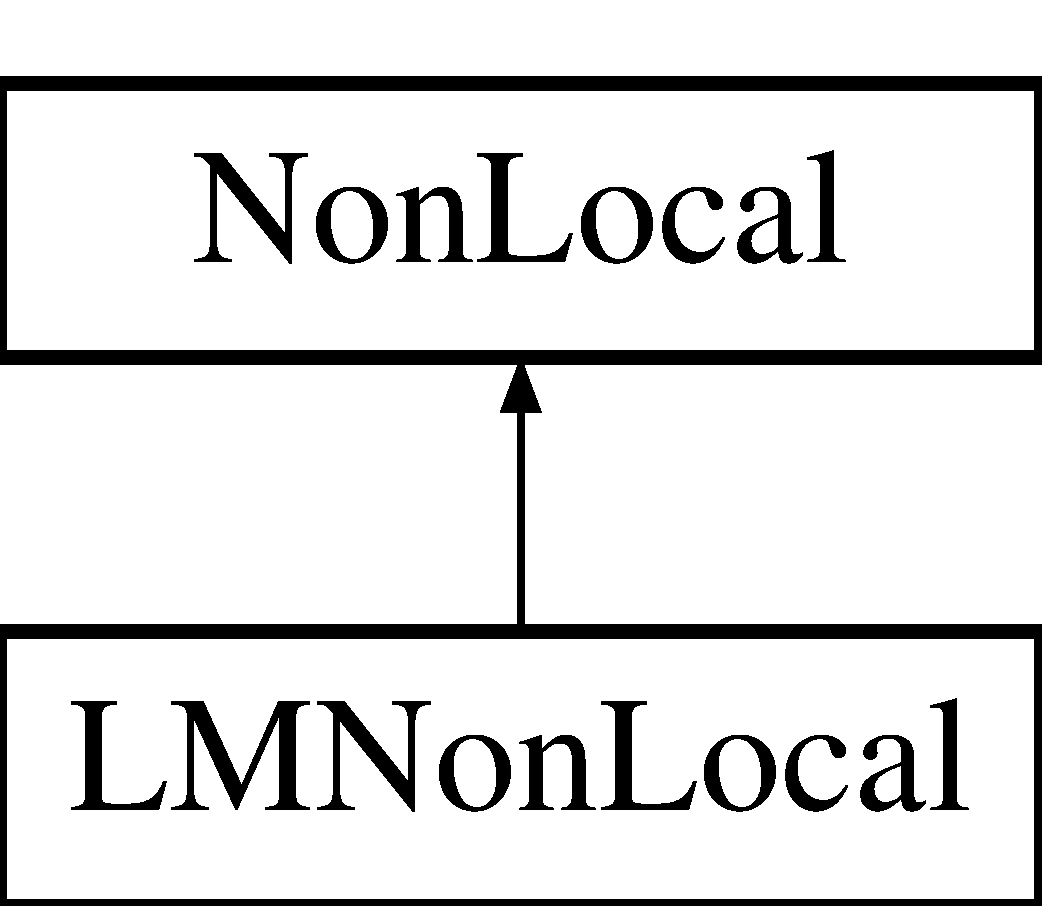
\includegraphics[height=2cm]{class_l_m_non_local}
\end{center}
\end{figure}
\subsection*{Public Member Functions}
\begin{DoxyCompactItemize}
\item 
\hypertarget{class_l_m_non_local_a7a6000f6118f1c8df727fac29c849b58}{
{\bfseries LMNonLocal} (const \hyperlink{class_scarab_1_1_h_g_1_1_h_graph}{HGraph} \&forest, Ngram \&lm, const \hyperlink{class_cache}{Cache}$<$ \hyperlink{class_scarab_1_1_h_g_1_1_hypernode}{Hypernode}, int $>$ \&word\_\-cache)}
\label{class_l_m_non_local_a7a6000f6118f1c8df727fac29c849b58}

\item 
\hypertarget{class_l_m_non_local_a2d14ca694dc6d49ce6e2b80622aafd51}{
void {\bfseries compute} (const \hyperlink{class_scarab_1_1_h_g_1_1_hyperedge}{Hyperedge} \&edge, const vector$<$ vector$<$ int $>$ $>$ \&subder, double \&score, vector$<$ int $>$ \&full\_\-derivation, vector$<$ int $>$ \&sig) const }
\label{class_l_m_non_local_a2d14ca694dc6d49ce6e2b80622aafd51}

\item 
\hypertarget{class_l_m_non_local_a93334d873bfe91d5357cbec933ec3ae9}{
\hyperlink{struct_hyp}{Hyp} {\bfseries initialize} (const \hyperlink{class_scarab_1_1_h_g_1_1_hypernode}{Hypernode} \&node) const }
\label{class_l_m_non_local_a93334d873bfe91d5357cbec933ec3ae9}

\end{DoxyCompactItemize}


The documentation for this class was generated from the following file:\begin{DoxyCompactItemize}
\item 
CubeLM.h\end{DoxyCompactItemize}

\hypertarget{struct_local_hyperedge}{
\section{LocalHyperedge Struct Reference}
\label{struct_local_hyperedge}\index{LocalHyperedge@{LocalHyperedge}}
}
\subsection*{Public Attributes}
\begin{DoxyCompactItemize}
\item 
\hypertarget{struct_local_hyperedge_a94cbc62434996702ca1d0e28b6dde622}{
vector$<$ int $>$ {\bfseries tail\_\-node\_\-ids}}
\label{struct_local_hyperedge_a94cbc62434996702ca1d0e28b6dde622}

\item 
\hypertarget{struct_local_hyperedge_a71c8831cc00fefbfb29575856a22fc8a}{
int {\bfseries head}}
\label{struct_local_hyperedge_a71c8831cc00fefbfb29575856a22fc8a}

\item 
\hypertarget{struct_local_hyperedge_a875e26d7749b13e387b7f0978a4f97a5}{
double {\bfseries weight}}
\label{struct_local_hyperedge_a875e26d7749b13e387b7f0978a4f97a5}

\item 
\hypertarget{struct_local_hyperedge_ae1b43e113b237128ed95691034ec715e}{
string {\bfseries label}}
\label{struct_local_hyperedge_ae1b43e113b237128ed95691034ec715e}

\end{DoxyCompactItemize}


The documentation for this struct was generated from the following file:\begin{DoxyCompactItemize}
\item 
parse/EisnerToHypergraph.h\end{DoxyCompactItemize}

\hypertarget{class_local_test_suite}{
\section{LocalTestSuite Class Reference}
\label{class_local_test_suite}\index{LocalTestSuite@{LocalTestSuite}}
}


The documentation for this class was generated from the following file:\begin{DoxyCompactItemize}
\item 
lattice/Test.cpp\end{DoxyCompactItemize}

\hypertarget{struct_scarab_1_1_h_g_1_1_location}{
\section{Scarab::HG::Location Struct Reference}
\label{struct_scarab_1_1_h_g_1_1_location}\index{Scarab::HG::Location@{Scarab::HG::Location}}
}
\subsection*{Public Member Functions}
\begin{DoxyCompactItemize}
\item 
\hypertarget{struct_scarab_1_1_h_g_1_1_location_a66e686eed3a0038886fd24171ec0ae8e}{
void {\bfseries show} ()}
\label{struct_scarab_1_1_h_g_1_1_location_a66e686eed3a0038886fd24171ec0ae8e}

\end{DoxyCompactItemize}
\subsection*{Public Attributes}
\begin{DoxyCompactItemize}
\item 
\hypertarget{struct_scarab_1_1_h_g_1_1_location_a493249f5c4c2ad6870d1cf1f9dd3f5f5}{
loc {\bfseries location}}
\label{struct_scarab_1_1_h_g_1_1_location_a493249f5c4c2ad6870d1cf1f9dd3f5f5}

\item 
\hypertarget{struct_scarab_1_1_h_g_1_1_location_a9a11d2d02ffd88048526a28c7619a3c7}{
int {\bfseries node\_\-id}}
\label{struct_scarab_1_1_h_g_1_1_location_a9a11d2d02ffd88048526a28c7619a3c7}

\item 
\hypertarget{struct_scarab_1_1_h_g_1_1_location_a618dd1682636ccc635ced4dc536be305}{
int {\bfseries edge\_\-id}}
\label{struct_scarab_1_1_h_g_1_1_location_a618dd1682636ccc635ced4dc536be305}

\item 
\hypertarget{struct_scarab_1_1_h_g_1_1_location_a9e3f8708a3b6c0271a7a854bc6dbde79}{
int {\bfseries edge\_\-pos}}
\label{struct_scarab_1_1_h_g_1_1_location_a9e3f8708a3b6c0271a7a854bc6dbde79}

\end{DoxyCompactItemize}


The documentation for this struct was generated from the following file:\begin{DoxyCompactItemize}
\item 
hypergraph/AStar.h\end{DoxyCompactItemize}

\hypertarget{class_scarab_1_1_h_g_1_1_l_p_builder}{
\section{Scarab::HG::LPBuilder Class Reference}
\label{class_scarab_1_1_h_g_1_1_l_p_builder}\index{Scarab::HG::LPBuilder@{Scarab::HG::LPBuilder}}
}
\subsection*{Public Member Functions}
\begin{DoxyCompactItemize}
\item 
\hypertarget{class_scarab_1_1_h_g_1_1_l_p_builder_aba798e4d3faf87e8411607f9d974fc7f}{
{\bfseries LPBuilder} (const \hyperlink{class_scarab_1_1_h_g_1_1_h_graph}{HGraph} \&forest, const \hyperlink{class_forest_lattice}{ForestLattice} \&lat)}
\label{class_scarab_1_1_h_g_1_1_l_p_builder_aba798e4d3faf87e8411607f9d974fc7f}

\item 
\hypertarget{class_scarab_1_1_h_g_1_1_l_p_builder_abfa755f4c94dc432c022be35861a8200}{
void {\bfseries solve\_\-hypergraph} (const \hyperlink{class_cache}{Cache}$<$ \hyperlink{class_scarab_1_1_h_g_1_1_hyperedge}{Hyperedge}, double $>$ \&)}
\label{class_scarab_1_1_h_g_1_1_l_p_builder_abfa755f4c94dc432c022be35861a8200}

\item 
\hypertarget{class_scarab_1_1_h_g_1_1_l_p_builder_a963bdf9c956b4a08d52be06e1cb6a05a}{
void {\bfseries solve\_\-full} (int run\_\-num, const \hyperlink{class_cache}{Cache}$<$ \hyperlink{class_scarab_1_1_h_g_1_1_hyperedge}{Hyperedge}, double $>$ \&\_\-weights, Ngram \&lm, const \hyperlink{class_cache}{Cache}$<$ \hyperlink{class_scarab_1_1_graph_1_1_graphnode}{Graphnode}, int $>$ \&word\_\-cache)}
\label{class_scarab_1_1_h_g_1_1_l_p_builder_a963bdf9c956b4a08d52be06e1cb6a05a}

\end{DoxyCompactItemize}


The documentation for this class was generated from the following files:\begin{DoxyCompactItemize}
\item 
lp/LPBuilder.h\item 
lp/LPBuilder.cpp\end{DoxyCompactItemize}

\hypertarget{class_m_r_f}{
\section{MRF Class Reference}
\label{class_m_r_f}\index{MRF@{MRF}}
}
Inheritance diagram for MRF:\begin{figure}[H]
\begin{center}
\leavevmode
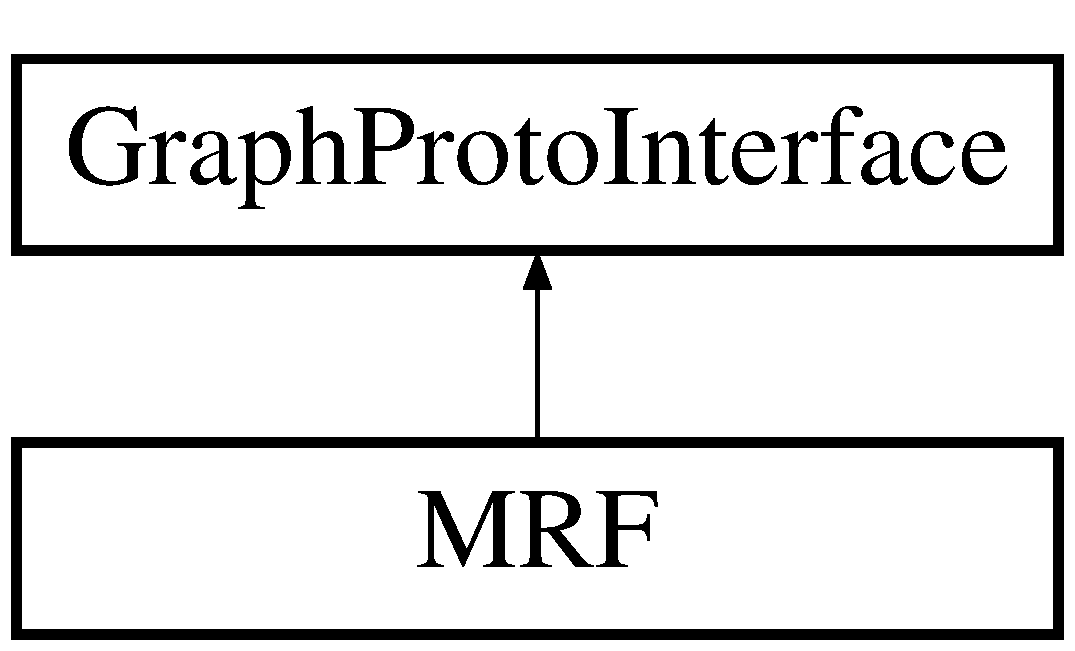
\includegraphics[height=2cm]{class_m_r_f}
\end{center}
\end{figure}
\subsection*{Public Member Functions}
\begin{DoxyCompactItemize}
\item 
\hypertarget{class_m_r_f_a3a2f7eb349a7345abfba2c5869f85b1f}{
void {\bfseries process\_\-node} (graph::Graph\_\-Node, \hyperlink{class_scarab_1_1_graph_1_1_graphnode}{Graphnode} $\ast$)}
\label{class_m_r_f_a3a2f7eb349a7345abfba2c5869f85b1f}

\item 
\hypertarget{class_m_r_f_aed7b8a7a2e3af7c14b501040630e9589}{
void {\bfseries process\_\-edge} (graph::Graph\_\-Edge, \hyperlink{class_scarab_1_1_graph_1_1_graphedge}{Graphedge} $\ast$)}
\label{class_m_r_f_aed7b8a7a2e3af7c14b501040630e9589}

\item 
\hypertarget{class_m_r_f_a34f0d586337501d668a62726eb0046d7}{
Hypergraph $\ast$ {\bfseries build\_\-hypergraph} ()}
\label{class_m_r_f_a34f0d586337501d668a62726eb0046d7}

\item 
void \hyperlink{class_m_r_f_a928f19f948fa97796462fd9542a985fd}{set\_\-up} (graph::Graph graph, int nodes, int edges)
\item 
\hypertarget{class_m_r_f_a3a7f11091d96ab8b2f830deb343fc3a6}{
const double {\bfseries node\_\-pot} (const \hyperlink{class_scarab_1_1_graph_1_1_graphnode}{Graphnode} \&node, const \hyperlink{struct_state}{State} \&s1) const }
\label{class_m_r_f_a3a7f11091d96ab8b2f830deb343fc3a6}

\item 
\hypertarget{class_m_r_f_ab73d5f7b51c206754bee9eea9405c0fb}{
const bool {\bfseries has\_\-edge\_\-pot} (const \hyperlink{class_scarab_1_1_graph_1_1_graphedge}{Graphedge} \&edge, const \hyperlink{struct_state}{State} \&s1, const \hyperlink{struct_state}{State} \&s2) const }
\label{class_m_r_f_ab73d5f7b51c206754bee9eea9405c0fb}

\item 
\hypertarget{class_m_r_f_a9f98956295352e9bfc9917328999c1b2}{
const double {\bfseries edge\_\-pot} (const \hyperlink{class_scarab_1_1_graph_1_1_graphedge}{Graphedge} \&edge, const \hyperlink{struct_state}{State} \&s1, const \hyperlink{struct_state}{State} \&s2) const }
\label{class_m_r_f_a9f98956295352e9bfc9917328999c1b2}

\item 
\hypertarget{class_m_r_f_a7c01a68384b81d1ba7d24508f767d216}{
const vector$<$ \hyperlink{struct_state}{State} $>$ \& {\bfseries states} (const \hyperlink{class_scarab_1_1_graph_1_1_graphnode}{Graphnode} \&node) const }
\label{class_m_r_f_a7c01a68384b81d1ba7d24508f767d216}

\item 
\hypertarget{class_m_r_f_aaf17c4a671ea4f06553c33fca90bfa35}{
const int {\bfseries assignments} () const }
\label{class_m_r_f_aaf17c4a671ea4f06553c33fca90bfa35}

\item 
\hypertarget{class_m_r_f_a9326b3fd5aea915a1bb8a1ad2ac50f3f}{
\hyperlink{struct_node_assignment}{NodeAssignment} {\bfseries make\_\-assignment} (const \hyperlink{class_scarab_1_1_graph_1_1_graphnode}{Graphnode} \&n, const \hyperlink{struct_state}{State} \&my\_\-s) const }
\label{class_m_r_f_a9326b3fd5aea915a1bb8a1ad2ac50f3f}

\end{DoxyCompactItemize}


\subsection{Member Function Documentation}
\hypertarget{class_m_r_f_a928f19f948fa97796462fd9542a985fd}{
\index{MRF@{MRF}!set\_\-up@{set\_\-up}}
\index{set\_\-up@{set\_\-up}!MRF@{MRF}}
\subsubsection[{set\_\-up}]{\setlength{\rightskip}{0pt plus 5cm}void MRF::set\_\-up (graph::Graph {\em graph}, \/  int {\em nodes}, \/  int {\em edges})\hspace{0.3cm}{\ttfamily  \mbox{[}virtual\mbox{]}}}}
\label{class_m_r_f_a928f19f948fa97796462fd9542a985fd}
Solve the potts model with the given node potentials


\begin{DoxyParams}{Parameters}
\item[{\em node\_\-potentials}]\end{DoxyParams}


Reimplemented from \hyperlink{class_graph_proto_interface}{GraphProtoInterface}.



The documentation for this class was generated from the following files:\begin{DoxyCompactItemize}
\item 
optimization/MRF.h\item 
optimization/MRF.cpp\end{DoxyCompactItemize}

\hypertarget{class_m_r_f_builder_l_p}{
\section{MRFBuilderLP Class Reference}
\label{class_m_r_f_builder_l_p}\index{MRFBuilderLP@{MRFBuilderLP}}
}
\subsection*{Static Public Member Functions}
\begin{DoxyCompactItemize}
\item 
\hypertarget{class_m_r_f_builder_l_p_aaace30ed1c0dfb1b0c5c89a22b503e10}{
static \hyperlink{struct_m_r_f_l_p}{MRFLP} $\ast$ {\bfseries add\_\-mrf} (const \hyperlink{class_m_r_f}{MRF} \&mrf, string prefix, GRBModel \&model, int var\_\-type)}
\label{class_m_r_f_builder_l_p_aaace30ed1c0dfb1b0c5c89a22b503e10}

\end{DoxyCompactItemize}


The documentation for this class was generated from the following files:\begin{DoxyCompactItemize}
\item 
lp/MRFLP.h\item 
lp/MRFLP.cpp\end{DoxyCompactItemize}

\hypertarget{class_m_r_f_hypergraph}{
\section{MRFHypergraph Class Reference}
\label{class_m_r_f_hypergraph}\index{MRFHypergraph@{MRFHypergraph}}
}
Inheritance diagram for MRFHypergraph:\begin{figure}[H]
\begin{center}
\leavevmode
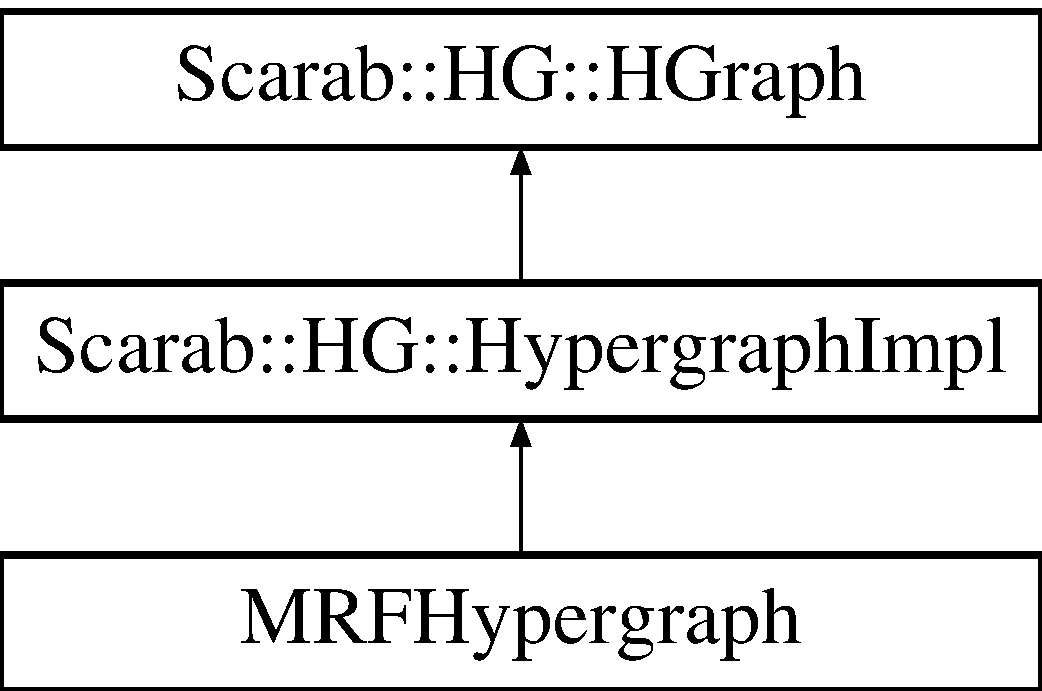
\includegraphics[height=3cm]{class_m_r_f_hypergraph}
\end{center}
\end{figure}
\subsection*{Public Member Functions}
\begin{DoxyCompactItemize}
\item 
\hypertarget{class_m_r_f_hypergraph_a5c717b35842c25c6be9e827f0aa31708}{
\hyperlink{struct_node_assignment}{NodeAssignment} {\bfseries assignment\_\-from\_\-node} (\hyperlink{class_scarab_1_1_h_g_1_1_hypernode}{Hypernode} $\ast$node)}
\label{class_m_r_f_hypergraph_a5c717b35842c25c6be9e827f0aa31708}

\item 
void \hyperlink{class_m_r_f_hypergraph_aaac6b68c3ece41ddd1f8107e961879bc}{print} () const 
\item 
\hypertarget{class_m_r_f_hypergraph_a34f14a3a9cf0d01c7fbfc11e1caa20ba}{
\hyperlink{class_scarab_1_1_h_g_1_1_hypernode}{HNode} {\bfseries assignment\_\-from\_\-node} (\hyperlink{struct_node_assignment}{NodeAssignment} \&node\_\-assign)}
\label{class_m_r_f_hypergraph_a34f14a3a9cf0d01c7fbfc11e1caa20ba}

\end{DoxyCompactItemize}
\subsection*{Static Public Member Functions}
\begin{DoxyCompactItemize}
\item 
\hypertarget{class_m_r_f_hypergraph_af8808e644c7ff0c938f4fbd9e473dfba}{
static \hyperlink{class_m_r_f_hypergraph}{MRFHypergraph} {\bfseries from\_\-mrf} (const \hyperlink{class_m_r_f}{MRF} \&mrf)}
\label{class_m_r_f_hypergraph_af8808e644c7ff0c938f4fbd9e473dfba}

\end{DoxyCompactItemize}


\subsection{Member Function Documentation}
\hypertarget{class_m_r_f_hypergraph_aaac6b68c3ece41ddd1f8107e961879bc}{
\index{MRFHypergraph@{MRFHypergraph}!print@{print}}
\index{print@{print}!MRFHypergraph@{MRFHypergraph}}
\subsubsection[{print}]{\setlength{\rightskip}{0pt plus 5cm}void MRFHypergraph::print () const\hspace{0.3cm}{\ttfamily  \mbox{[}inline, virtual\mbox{]}}}}
\label{class_m_r_f_hypergraph_aaac6b68c3ece41ddd1f8107e961879bc}
Display the hypergraph for debugging. 

Implements \hyperlink{class_scarab_1_1_h_g_1_1_h_graph_ab5aa11c932b28864b56f28e0babbc1c1}{Scarab::HG::HGraph}.



The documentation for this class was generated from the following files:\begin{DoxyCompactItemize}
\item 
optimization/MRFHypergraph.h\item 
optimization/MRFHypergraph.cpp\end{DoxyCompactItemize}

\hypertarget{struct_mrf_index}{
\section{MrfIndex Struct Reference}
\label{struct_mrf_index}\index{MrfIndex@{MrfIndex}}
}
\subsection*{Public Member Functions}
\begin{DoxyCompactItemize}
\item 
\hypertarget{struct_mrf_index_adc62126e39eeccb67aed83b8d33514e9}{
{\bfseries MrfIndex} (int group\_\-, int node\_\-, int state\_\-)}
\label{struct_mrf_index_adc62126e39eeccb67aed83b8d33514e9}

\end{DoxyCompactItemize}
\subsection*{Public Attributes}
\begin{DoxyCompactItemize}
\item 
\hypertarget{struct_mrf_index_a10be38457b3798cfdf70f224814ce8eb}{
int {\bfseries group}}
\label{struct_mrf_index_a10be38457b3798cfdf70f224814ce8eb}

\item 
\hypertarget{struct_mrf_index_a9c765fbc8576d8d6541a072eb75c2c8a}{
int {\bfseries node}}
\label{struct_mrf_index_a9c765fbc8576d8d6541a072eb75c2c8a}

\item 
\hypertarget{struct_mrf_index_a2cea032a5c169945c3c0e8d96fbc1477}{
int {\bfseries state}}
\label{struct_mrf_index_a2cea032a5c169945c3c0e8d96fbc1477}

\end{DoxyCompactItemize}


The documentation for this struct was generated from the following file:\begin{DoxyCompactItemize}
\item 
tagger/TagConstraints.h\end{DoxyCompactItemize}

\hypertarget{struct_m_r_f_l_p}{
\section{MRFLP Struct Reference}
\label{struct_m_r_f_l_p}\index{MRFLP@{MRFLP}}
}
\subsection*{Public Member Functions}
\begin{DoxyCompactItemize}
\item 
\hypertarget{struct_m_r_f_l_p_a868a64efdbf8d42682c7953361af4c31}{
{\bfseries MRFLP} (const \hyperlink{class_m_r_f}{MRF} \&p)}
\label{struct_m_r_f_l_p_a868a64efdbf8d42682c7953361af4c31}

\end{DoxyCompactItemize}
\subsection*{Public Attributes}
\begin{DoxyCompactItemize}
\item 
\hypertarget{struct_m_r_f_l_p_a1ddb2cc0eb980dc0d9d94bf731e3f4ae}{
\hyperlink{class_cache}{Cache}$<$ \hyperlink{class_scarab_1_1_graph_1_1_graphnode}{Graphnode}, \hyperlink{class_cache}{Cache}$<$ \hyperlink{struct_state}{State}, GRBVar $>$ $\ast$ $>$ {\bfseries node\_\-vars}}
\label{struct_m_r_f_l_p_a1ddb2cc0eb980dc0d9d94bf731e3f4ae}

\item 
\hypertarget{struct_m_r_f_l_p_a7f977d31ba7f70b5913279466a46e2b2}{
\hyperlink{class_cache}{Cache}$<$ \hyperlink{class_scarab_1_1_graph_1_1_graphedge}{Graphedge}, \hyperlink{class_cache}{Cache}$<$ \hyperlink{struct_state}{State}, \hyperlink{class_cache}{Cache}$<$ \hyperlink{struct_state}{State}, GRBVar $>$ $\ast$ $>$ $\ast$ $>$ {\bfseries edge\_\-vars}}
\label{struct_m_r_f_l_p_a7f977d31ba7f70b5913279466a46e2b2}

\item 
\hypertarget{struct_m_r_f_l_p_a46a1042ee20d632ca11afee0a1965fb9}{
\hyperlink{class_cache}{Cache}$<$ \hyperlink{class_scarab_1_1_graph_1_1_graphedge}{Graphedge}, \hyperlink{class_cache}{Cache}$<$ \hyperlink{struct_state}{State}, GRBVar $>$ $\ast$ $>$ {\bfseries from\_\-state\_\-blank\_\-vars}}
\label{struct_m_r_f_l_p_a46a1042ee20d632ca11afee0a1965fb9}

\item 
\hypertarget{struct_m_r_f_l_p_ae1b4c653d4a3b3c6759a160f8f1c4fc6}{
\hyperlink{class_cache}{Cache}$<$ \hyperlink{class_scarab_1_1_graph_1_1_graphedge}{Graphedge}, \hyperlink{class_cache}{Cache}$<$ \hyperlink{struct_state}{State}, GRBVar $>$ $\ast$ $>$ {\bfseries to\_\-state\_\-blank\_\-vars}}
\label{struct_m_r_f_l_p_ae1b4c653d4a3b3c6759a160f8f1c4fc6}

\item 
\hypertarget{struct_m_r_f_l_p_a546b7ee8de350e2a882e9ae9beb6af6f}{
const \hyperlink{class_m_r_f}{MRF} \& {\bfseries mrf}}
\label{struct_m_r_f_l_p_a546b7ee8de350e2a882e9ae9beb6af6f}

\end{DoxyCompactItemize}


The documentation for this struct was generated from the following file:\begin{DoxyCompactItemize}
\item 
lp/MRFLP.h\end{DoxyCompactItemize}

\hypertarget{class_ngram_cache}{
\section{NgramCache Class Reference}
\label{class_ngram_cache}\index{NgramCache@{NgramCache}}
}
\subsection*{Public Member Functions}
\begin{DoxyCompactItemize}
\item 
\hypertarget{class_ngram_cache_a1d8b66016081c1e0d15b2199e48c4df9}{
{\bfseries NgramCache} (Vocab \&v, int i)}
\label{class_ngram_cache_a1d8b66016081c1e0d15b2199e48c4df9}

\item 
\hypertarget{class_ngram_cache_aaf831fb4e48aa1a8f8d46287adb7c419}{
bool {\bfseries hasNext} (const VocabIndex next)}
\label{class_ngram_cache_aaf831fb4e48aa1a8f8d46287adb7c419}

\item 
\hypertarget{class_ngram_cache_a3444ab6a1b5a140edb089efb51b071c1}{
LogP {\bfseries wordProbPrimeCache} (VocabIndex word, const VocabIndex $\ast$context)}
\label{class_ngram_cache_a3444ab6a1b5a140edb089efb51b071c1}

\item 
\hypertarget{class_ngram_cache_a7806b0a2832644fcde66aa928a58caa9}{
LogP {\bfseries wordProbFromCache} (VocabIndex word, const VocabIndex $\ast$context)}
\label{class_ngram_cache_a7806b0a2832644fcde66aa928a58caa9}

\end{DoxyCompactItemize}


The documentation for this class was generated from the following files:\begin{DoxyCompactItemize}
\item 
trans\_\-decode/NGramCache.h\item 
trans\_\-decode/NGramCache.cpp\end{DoxyCompactItemize}

\hypertarget{struct_node_assignment}{
\section{NodeAssignment Struct Reference}
\label{struct_node_assignment}\index{NodeAssignment@{NodeAssignment}}
}
\subsection*{Public Member Functions}
\begin{DoxyCompactItemize}
\item 
\hypertarget{struct_node_assignment_afb4f063136a9da957865d42faa2a3943}{
{\bfseries NodeAssignment} (int node\_\-id\_\-, const \hyperlink{struct_state}{State} state\_\-, int length\_\-)}
\label{struct_node_assignment_afb4f063136a9da957865d42faa2a3943}

\item 
\hypertarget{struct_node_assignment_aea41536d91eba4d9c6440065953aa4e0}{
int {\bfseries id} () const }
\label{struct_node_assignment_aea41536d91eba4d9c6440065953aa4e0}

\end{DoxyCompactItemize}
\subsection*{Public Attributes}
\begin{DoxyCompactItemize}
\item 
\hypertarget{struct_node_assignment_a595045041aa245ed3108284223ce766d}{
int {\bfseries node\_\-id}}
\label{struct_node_assignment_a595045041aa245ed3108284223ce766d}

\item 
\hypertarget{struct_node_assignment_affe9bfbc195ba56f34dcdbd4fb10411e}{
\hyperlink{struct_state}{State} {\bfseries s}}
\label{struct_node_assignment_affe9bfbc195ba56f34dcdbd4fb10411e}

\item 
\hypertarget{struct_node_assignment_ac3b88ac2cbd270733ee835e00279a4ad}{
int {\bfseries length}}
\label{struct_node_assignment_ac3b88ac2cbd270733ee835e00279a4ad}

\end{DoxyCompactItemize}


The documentation for this struct was generated from the following file:\begin{DoxyCompactItemize}
\item 
optimization/MRF.h\end{DoxyCompactItemize}

\hypertarget{class_non_local}{
\section{NonLocal Class Reference}
\label{class_non_local}\index{NonLocal@{NonLocal}}
}
Inheritance diagram for NonLocal:\begin{figure}[H]
\begin{center}
\leavevmode
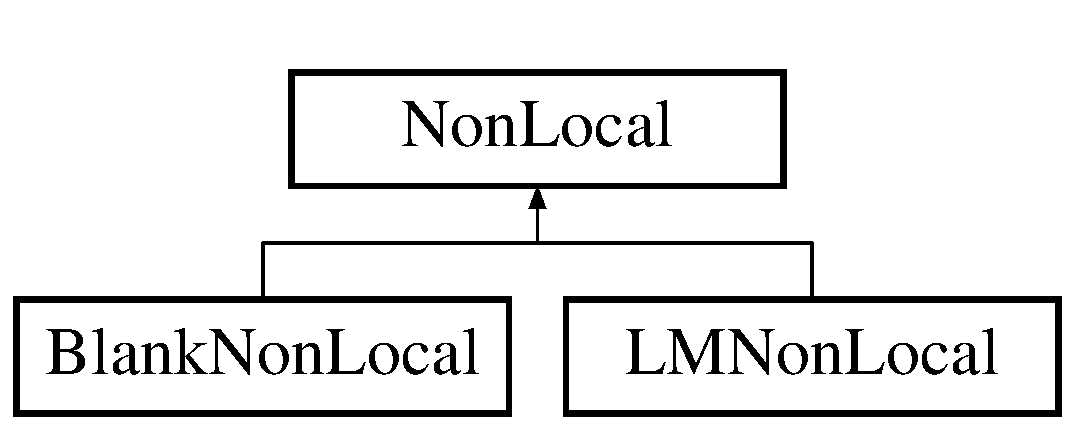
\includegraphics[height=2cm]{class_non_local}
\end{center}
\end{figure}
\subsection*{Public Member Functions}
\begin{DoxyCompactItemize}
\item 
\hypertarget{class_non_local_acd66e7882a5bb3415d3fd658d03ec8fc}{
virtual void {\bfseries compute} (const \hyperlink{class_scarab_1_1_h_g_1_1_hyperedge}{Hyperedge} \&, const vector$<$ vector$<$ int $>$ $>$ \&, double \&score, vector$<$ int $>$ \&full\_\-derivation, Sig \&sig) const =0}
\label{class_non_local_acd66e7882a5bb3415d3fd658d03ec8fc}

\item 
\hypertarget{class_non_local_a90f2d399853f5c689a0abdc5c12a8370}{
virtual \hyperlink{struct_hyp}{Hyp} {\bfseries initialize} (const \hyperlink{class_scarab_1_1_h_g_1_1_hypernode}{Hypernode} \&) const =0}
\label{class_non_local_a90f2d399853f5c689a0abdc5c12a8370}

\end{DoxyCompactItemize}


The documentation for this class was generated from the following file:\begin{DoxyCompactItemize}
\item 
hypergraph/CubePruning.h\end{DoxyCompactItemize}

\hypertarget{class_phrase_based}{
\section{PhraseBased Class Reference}
\label{class_phrase_based}\index{PhraseBased@{PhraseBased}}
}
Inheritance diagram for PhraseBased:\begin{figure}[H]
\begin{center}
\leavevmode
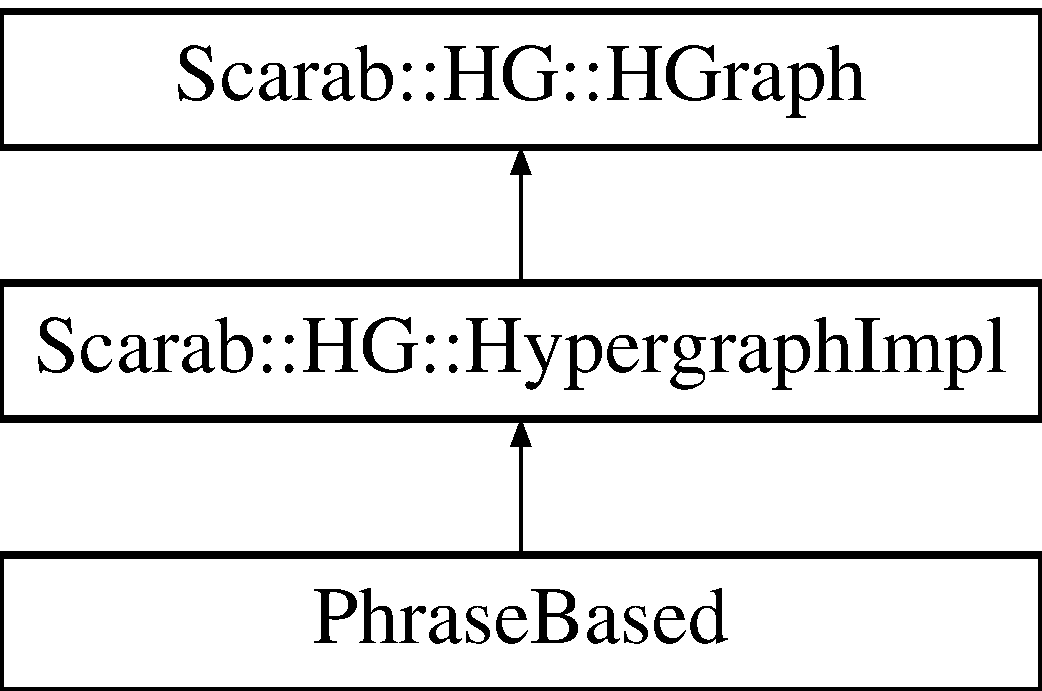
\includegraphics[height=3cm]{class_phrase_based}
\end{center}
\end{figure}
\subsection*{Public Member Functions}
\begin{DoxyCompactItemize}
\item 
void \hyperlink{class_phrase_based_aafc2997b58b3698fed7cb5a1f6f269c6}{print} () const 
\item 
\hypertarget{class_phrase_based_a3883660c72be6ce8daab08f368317853}{
void {\bfseries set\_\-up} (const Hypergraph \&hgraph)}
\label{class_phrase_based_a3883660c72be6ce8daab08f368317853}

\end{DoxyCompactItemize}


\subsection{Member Function Documentation}
\hypertarget{class_phrase_based_aafc2997b58b3698fed7cb5a1f6f269c6}{
\index{PhraseBased@{PhraseBased}!print@{print}}
\index{print@{print}!PhraseBased@{PhraseBased}}
\subsubsection[{print}]{\setlength{\rightskip}{0pt plus 5cm}void PhraseBased::print () const\hspace{0.3cm}{\ttfamily  \mbox{[}inline, virtual\mbox{]}}}}
\label{class_phrase_based_aafc2997b58b3698fed7cb5a1f6f269c6}
Display the hypergraph for debugging. 

Implements \hyperlink{class_scarab_1_1_h_g_1_1_h_graph_ab5aa11c932b28864b56f28e0babbc1c1}{Scarab::HG::HGraph}.



The documentation for this class was generated from the following file:\begin{DoxyCompactItemize}
\item 
phrasebased/PhraseBased.h\end{DoxyCompactItemize}

\hypertarget{struct_possible_dep}{
\section{PossibleDep Struct Reference}
\label{struct_possible_dep}\index{PossibleDep@{PossibleDep}}
}
\subsection*{Public Attributes}
\begin{DoxyCompactItemize}
\item 
\hypertarget{struct_possible_dep_a2f693c6bb47703c1a989f8971e06d561}{
int {\bfseries ind}}
\label{struct_possible_dep_a2f693c6bb47703c1a989f8971e06d561}

\item 
\hypertarget{struct_possible_dep_ad2c0887a242af14d7bdd6bc7a3528bf3}{
int {\bfseries group}}
\label{struct_possible_dep_ad2c0887a242af14d7bdd6bc7a3528bf3}

\item 
\hypertarget{struct_possible_dep_a2f685f514a785a8365c9a1682fce4d5a}{
string {\bfseries group\_\-name}}
\label{struct_possible_dep_a2f685f514a785a8365c9a1682fce4d5a}

\item 
\hypertarget{struct_possible_dep_a4b4536449d9c17e05b7f5454b0d922f7}{
vector$<$ int $>$ {\bfseries head\_\-inds}}
\label{struct_possible_dep_a4b4536449d9c17e05b7f5454b0d922f7}

\item 
\hypertarget{struct_possible_dep_acec0859157184e3f1fe962236fe6303b}{
int {\bfseries sent\_\-num}}
\label{struct_possible_dep_acec0859157184e3f1fe962236fe6303b}

\end{DoxyCompactItemize}


The documentation for this struct was generated from the following file:\begin{DoxyCompactItemize}
\item 
lp/HardConstraints.h\end{DoxyCompactItemize}

\hypertarget{struct_possible_tag}{
\section{PossibleTag Struct Reference}
\label{struct_possible_tag}\index{PossibleTag@{PossibleTag}}
}
\subsection*{Public Member Functions}
\begin{DoxyCompactItemize}
\item 
\hypertarget{struct_possible_tag_a63f51fa07de58355955633c1fc5ec5c7}{
int {\bfseries weight\_\-id} (POS tag) const }
\label{struct_possible_tag_a63f51fa07de58355955633c1fc5ec5c7}

\item 
\hypertarget{struct_possible_tag_a83442edca34aefb4376d36dee744a28b}{
bool {\bfseries operator$<$} (const \hyperlink{struct_possible_tag}{PossibleTag} \&other) const }
\label{struct_possible_tag_a83442edca34aefb4376d36dee744a28b}

\end{DoxyCompactItemize}
\subsection*{Public Attributes}
\begin{DoxyCompactItemize}
\item 
\hypertarget{struct_possible_tag_a8c69b59e1e75a5f80623cce26baacabb}{
int {\bfseries id}}
\label{struct_possible_tag_a8c69b59e1e75a5f80623cce26baacabb}

\item 
\hypertarget{struct_possible_tag_a822aff1087d9f91882bf45da7f129e75}{
int {\bfseries ind}}
\label{struct_possible_tag_a822aff1087d9f91882bf45da7f129e75}

\item 
\hypertarget{struct_possible_tag_a26244f2c445f233652e4c3ffebafa894}{
int {\bfseries sent\_\-num}}
\label{struct_possible_tag_a26244f2c445f233652e4c3ffebafa894}

\item 
\hypertarget{struct_possible_tag_a25eb72efa84dc8e030a928c091391609}{
int {\bfseries group}}
\label{struct_possible_tag_a25eb72efa84dc8e030a928c091391609}

\item 
\hypertarget{struct_possible_tag_afcfa2ffd67a92a564d5c16aa3945b8a0}{
string {\bfseries group\_\-name}}
\label{struct_possible_tag_afcfa2ffd67a92a564d5c16aa3945b8a0}

\item 
\hypertarget{struct_possible_tag_adc65412fc67deda1ac5554fdbb0264d2}{
int {\bfseries training\_\-count}}
\label{struct_possible_tag_adc65412fc67deda1ac5554fdbb0264d2}

\item 
\hypertarget{struct_possible_tag_ae933b21144c99f1197a5254e8ceb1c7c}{
int {\bfseries test\_\-count}}
\label{struct_possible_tag_ae933b21144c99f1197a5254e8ceb1c7c}

\end{DoxyCompactItemize}


The documentation for this struct was generated from the following file:\begin{DoxyCompactItemize}
\item 
tagger/TagConstraints.h\end{DoxyCompactItemize}

\hypertarget{class_potts_model_builder_l_p}{
\section{PottsModelBuilderLP Class Reference}
\label{class_potts_model_builder_l_p}\index{PottsModelBuilderLP@{PottsModelBuilderLP}}
}
\subsection*{Static Public Member Functions}
\begin{DoxyCompactItemize}
\item 
\hypertarget{class_potts_model_builder_l_p_af62f78dc2bdeb5b4d39444c47f8ad341}{
static \hyperlink{struct_potts_model_l_p}{PottsModelLP} $\ast$ {\bfseries add\_\-potts} (const PottsModel \&potts, GRBModel \&model, int var\_\-type)}
\label{class_potts_model_builder_l_p_af62f78dc2bdeb5b4d39444c47f8ad341}

\end{DoxyCompactItemize}


The documentation for this class was generated from the following file:\begin{DoxyCompactItemize}
\item 
lp/PottsModelLP.h\end{DoxyCompactItemize}

\hypertarget{struct_potts_model_l_p}{
\section{PottsModelLP Struct Reference}
\label{struct_potts_model_l_p}\index{PottsModelLP@{PottsModelLP}}
}
\subsection*{Public Member Functions}
\begin{DoxyCompactItemize}
\item 
\hypertarget{struct_potts_model_l_p_af041b236eacf847879e1a2ba53b6e987}{
{\bfseries PottsModelLP} (const PottsModel \&p)}
\label{struct_potts_model_l_p_af041b236eacf847879e1a2ba53b6e987}

\end{DoxyCompactItemize}
\subsection*{Public Attributes}
\begin{DoxyCompactItemize}
\item 
\hypertarget{struct_potts_model_l_p_ac572d15bc61963f636a39e752951cf31}{
\hyperlink{class_cache}{Cache}$<$ Graphnode, \hyperlink{class_cache}{Cache}$<$ \hyperlink{struct_state}{State}, GRBVar $>$ $\ast$ $>$ {\bfseries node\_\-vars}}
\label{struct_potts_model_l_p_ac572d15bc61963f636a39e752951cf31}

\item 
\hypertarget{struct_potts_model_l_p_a00e3418b717ea5c1a0334dc30dafcdcc}{
\hyperlink{class_cache}{Cache}$<$ Graphedge, \hyperlink{class_cache}{Cache}$<$ \hyperlink{struct_state}{State}, \hyperlink{class_cache}{Cache}$<$ \hyperlink{struct_state}{State}, GRBVar $>$ $\ast$ $>$ $\ast$ $>$ {\bfseries edge\_\-vars}}
\label{struct_potts_model_l_p_a00e3418b717ea5c1a0334dc30dafcdcc}

\item 
\hypertarget{struct_potts_model_l_p_ad829fe7b19ca64ae117303082784d110}{
const PottsModel \& {\bfseries potts}}
\label{struct_potts_model_l_p_ad829fe7b19ca64ae117303082784d110}

\end{DoxyCompactItemize}


The documentation for this struct was generated from the following file:\begin{DoxyCompactItemize}
\item 
lp/PottsModelLP.h\end{DoxyCompactItemize}

\hypertarget{struct_scarab_1_1_h_g_1_1_queue_hyp}{
\section{Scarab::HG::QueueHyp Struct Reference}
\label{struct_scarab_1_1_h_g_1_1_queue_hyp}\index{Scarab::HG::QueueHyp@{Scarab::HG::QueueHyp}}
}
\subsection*{Public Member Functions}
\begin{DoxyCompactItemize}
\item 
\hypertarget{struct_scarab_1_1_h_g_1_1_queue_hyp_a165e60736b23d97bec8cdaff7c742db7}{
{\bfseries QueueHyp} (\hyperlink{struct_scarab_1_1_h_g_1_1_hypothesis}{Hypothesis} $\ast$hyp, double score\_\-in, \hyperlink{struct_scarab_1_1_h_g_1_1_location}{Location} $\ast$w)}
\label{struct_scarab_1_1_h_g_1_1_queue_hyp_a165e60736b23d97bec8cdaff7c742db7}

\item 
\hypertarget{struct_scarab_1_1_h_g_1_1_queue_hyp_aa02f7835d0dd0d00cc5f00ff7430ddf3}{
bool {\bfseries operator$<$} (const \hyperlink{struct_scarab_1_1_h_g_1_1_queue_hyp}{QueueHyp} \&other) const }
\label{struct_scarab_1_1_h_g_1_1_queue_hyp_aa02f7835d0dd0d00cc5f00ff7430ddf3}

\end{DoxyCompactItemize}
\subsection*{Public Attributes}
\begin{DoxyCompactItemize}
\item 
\hypertarget{struct_scarab_1_1_h_g_1_1_queue_hyp_ae3368ba62dae4842a83766b44bcda346}{
\hyperlink{struct_scarab_1_1_h_g_1_1_hypothesis}{Hypothesis} $\ast$ {\bfseries h}}
\label{struct_scarab_1_1_h_g_1_1_queue_hyp_ae3368ba62dae4842a83766b44bcda346}

\item 
\hypertarget{struct_scarab_1_1_h_g_1_1_queue_hyp_ab4c4483fa92ecb415def41f5ed366e53}{
double {\bfseries score}}
\label{struct_scarab_1_1_h_g_1_1_queue_hyp_ab4c4483fa92ecb415def41f5ed366e53}

\item 
\hypertarget{struct_scarab_1_1_h_g_1_1_queue_hyp_ae151535de5fa3bb2cfe44dade082c613}{
\hyperlink{struct_scarab_1_1_h_g_1_1_location}{Location} $\ast$ {\bfseries where}}
\label{struct_scarab_1_1_h_g_1_1_queue_hyp_ae151535de5fa3bb2cfe44dade082c613}

\end{DoxyCompactItemize}


The documentation for this struct was generated from the following file:\begin{DoxyCompactItemize}
\item 
hypergraph/AStar.h\end{DoxyCompactItemize}

\hypertarget{struct_span}{
\section{Span Struct Reference}
\label{struct_span}\index{Span@{Span}}
}
\subsection*{Public Member Functions}
\begin{DoxyCompactItemize}
\item 
\hypertarget{struct_span_aa5fb6e25d5c38cd540cc82ca179c82f2}{
{\bfseries Span} (int s, int e)}
\label{struct_span_aa5fb6e25d5c38cd540cc82ca179c82f2}

\item 
\hypertarget{struct_span_af6e7cf8f52e52996cf52bd7d702e9744}{
string {\bfseries name} ()}
\label{struct_span_af6e7cf8f52e52996cf52bd7d702e9744}

\item 
\hypertarget{struct_span_acebe6ab7baeb922c9c69aac317bbcb7a}{
bool {\bfseries operator==} (const \hyperlink{struct_span}{Span} \&other) const }
\label{struct_span_acebe6ab7baeb922c9c69aac317bbcb7a}

\item 
\hypertarget{struct_span_a413ed85231167a494dafeaea71fb4ae0}{
bool {\bfseries operator$<$} (const \hyperlink{struct_span}{Span} \&other) const }
\label{struct_span_a413ed85231167a494dafeaea71fb4ae0}

\end{DoxyCompactItemize}
\subsection*{Public Attributes}
\begin{DoxyCompactItemize}
\item 
\hypertarget{struct_span_a383594a5e203891204e7fa5849b48e78}{
int {\bfseries start}}
\label{struct_span_a383594a5e203891204e7fa5849b48e78}

\item 
\hypertarget{struct_span_ab1d7ba41653ccb2e46cf061c4a476f1d}{
int {\bfseries end}}
\label{struct_span_ab1d7ba41653ccb2e46cf061c4a476f1d}

\item 
\hypertarget{struct_span_a8637010e702d0acf63cdf790ad49c83e}{
int {\bfseries size}}
\label{struct_span_a8637010e702d0acf63cdf790ad49c83e}

\end{DoxyCompactItemize}


The documentation for this struct was generated from the following file:\begin{DoxyCompactItemize}
\item 
parse/EisnerToHypergraph.h\end{DoxyCompactItemize}

\hypertarget{class_split_controller}{
\section{SplitController Class Reference}
\label{class_split_controller}\index{SplitController@{SplitController}}
}
Inheritance diagram for SplitController:\begin{figure}[H]
\begin{center}
\leavevmode
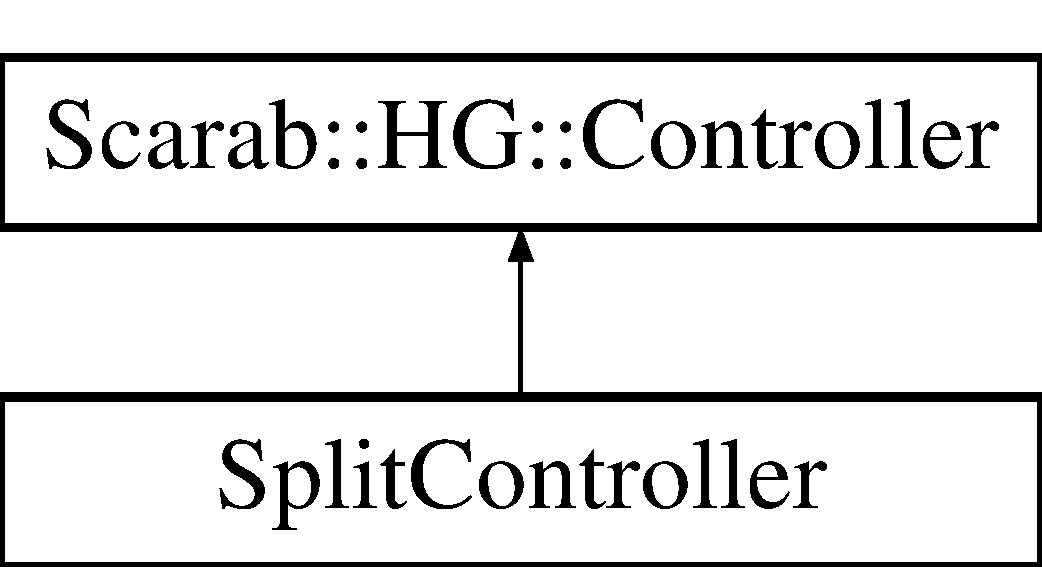
\includegraphics[height=2cm]{class_split_controller}
\end{center}
\end{figure}
\subsection*{Public Member Functions}
\begin{DoxyCompactItemize}
\item 
\hypertarget{class_split_controller_a511e733b586a24c2cad5ba16a6cb381b}{
{\bfseries SplitController} (const \hyperlink{class_subproblem}{Subproblem} \&s, const \hyperlink{class_forest_lattice}{ForestLattice} \&l, bool two\_\-classes)}
\label{class_split_controller_a511e733b586a24c2cad5ba16a6cb381b}

\item 
\hypertarget{class_split_controller_ac01bf4220c60c35f6862160dc7fcacc7}{
int {\bfseries project\_\-word} (int w) const }
\label{class_split_controller_ac01bf4220c60c35f6862160dc7fcacc7}

\item 
\hypertarget{class_split_controller_a272757bbbfaa9af9d2ee2262b03ef131}{
int {\bfseries size} () const }
\label{class_split_controller_a272757bbbfaa9af9d2ee2262b03ef131}

\item 
\hypertarget{class_split_controller_ad2aeeafdc31d48526be15a1b1a2e9931}{
int {\bfseries dim} () const }
\label{class_split_controller_ad2aeeafdc31d48526be15a1b1a2e9931}

\item 
\hypertarget{class_split_controller_a6ac91d8fd5fef735c6572c420a05bda4}{
void {\bfseries initialize\_\-hypotheses} (const \hyperlink{class_scarab_1_1_h_g_1_1_hypernode}{Hypernode} \&node, vector$<$ \hyperlink{struct_scarab_1_1_h_g_1_1_hypothesis}{Hypothesis} $\ast$ $>$ \&hyps, vector$<$ double $>$ \&scores) const }
\label{class_split_controller_a6ac91d8fd5fef735c6572c420a05bda4}

\item 
\hypertarget{class_split_controller_a58e535837326d733c98a193f2c7584c6}{
void {\bfseries initialize\_\-out\_\-root} (vector$<$ \hyperlink{struct_scarab_1_1_h_g_1_1_hypothesis}{Hypothesis} $\ast$ $>$ \&hyps, vector$<$ double $>$ \&scores) const }
\label{class_split_controller_a58e535837326d733c98a193f2c7584c6}

\item 
\hypertarget{class_split_controller_a2138b9bac43d19896f2bff71a619e9af}{
double {\bfseries find\_\-best} (vector$<$ \hyperlink{struct_scarab_1_1_h_g_1_1_hypothesis}{Hypothesis} $\ast$ $>$ \&root\_\-hyps, vector$<$ double $>$ \&scores, \hyperlink{struct_scarab_1_1_h_g_1_1_hypothesis}{Hypothesis} \&best\_\-hyp) const }
\label{class_split_controller_a2138b9bac43d19896f2bff71a619e9af}

\end{DoxyCompactItemize}


The documentation for this class was generated from the following file:\begin{DoxyCompactItemize}
\item 
trans\_\-decode/Decode.cpp\end{DoxyCompactItemize}

\hypertarget{class_split_heuristic}{
\section{SplitHeuristic Class Reference}
\label{class_split_heuristic}\index{SplitHeuristic@{SplitHeuristic}}
}
Inheritance diagram for SplitHeuristic:\begin{figure}[H]
\begin{center}
\leavevmode
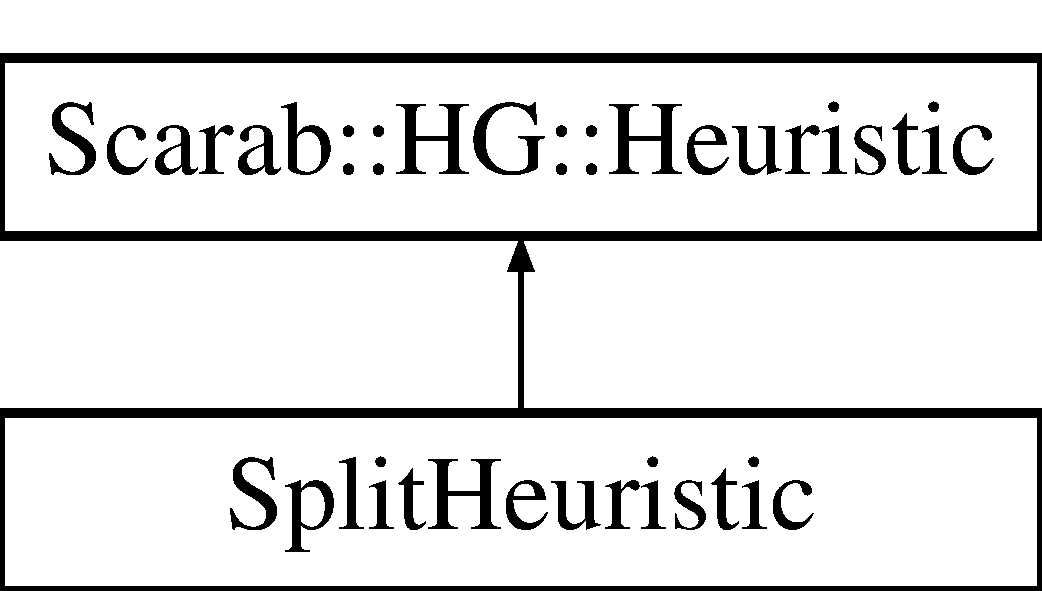
\includegraphics[height=2cm]{class_split_heuristic}
\end{center}
\end{figure}
\subsection*{Public Member Functions}
\begin{DoxyCompactItemize}
\item 
\hypertarget{class_split_heuristic_a8f58e4a4833f73460e2b2fb9c38448f1}{
{\bfseries SplitHeuristic} (const \hyperlink{class_cache}{Cache}$<$ \hyperlink{class_scarab_1_1_h_g_1_1_hypernode}{Hypernode}, \hyperlink{class_scarab_1_1_h_g_1_1_best_hyp}{BestHyp} $>$ \&outside\_\-scores, \hyperlink{class_cache}{Cache}$<$ \hyperlink{class_scarab_1_1_h_g_1_1_hyperedge}{Hyperedge}, vector$<$ \hyperlink{class_scarab_1_1_h_g_1_1_best_hyp}{BestHyp} $>$ $>$ \&outside\_\-edge\_\-scores)}
\label{class_split_heuristic_a8f58e4a4833f73460e2b2fb9c38448f1}

\item 
\hypertarget{class_split_heuristic_a0080cc4428de2635263f31d7931c3066}{
int {\bfseries lower\_\-id} (const \hyperlink{struct_scarab_1_1_h_g_1_1_hypothesis}{Hypothesis} \&hyp) const }
\label{class_split_heuristic_a0080cc4428de2635263f31d7931c3066}

\item 
\hypertarget{class_split_heuristic_a7117c99ce380835ed38aa02f82f8a04e}{
bool {\bfseries has\_\-value} (const \hyperlink{struct_scarab_1_1_h_g_1_1_location}{Location} \&l, const \hyperlink{struct_scarab_1_1_h_g_1_1_hypothesis}{Hypothesis} \&hyp) const }
\label{class_split_heuristic_a7117c99ce380835ed38aa02f82f8a04e}

\item 
\hypertarget{class_split_heuristic_ab64ec7cde28b49828bcde1ad97862cc2}{
double {\bfseries get\_\-value} (const \hyperlink{struct_scarab_1_1_h_g_1_1_location}{Location} \&l, const \hyperlink{struct_scarab_1_1_h_g_1_1_hypothesis}{Hypothesis} \&hyp) const }
\label{class_split_heuristic_ab64ec7cde28b49828bcde1ad97862cc2}

\end{DoxyCompactItemize}


The documentation for this class was generated from the following file:\begin{DoxyCompactItemize}
\item 
trans\_\-decode/Decode.cpp\end{DoxyCompactItemize}

\hypertarget{struct_scarab_1_1_h_g_1_1_state}{
\section{Scarab::HG::State Struct Reference}
\label{struct_scarab_1_1_h_g_1_1_state}\index{Scarab::HG::State@{Scarab::HG::State}}
}
\subsection*{Public Member Functions}
\begin{DoxyCompactItemize}
\item 
\hypertarget{struct_scarab_1_1_h_g_1_1_state_a61592030e999341da1e674274db11307}{
{\bfseries State} (const vector$<$ int $>$ \&ids, uint dim)}
\label{struct_scarab_1_1_h_g_1_1_state_a61592030e999341da1e674274db11307}

\item 
\hypertarget{struct_scarab_1_1_h_g_1_1_state_a6597ae0951c6d0c9146ae6bd5b91b52f}{
\hyperlink{struct_scarab_1_1_h_g_1_1_state}{State} {\bfseries project} (int split, int down\_\-to) const }
\label{struct_scarab_1_1_h_g_1_1_state_a6597ae0951c6d0c9146ae6bd5b91b52f}

\item 
\hypertarget{struct_scarab_1_1_h_g_1_1_state_ac7f5641edb1dd813dcac3b76be28d305}{
int {\bfseries id} () const }
\label{struct_scarab_1_1_h_g_1_1_state_ac7f5641edb1dd813dcac3b76be28d305}

\item 
\hypertarget{struct_scarab_1_1_h_g_1_1_state_a17d205eca9f3be9c01c7d41e3fe4d809}{
bool {\bfseries operator==} (const \hyperlink{struct_scarab_1_1_h_g_1_1_state}{State} \&other) const }
\label{struct_scarab_1_1_h_g_1_1_state_a17d205eca9f3be9c01c7d41e3fe4d809}

\item 
\hypertarget{struct_scarab_1_1_h_g_1_1_state_acd8ef3e5bd73ec5034de0d70f2bb2492}{
bool {\bfseries compatible} (const \hyperlink{struct_scarab_1_1_h_g_1_1_state}{State} \&other) const }
\label{struct_scarab_1_1_h_g_1_1_state_acd8ef3e5bd73ec5034de0d70f2bb2492}

\item 
\hypertarget{struct_scarab_1_1_h_g_1_1_state_abadb936b551a91d952af74b3bfc7d43d}{
bool {\bfseries operator$<$} (const \hyperlink{struct_scarab_1_1_h_g_1_1_state}{State} \&other) const }
\label{struct_scarab_1_1_h_g_1_1_state_abadb936b551a91d952af74b3bfc7d43d}

\item 
\hypertarget{struct_scarab_1_1_h_g_1_1_state_afc65eeacc345b5396a673e4328cccc11}{
int {\bfseries possible\_\-states} () const }
\label{struct_scarab_1_1_h_g_1_1_state_afc65eeacc345b5396a673e4328cccc11}

\end{DoxyCompactItemize}
\subsection*{Public Attributes}
\begin{DoxyCompactItemize}
\item 
\hypertarget{struct_scarab_1_1_h_g_1_1_state_a1c516b546a5e3de3a5f9bb8f39a3cf20}{
vector$<$ int $>$ {\bfseries \_\-state}}
\label{struct_scarab_1_1_h_g_1_1_state_a1c516b546a5e3de3a5f9bb8f39a3cf20}

\end{DoxyCompactItemize}
\subsection*{Protected Attributes}
\begin{DoxyCompactItemize}
\item 
\hypertarget{struct_scarab_1_1_h_g_1_1_state_ae3d755b161845bd295deae4096d4c9f8}{
uint {\bfseries \_\-dim}}
\label{struct_scarab_1_1_h_g_1_1_state_ae3d755b161845bd295deae4096d4c9f8}

\end{DoxyCompactItemize}
\subsection*{Friends}
\begin{DoxyCompactItemize}
\item 
\hypertarget{struct_scarab_1_1_h_g_1_1_state_a353ffb342165fcaec0e812d0288fc329}{
ostream \& {\bfseries operator$<$$<$} (ostream \&output, const \hyperlink{struct_scarab_1_1_h_g_1_1_state}{State} \&p)}
\label{struct_scarab_1_1_h_g_1_1_state_a353ffb342165fcaec0e812d0288fc329}

\end{DoxyCompactItemize}


The documentation for this struct was generated from the following file:\begin{DoxyCompactItemize}
\item 
hypergraph/Hypothesis.h\end{DoxyCompactItemize}

\hypertarget{struct_state}{
\section{State Struct Reference}
\label{struct_state}\index{State@{State}}
}
\subsection*{Public Member Functions}
\begin{DoxyCompactItemize}
\item 
\hypertarget{struct_state_aa536880320a9aff707fb1e6aab3f58d4}{
{\bfseries State} (int id\_\-, string label\_\-)}
\label{struct_state_aa536880320a9aff707fb1e6aab3f58d4}

\item 
\hypertarget{struct_state_aea25c6702974d1ac86358b4ba96d7891}{
int {\bfseries id} () const }
\label{struct_state_aea25c6702974d1ac86358b4ba96d7891}

\item 
\hypertarget{struct_state_a2809d0a34cd576cc5daaa7a6d0ffb2b5}{
string {\bfseries label} () const }
\label{struct_state_a2809d0a34cd576cc5daaa7a6d0ffb2b5}

\item 
\hypertarget{struct_state_a6687a56382a022034927ba43aad39524}{
bool {\bfseries operator==} (const \hyperlink{struct_state}{State} \&other) const }
\label{struct_state_a6687a56382a022034927ba43aad39524}

\end{DoxyCompactItemize}
\subsection*{Public Attributes}
\begin{DoxyCompactItemize}
\item 
\hypertarget{struct_state_ae0482e3d4b3db023647833efd344831a}{
int {\bfseries \_\-id}}
\label{struct_state_ae0482e3d4b3db023647833efd344831a}

\item 
\hypertarget{struct_state_a1bf6100c59d50bc94ba781230a85a2e5}{
string {\bfseries \_\-label}}
\label{struct_state_a1bf6100c59d50bc94ba781230a85a2e5}

\end{DoxyCompactItemize}


The documentation for this struct was generated from the following file:\begin{DoxyCompactItemize}
\item 
optimization/MRF.h\end{DoxyCompactItemize}

\hypertarget{class_store_cache}{
\section{StoreCache$<$ C, V $>$ Class Template Reference}
\label{class_store_cache}\index{StoreCache@{StoreCache}}
}
\subsection*{Public Member Functions}
\begin{DoxyCompactItemize}
\item 
\hypertarget{class_store_cache_adeb02113caf8141430705ec5bab08a54}{
{\bfseries StoreCache} (int size)}
\label{class_store_cache_adeb02113caf8141430705ec5bab08a54}

\item 
\hypertarget{class_store_cache_a5aaafba803337cf3547159a6ac70a0ab}{
void {\bfseries resize} (int size)}
\label{class_store_cache_a5aaafba803337cf3547159a6ac70a0ab}

\item 
\hypertarget{class_store_cache_aa4673d48544458b6b05770fe5970d961}{
int {\bfseries size} () const }
\label{class_store_cache_aa4673d48544458b6b05770fe5970d961}

\item 
\hypertarget{class_store_cache_a455dbf75e40300745b354fdcc039279a}{
V {\bfseries get\_\-value} (const C \&edge) const }
\label{class_store_cache_a455dbf75e40300745b354fdcc039279a}

\item 
\hypertarget{class_store_cache_a23309f685f0ba18912dcc2e8643de932}{
void {\bfseries set\_\-value} (const C \&edge, V val)}
\label{class_store_cache_a23309f685f0ba18912dcc2e8643de932}

\item 
\hypertarget{class_store_cache_aa1289fedb472667dfa926c1e00f22b95}{
bool {\bfseries has\_\-key} (const C \&edge) const }
\label{class_store_cache_aa1289fedb472667dfa926c1e00f22b95}

\item 
\hypertarget{class_store_cache_ad358ce23080bb52db50a55db583f1bba}{
bool {\bfseries has\_\-key} (int k) const }
\label{class_store_cache_ad358ce23080bb52db50a55db583f1bba}

\end{DoxyCompactItemize}
\subsection*{Public Attributes}
\begin{DoxyCompactItemize}
\item 
\hypertarget{class_store_cache_a99393733357e04fe79cf703d3f4d8f44}{
vector$<$ V $>$ {\bfseries store}}
\label{class_store_cache_a99393733357e04fe79cf703d3f4d8f44}

\item 
\hypertarget{class_store_cache_a0df08d5576ce34c4a8fd4f7428fd9ad3}{
vector$<$ C $>$ {\bfseries full\_\-keys}}
\label{class_store_cache_a0df08d5576ce34c4a8fd4f7428fd9ad3}

\item 
\hypertarget{class_store_cache_acdfad2c43fd63e37fbb818ce282f6493}{
vector$<$ bool $>$ {\bfseries has\_\-value}}
\label{class_store_cache_acdfad2c43fd63e37fbb818ce282f6493}

\end{DoxyCompactItemize}
\subsubsection*{template$<$class C, class V$>$ class StoreCache$<$ C, V $>$}



The documentation for this class was generated from the following file:\begin{DoxyCompactItemize}
\item 
hypergraph/EdgeCache.h\end{DoxyCompactItemize}

\hypertarget{class_subgradient}{
\section{Subgradient Class Reference}
\label{class_subgradient}\index{Subgradient@{Subgradient}}
}
\subsection*{Public Member Functions}
\begin{DoxyCompactItemize}
\item 
\hyperlink{class_subgradient_a2509e39964e1280532fd4994b3d747ce}{Subgradient} (\hyperlink{class_subgradient_producer}{SubgradientProducer} \&subgrad\_\-producer)
\item 
\hypertarget{class_subgradient_a183205851cdb362195baf914fb8d3ae0}{
void {\bfseries solve} (int example)}
\label{class_subgradient_a183205851cdb362195baf914fb8d3ae0}

\item 
bool \hyperlink{class_subgradient_a54907389766b702c467cf2ab20f8d051}{is\_\-stuck} () const 
\end{DoxyCompactItemize}


\subsection{Constructor \& Destructor Documentation}
\hypertarget{class_subgradient_a2509e39964e1280532fd4994b3d747ce}{
\index{Subgradient@{Subgradient}!Subgradient@{Subgradient}}
\index{Subgradient@{Subgradient}!Subgradient@{Subgradient}}
\subsubsection[{Subgradient}]{\setlength{\rightskip}{0pt plus 5cm}Subgradient::Subgradient ({\bf SubgradientProducer} \& {\em subgrad\_\-producer})\hspace{0.3cm}{\ttfamily  \mbox{[}inline\mbox{]}}}}
\label{class_subgradient_a2509e39964e1280532fd4994b3d747ce}

\begin{DoxyParams}{Parameters}
\item[{\em subgrad\_\-producer}]Gives the subgradient at the current position \end{DoxyParams}


\subsection{Member Function Documentation}
\hypertarget{class_subgradient_a54907389766b702c467cf2ab20f8d051}{
\index{Subgradient@{Subgradient}!is\_\-stuck@{is\_\-stuck}}
\index{is\_\-stuck@{is\_\-stuck}!Subgradient@{Subgradient}}
\subsubsection[{is\_\-stuck}]{\setlength{\rightskip}{0pt plus 5cm}bool Subgradient::is\_\-stuck () const\hspace{0.3cm}{\ttfamily  \mbox{[}inline\mbox{]}}}}
\label{class_subgradient_a54907389766b702c467cf2ab20f8d051}
As the optimization probably reached a fixed point

\begin{DoxyReturn}{Returns}
true when stuck 
\end{DoxyReturn}


The documentation for this class was generated from the following files:\begin{DoxyCompactItemize}
\item 
optimization/Subgradient.h\item 
optimization/Subgradient.cpp\end{DoxyCompactItemize}

\hypertarget{class_subgradient_producer}{
\section{SubgradientProducer Class Reference}
\label{class_subgradient_producer}\index{SubgradientProducer@{SubgradientProducer}}
}
Inheritance diagram for SubgradientProducer:\begin{figure}[H]
\begin{center}
\leavevmode
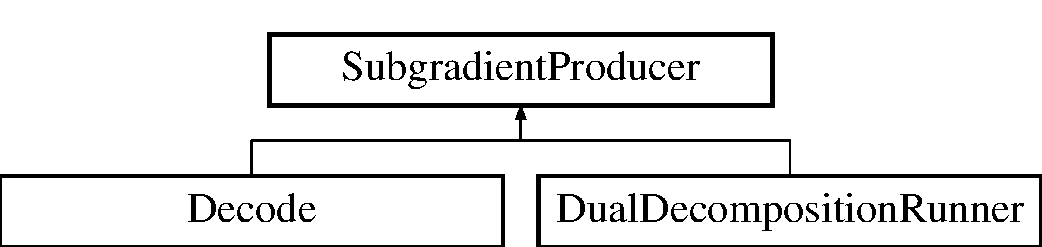
\includegraphics[height=2cm]{class_subgradient_producer}
\end{center}
\end{figure}
\subsection*{Public Member Functions}
\begin{DoxyCompactItemize}
\item 
\hypertarget{class_subgradient_producer_acea0e6ef35f9f3fd2f14872740471628}{
virtual void {\bfseries solve} (double \&primal, double \&dual, wvector \&, int, bool, bool \&)=0}
\label{class_subgradient_producer_acea0e6ef35f9f3fd2f14872740471628}

\item 
\hypertarget{class_subgradient_producer_a5b471526b337913722f56221b2461d89}{
virtual void {\bfseries update\_\-weights} (const wvector \&updates, wvector $\ast$weights)=0}
\label{class_subgradient_producer_a5b471526b337913722f56221b2461d89}

\end{DoxyCompactItemize}


The documentation for this class was generated from the following file:\begin{DoxyCompactItemize}
\item 
optimization/Subgradient.h\end{DoxyCompactItemize}

\hypertarget{class_subproblem}{
\section{Subproblem Class Reference}
\label{class_subproblem}\index{Subproblem@{Subproblem}}
}
\subsection*{Public Member Functions}
\begin{DoxyCompactItemize}
\item 
\hypertarget{class_subproblem_a1f76e6e7b079168299046c42e484c9cf}{
int {\bfseries overridden\_\-by} (int w) const }
\label{class_subproblem_a1f76e6e7b079168299046c42e484c9cf}

\item 
\hypertarget{class_subproblem_aba36ea76049a46e9ba1f0ac3ccec540a}{
void {\bfseries project} (int proj\_\-dim, vector$<$ int $>$ projection)}
\label{class_subproblem_aba36ea76049a46e9ba1f0ac3ccec540a}

\item 
\hypertarget{class_subproblem_a7c86b92cc388505602707376e52a0804}{
int {\bfseries project\_\-word} (int w) const }
\label{class_subproblem_a7c86b92cc388505602707376e52a0804}

\item 
\hypertarget{class_subproblem_a3f6d78f4567e70c35785d27a53a55490}{
void {\bfseries separate} (int w1, int w2)}
\label{class_subproblem_a3f6d78f4567e70c35785d27a53a55490}

\item 
\hypertarget{class_subproblem_a503126c48810484433fd6c3e428f6537}{
void {\bfseries projection\_\-with\_\-constraints} (int limit, int \&k, map$<$ int, set$<$ int $>$ $>$ \&constraints, vector$<$ int $>$ \&)}
\label{class_subproblem_a503126c48810484433fd6c3e428f6537}

\item 
\hypertarget{class_subproblem_a4c12e798de9d3e96d6935bd755f92a97}{
int {\bfseries best\_\-one} (int w1, int w2, int w3) const }
\label{class_subproblem_a4c12e798de9d3e96d6935bd755f92a97}

\item 
\hypertarget{class_subproblem_abf452bcac2a8a28adbdbffe402e64dde}{
int {\bfseries best\_\-two} (int w1, int w2, int w3) const }
\label{class_subproblem_abf452bcac2a8a28adbdbffe402e64dde}

\item 
\hypertarget{class_subproblem_a80e4996ec87d5c3501ef10abdd953260}{
double {\bfseries best\_\-score\_\-dim} (int w1, int d, int d2) const }
\label{class_subproblem_a80e4996ec87d5c3501ef10abdd953260}

\item 
\hypertarget{class_subproblem_a2e2a665cfdb9208f753eef143147d66c}{
double {\bfseries best\_\-score\_\-dim\_\-min} (int w1, vector$<$ int $>$ ds, vector$<$ int $>$ ds2) const }
\label{class_subproblem_a2e2a665cfdb9208f753eef143147d66c}

\item 
\hypertarget{class_subproblem_a2b43a2a68724d8eb624f6d81a7745b70}{
bool {\bfseries is\_\-new\_\-dim} (int w1, int d, int d2) const }
\label{class_subproblem_a2b43a2a68724d8eb624f6d81a7745b70}

\item 
\hypertarget{class_subproblem_a8359ae9db4d8a830d390312bc57eef6f}{
double {\bfseries best\_\-score} (int w1, int w2, int w3) const }
\label{class_subproblem_a8359ae9db4d8a830d390312bc57eef6f}

\item 
\hypertarget{class_subproblem_ae6b6a16e00079ebd5b56acbdfdaf3aab}{
{\bfseries Subproblem} (const \hyperlink{class_forest_lattice}{ForestLattice} $\ast$g, \hyperlink{class_ngram_cache}{NgramCache} $\ast$lm\_\-in, const \hyperlink{class_graph_decompose}{GraphDecompose} $\ast$gd\_\-in, const \hyperlink{class_cache}{Cache}$<$ \hyperlink{class_scarab_1_1_graph_1_1_graphnode}{Graphnode}, int $>$ \&word\_\-node\_\-cache\_\-in)}
\label{class_subproblem_ae6b6a16e00079ebd5b56acbdfdaf3aab}

\item 
\hypertarget{class_subproblem_adf6eb478907ed5c7c9f08a3cfcdfec76}{
void {\bfseries update\_\-weights} (vector$<$ int $>$ u\_\-pos, vector$<$ float $>$ u\_\-values, bool first)}
\label{class_subproblem_adf6eb478907ed5c7c9f08a3cfcdfec76}

\item 
\hypertarget{class_subproblem_a27c807a807f154ea28e7da7692466638}{
void {\bfseries solve} ()}
\label{class_subproblem_a27c807a807f154ea28e7da7692466638}

\item 
\hypertarget{class_subproblem_a8220595977ed219234d36dfadd0dde82}{
void {\bfseries initialize\_\-caches} ()}
\label{class_subproblem_a8220595977ed219234d36dfadd0dde82}

\item 
\hypertarget{class_subproblem_a9c57f3bd41e2788d9f393db8bbbe26ef}{
vector$<$ int $>$ {\bfseries get\_\-best\_\-nodes\_\-between} (int w1, int w2, bool first)}
\label{class_subproblem_a9c57f3bd41e2788d9f393db8bbbe26ef}

\item 
\hypertarget{class_subproblem_a3c426fd46fcacefc561b68f0fc111795}{
float {\bfseries get\_\-best\_\-bigram\_\-weight} (int w1, int w2, bool first)}
\label{class_subproblem_a3c426fd46fcacefc561b68f0fc111795}

\item 
\hypertarget{class_subproblem_adfba5511e1f004b989f7b2e03d998c4e}{
float {\bfseries primal\_\-score} (int word\mbox{[}$\,$\mbox{]}, int l)}
\label{class_subproblem_adfba5511e1f004b989f7b2e03d998c4e}

\item 
\hypertarget{class_subproblem_ab5e3b5e167561a79da1d815af120b6bd}{
double {\bfseries word\_\-prob} (int, int, int)}
\label{class_subproblem_ab5e3b5e167561a79da1d815af120b6bd}

\item 
\hypertarget{class_subproblem_acc456e9852f19058da2d884feec15679}{
double {\bfseries word\_\-backoff} (int)}
\label{class_subproblem_acc456e9852f19058da2d884feec15679}

\item 
\hypertarget{class_subproblem_afd0b98fea6ebb39ae5ad46d1010cb6a3}{
double {\bfseries word\_\-backoff\_\-two} (int i, int j)}
\label{class_subproblem_afd0b98fea6ebb39ae5ad46d1010cb6a3}

\item 
\hypertarget{class_subproblem_a32718cd109a52be59a7eecd3dc5f4c8a}{
double {\bfseries word\_\-prob\_\-reverse} (int, int, int)}
\label{class_subproblem_a32718cd109a52be59a7eecd3dc5f4c8a}

\item 
\hypertarget{class_subproblem_ab612e729dd11b5ac27ce9f67e0135c0a}{
double {\bfseries word\_\-prob\_\-bigram\_\-reverse} (int i, int j)}
\label{class_subproblem_ab612e729dd11b5ac27ce9f67e0135c0a}

\item 
\hypertarget{class_subproblem_a522f5f38fddff38424fe3958104a9612}{
int {\bfseries word\_\-bow\_\-reverse} (int i, int j, int k)}
\label{class_subproblem_a522f5f38fddff38424fe3958104a9612}

\item 
\hypertarget{class_subproblem_a1bce1ad18ee9c123677f39cccda7feb5}{
int {\bfseries word\_\-bow\_\-bigram\_\-reverse} (int i, int j)}
\label{class_subproblem_a1bce1ad18ee9c123677f39cccda7feb5}

\end{DoxyCompactItemize}
\subsection*{Public Attributes}
\begin{DoxyCompactItemize}
\item 
\hypertarget{class_subproblem_ab162552f8af9ee111227f6ec30b7a4f5}{
vector$<$ bool $>$ {\bfseries overridden}}
\label{class_subproblem_ab162552f8af9ee111227f6ec30b7a4f5}

\item 
\hypertarget{class_subproblem_aa981fb8aa661221937b3cd021d72c396}{
int {\bfseries projection\_\-dims}}
\label{class_subproblem_aa981fb8aa661221937b3cd021d72c396}

\end{DoxyCompactItemize}


The documentation for this class was generated from the following files:\begin{DoxyCompactItemize}
\item 
trans\_\-decode/dual\_\-subproblem.h\item 
trans\_\-decode/dual\_\-subproblem.cpp\end{DoxyCompactItemize}

\hypertarget{struct_tag}{
\section{Tag Struct Reference}
\label{struct_tag}\index{Tag@{Tag}}
}
\subsection*{Public Member Functions}
\begin{DoxyCompactItemize}
\item 
\hypertarget{struct_tag_ab32833339e272705062ac1a5d5f1ca10}{
{\bfseries Tag} (uint ind\_\-, POS tag\_\-, int len\_\-)}
\label{struct_tag_ab32833339e272705062ac1a5d5f1ca10}

\item 
\hypertarget{struct_tag_aed3aabe09176d4a6acbb2cc7b3170228}{
const bool {\bfseries operator$<$} (const \hyperlink{struct_tag}{Tag} \&other) const }
\label{struct_tag_aed3aabe09176d4a6acbb2cc7b3170228}

\item 
\hypertarget{struct_tag_a5458e1229013075f4597c1dba313ce83}{
int {\bfseries id} () const }
\label{struct_tag_a5458e1229013075f4597c1dba313ce83}

\end{DoxyCompactItemize}
\subsection*{Public Attributes}
\begin{DoxyCompactItemize}
\item 
\hypertarget{struct_tag_a072cbc6c6ac82c2398ad409a5eb28b71}{
int {\bfseries ind}}
\label{struct_tag_a072cbc6c6ac82c2398ad409a5eb28b71}

\item 
\hypertarget{struct_tag_a7b67562e1a664c9fed9afb74902b0fe5}{
int {\bfseries length}}
\label{struct_tag_a7b67562e1a664c9fed9afb74902b0fe5}

\item 
\hypertarget{struct_tag_a5f97e5e57a82b467da83f2990a276e81}{
POS {\bfseries tag}}
\label{struct_tag_a5f97e5e57a82b467da83f2990a276e81}

\end{DoxyCompactItemize}
\subsection*{Static Public Attributes}
\begin{DoxyCompactItemize}
\item 
\hypertarget{struct_tag_acb96fe3a41181e0e10628ae00fe63878}{
static const int {\bfseries MAX\_\-TAG} = 45}
\label{struct_tag_acb96fe3a41181e0e10628ae00fe63878}

\end{DoxyCompactItemize}


The documentation for this struct was generated from the following file:\begin{DoxyCompactItemize}
\item 
tagger/Tagger.h\end{DoxyCompactItemize}

\hypertarget{class_tag_constraints}{
\section{TagConstraints Class Reference}
\label{class_tag_constraints}\index{TagConstraints@{TagConstraints}}
}
\subsection*{Public Member Functions}
\begin{DoxyCompactItemize}
\item 
\hypertarget{class_tag_constraints_a58a2e5245400d411de24e36534d11945}{
{\bfseries TagConstraints} (int num\_\-tags)}
\label{class_tag_constraints_a58a2e5245400d411de24e36534d11945}

\item 
\hyperlink{class_cache}{EdgeCache} \hyperlink{class_tag_constraints_adec1a1de8fb49e79b52c4c93517414a0}{build\_\-tagger\_\-constraint\_\-vector} (int sent\_\-num, const \hyperlink{class_tagger}{Tagger} \&tagger, wvector \&orig\_\-weights) const 
\item 
\hypertarget{class_tag_constraints_acec3818d7505e9147828ab7cb3863001}{
wvector {\bfseries build\_\-tagger\_\-subgradient} (int sent\_\-num, const \hyperlink{class_tagger}{Tagger} \&tagger, const vector$<$ const \hyperlink{class_scarab_1_1_h_g_1_1_hyperedge}{Hyperedge} $\ast$ $>$ used\_\-edges) const }
\label{class_tag_constraints_acec3818d7505e9147828ab7cb3863001}

\item 
\hypertarget{class_tag_constraints_a8b8df130795f2fbc1ce2aac375dfc00a}{
void {\bfseries read\_\-from\_\-file} (string file\_\-name)}
\label{class_tag_constraints_a8b8df130795f2fbc1ce2aac375dfc00a}

\item 
\hypertarget{class_tag_constraints_a3e490a8d4d335ed4d04803fab0a82871}{
wvector {\bfseries solve\_\-hard} (wvector \&model) const }
\label{class_tag_constraints_a3e490a8d4d335ed4d04803fab0a82871}

\end{DoxyCompactItemize}
\subsection*{Public Attributes}
\begin{DoxyCompactItemize}
\item 
\hypertarget{class_tag_constraints_ad5aae083cb84eff2294ca7fbbd63cb67}{
vector$<$ \hyperlink{class_constraint_group}{ConstraintGroup} $>$ {\bfseries \_\-constraint\_\-struct}}
\label{class_tag_constraints_ad5aae083cb84eff2294ca7fbbd63cb67}

\item 
\hypertarget{class_tag_constraints_aba1f64a190bc4144fea14f01fe82ecc3}{
set$<$ int $>$ {\bfseries groups}}
\label{class_tag_constraints_aba1f64a190bc4144fea14f01fe82ecc3}

\item 
\hypertarget{class_tag_constraints_a83e2347bf237b00f02dc872c19fd4516}{
vector$<$ vector$<$ \hyperlink{struct_possible_tag}{PossibleTag} $>$ $>$ {\bfseries \_\-constrained\_\-words}}
\label{class_tag_constraints_a83e2347bf237b00f02dc872c19fd4516}

\item 
\hypertarget{class_tag_constraints_a29576d5022d4c5d03e6c8723669c3679}{
vector$<$ \hyperlink{struct_possible_tag}{PossibleTag} $>$ {\bfseries \_\-all\_\-constraints}}
\label{class_tag_constraints_a29576d5022d4c5d03e6c8723669c3679}

\item 
\hypertarget{class_tag_constraints_a8885071b73e699061347d17af6d9aa20}{
int {\bfseries \_\-num\_\-tags}}
\label{class_tag_constraints_a8885071b73e699061347d17af6d9aa20}

\end{DoxyCompactItemize}


\subsection{Member Function Documentation}
\hypertarget{class_tag_constraints_adec1a1de8fb49e79b52c4c93517414a0}{
\index{TagConstraints@{TagConstraints}!build\_\-tagger\_\-constraint\_\-vector@{build\_\-tagger\_\-constraint\_\-vector}}
\index{build\_\-tagger\_\-constraint\_\-vector@{build\_\-tagger\_\-constraint\_\-vector}!TagConstraints@{TagConstraints}}
\subsubsection[{build\_\-tagger\_\-constraint\_\-vector}]{\setlength{\rightskip}{0pt plus 5cm}{\bf EdgeCache} TagConstraints::build\_\-tagger\_\-constraint\_\-vector (int {\em sent\_\-num}, \/  const {\bf Tagger} \& {\em tagger}, \/  wvector \& {\em orig\_\-weights}) const}}
\label{class_tag_constraints_adec1a1de8fb49e79b52c4c93517414a0}
Given an sent\_\-num, the tagger, and a weight vector (indexed on constrained words) produce a weight vector indexed on edges. 

The documentation for this class was generated from the following files:\begin{DoxyCompactItemize}
\item 
tagger/TagConstraints.h\item 
tagger/TagConstraints.cpp\end{DoxyCompactItemize}

\hypertarget{class_tagger}{
\section{Tagger Class Reference}
\label{class_tagger}\index{Tagger@{Tagger}}
}
Inheritance diagram for Tagger:\begin{figure}[H]
\begin{center}
\leavevmode
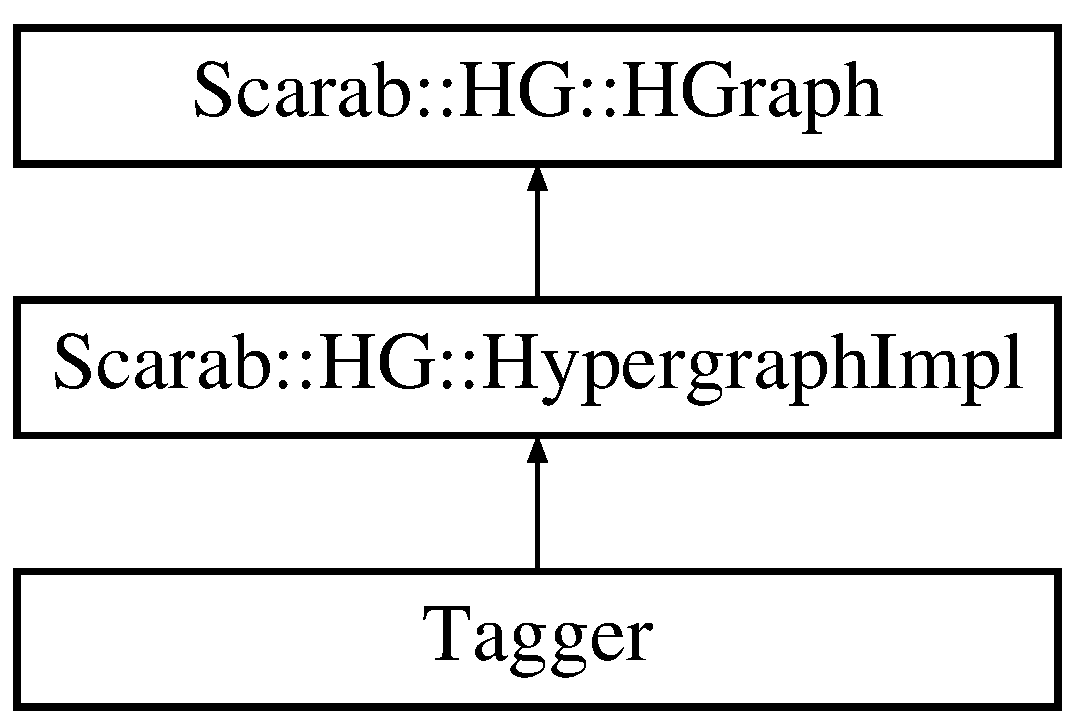
\includegraphics[height=3cm]{class_tagger}
\end{center}
\end{figure}
\subsection*{Public Member Functions}
\begin{DoxyCompactItemize}
\item 
\hypertarget{class_tagger_a6e812fd7e339a21155f7b30f04292be1}{
{\bfseries Tagger} (int num\_\-tags\_\-)}
\label{class_tagger_a6e812fd7e339a21155f7b30f04292be1}

\item 
void \hyperlink{class_tagger_a4ebe0aebd7c0392970b401a5a6c6cd72}{print} () const 
\item 
\hypertarget{class_tagger_afafa6e435d17467db344ca615f24746f}{
void {\bfseries set\_\-up} (const Hypergraph \&hgraph)}
\label{class_tagger_afafa6e435d17467db344ca615f24746f}

\item 
\hypertarget{class_tagger_ad694ed218149b86c4ef5253328a41c49}{
const Hypergraph \& {\bfseries hypergraph} () const }
\label{class_tagger_ad694ed218149b86c4ef5253328a41c49}

\item 
vector$<$ \hyperlink{struct_tag}{Tag} $>$ \hyperlink{class_tagger_ae1e3802fb545c3430ca4d52ea5fd95db}{tags} () const 
\item 
\hypertarget{class_tagger_a5da221998377bf36c84013ba0d471b36}{
uint {\bfseries num\_\-tags} () const }
\label{class_tagger_a5da221998377bf36c84013ba0d471b36}

\item 
\hypertarget{class_tagger_ae762dd21f446b9ec618b0b83204bdc2e}{
uint {\bfseries sent\_\-length} () const }
\label{class_tagger_ae762dd21f446b9ec618b0b83204bdc2e}

\item 
\hypertarget{class_tagger_af01daf511528271a118a281b8595e0df}{
\hyperlink{struct_tag}{Tag} {\bfseries make\_\-tag} (int ind, int tag) const }
\label{class_tagger_af01daf511528271a118a281b8595e0df}

\item 
\hypertarget{class_tagger_a26472c386e7f5eebcb05c9d1843c1975}{
const vector$<$ const \hyperlink{class_scarab_1_1_h_g_1_1_hyperedge}{Hyperedge} $\ast$ $>$ \& {\bfseries tag\_\-to\_\-edge} (const \hyperlink{struct_tag}{Tag} \&tag) const }
\label{class_tagger_a26472c386e7f5eebcb05c9d1843c1975}

\item 
\hypertarget{class_tagger_ae270a5be64b93945c180996aedcf6372}{
bool {\bfseries tag\_\-has\_\-edge} (const \hyperlink{struct_tag}{Tag} \&tag) const }
\label{class_tagger_ae270a5be64b93945c180996aedcf6372}

\item 
\hypertarget{class_tagger_ad615c8356f380baab01ae6675a25c409}{
const \hyperlink{struct_tag}{Tag} \& {\bfseries edge\_\-to\_\-tag} (const \hyperlink{class_scarab_1_1_h_g_1_1_hyperedge}{Hyperedge} \&edge) const }
\label{class_tagger_ad615c8356f380baab01ae6675a25c409}

\item 
\hypertarget{class_tagger_ad7f1dda6082e71cd113a3d77e9c33275}{
bool {\bfseries edge\_\-has\_\-tag} (const \hyperlink{class_scarab_1_1_h_g_1_1_hyperedge}{Hyperedge} \&edge) const }
\label{class_tagger_ad7f1dda6082e71cd113a3d77e9c33275}

\end{DoxyCompactItemize}
\subsection*{Public Attributes}
\begin{DoxyCompactItemize}
\item 
\hypertarget{class_tagger_a4bf3332c608c078cbb2d5692c4f13b43}{
int {\bfseries num\_\-tag}}
\label{class_tagger_a4bf3332c608c078cbb2d5692c4f13b43}

\end{DoxyCompactItemize}
\subsection*{Protected Member Functions}
\begin{DoxyCompactItemize}
\item 
\hypertarget{class_tagger_a305fd4cf75f2149a57109772e195eb47}{
void {\bfseries make\_\-edge} (const Hypergraph\_\-Edge \&edge, const \hyperlink{class_scarab_1_1_h_g_1_1_hyperedge}{Scarab::HG::Hyperedge} $\ast$our\_\-edge)}
\label{class_tagger_a305fd4cf75f2149a57109772e195eb47}

\end{DoxyCompactItemize}


\subsection{Member Function Documentation}
\hypertarget{class_tagger_a4ebe0aebd7c0392970b401a5a6c6cd72}{
\index{Tagger@{Tagger}!print@{print}}
\index{print@{print}!Tagger@{Tagger}}
\subsubsection[{print}]{\setlength{\rightskip}{0pt plus 5cm}void Tagger::print () const\hspace{0.3cm}{\ttfamily  \mbox{[}inline, virtual\mbox{]}}}}
\label{class_tagger_a4ebe0aebd7c0392970b401a5a6c6cd72}
Display the hypergraph for debugging. 

Implements \hyperlink{class_scarab_1_1_h_g_1_1_h_graph_ab5aa11c932b28864b56f28e0babbc1c1}{Scarab::HG::HGraph}.

\hypertarget{class_tagger_ae1e3802fb545c3430ca4d52ea5fd95db}{
\index{Tagger@{Tagger}!tags@{tags}}
\index{tags@{tags}!Tagger@{Tagger}}
\subsubsection[{tags}]{\setlength{\rightskip}{0pt plus 5cm}vector$<${\bf Tag} $>$ Tagger::tags () const\hspace{0.3cm}{\ttfamily  \mbox{[}inline\mbox{]}}}}
\label{class_tagger_ae1e3802fb545c3430ca4d52ea5fd95db}
Enumerate all the possible tags for this sentence

\begin{DoxyReturn}{Returns}
An enumerator to all the tags in the sentence 
\end{DoxyReturn}


The documentation for this class was generated from the following files:\begin{DoxyCompactItemize}
\item 
tagger/Tagger.h\item 
tagger/Tagger.cpp\end{DoxyCompactItemize}

\hypertarget{class_tagger_dual}{
\section{TaggerDual Class Reference}
\label{class_tagger_dual}\index{TaggerDual@{TaggerDual}}
}
Inheritance diagram for TaggerDual:\begin{figure}[H]
\begin{center}
\leavevmode
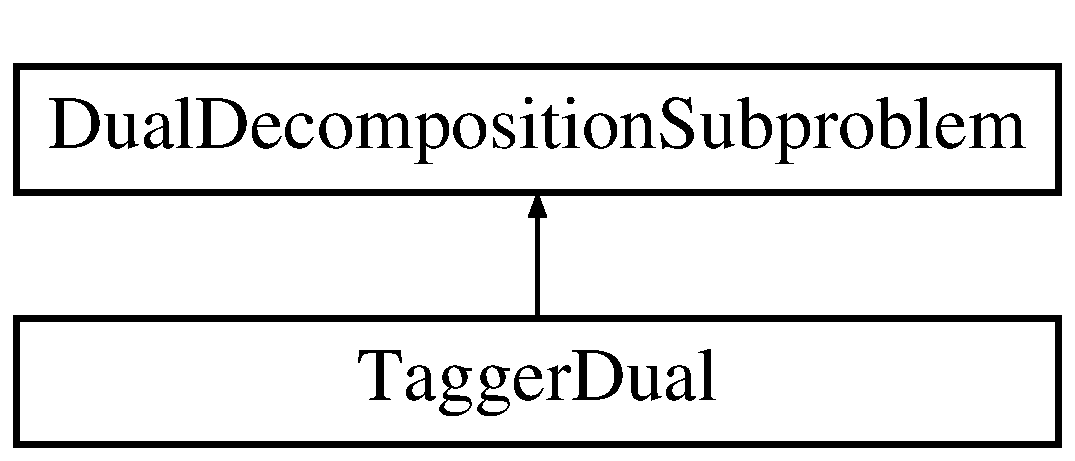
\includegraphics[height=2cm]{class_tagger_dual}
\end{center}
\end{figure}
\subsection*{Public Member Functions}
\begin{DoxyCompactItemize}
\item 
\hypertarget{class_tagger_dual_a2b16f45c3550e4f4871841c9ee02de4f}{
{\bfseries TaggerDual} (vector$<$ const \hyperlink{class_tagger}{Tagger} $\ast$ $>$ \&taggers, const wvector \&base\_\-weights, const \hyperlink{class_tag_constraints}{TagConstraints} \&cons)}
\label{class_tagger_dual_a2b16f45c3550e4f4871841c9ee02de4f}

\item 
\hypertarget{class_tagger_dual_a047785058d058492172280e50a8f4c1a}{
void {\bfseries solve} (double \&primal, double \&dual, wvector \&, int)}
\label{class_tagger_dual_a047785058d058492172280e50a8f4c1a}

\item 
\hypertarget{class_tagger_dual_a01f7705a69c7cc993268c6e66df57ae0}{
void {\bfseries update\_\-weights} (const wvector \&updates, wvector $\ast$weights, double mult)}
\label{class_tagger_dual_a01f7705a69c7cc993268c6e66df57ae0}

\end{DoxyCompactItemize}
\subsection*{Protected Attributes}
\begin{DoxyCompactItemize}
\item 
\hypertarget{class_tagger_dual_a0068b276abb09b34ab08e9cc14947ee3}{
const vector$<$ const \hyperlink{class_tagger}{Tagger} $\ast$ $>$ \& {\bfseries \_\-taggers}}
\label{class_tagger_dual_a0068b276abb09b34ab08e9cc14947ee3}

\item 
\hypertarget{class_tagger_dual_a0073fa0f694790d365ca959ed8386e26}{
const wvector \& {\bfseries \_\-base\_\-weights}}
\label{class_tagger_dual_a0073fa0f694790d365ca959ed8386e26}

\item 
\hypertarget{class_tagger_dual_ab8845276b234c329c967529091f51e8f}{
const \hyperlink{class_tag_constraints}{TagConstraints} \& {\bfseries \_\-tag\_\-constraints}}
\label{class_tagger_dual_ab8845276b234c329c967529091f51e8f}

\item 
\hypertarget{class_tagger_dual_a9974a79ebf2547f3e80e9d68d06b49be}{
wvector $\ast$ {\bfseries \_\-cur\_\-weights}}
\label{class_tagger_dual_a9974a79ebf2547f3e80e9d68d06b49be}

\item 
\hypertarget{class_tagger_dual_a57232f5a7702b7715f8517d408086dbe}{
vector$<$ wvector $>$ {\bfseries \_\-subgrad\_\-cache}}
\label{class_tagger_dual_a57232f5a7702b7715f8517d408086dbe}

\item 
\hypertarget{class_tagger_dual_a47cdc599b2c73836f33aa443053e3534}{
vector$<$ double $>$ {\bfseries \_\-primal\_\-cache}}
\label{class_tagger_dual_a47cdc599b2c73836f33aa443053e3534}

\item 
\hypertarget{class_tagger_dual_a4472c903ae391e7cc4912bc473a9eae2}{
vector$<$ double $>$ {\bfseries \_\-dual\_\-cache}}
\label{class_tagger_dual_a4472c903ae391e7cc4912bc473a9eae2}

\item 
\hypertarget{class_tagger_dual_a259d5ef5c5020c75a68527950ff41310}{
vector$<$ bool $>$ {\bfseries \_\-dirty\_\-cache}}
\label{class_tagger_dual_a259d5ef5c5020c75a68527950ff41310}

\end{DoxyCompactItemize}


The documentation for this class was generated from the following files:\begin{DoxyCompactItemize}
\item 
tagger/TagSolvers.h\item 
tagger/TagSolvers.cpp\end{DoxyCompactItemize}

\hypertarget{struct_tag_index}{
\section{TagIndex Struct Reference}
\label{struct_tag_index}\index{TagIndex@{TagIndex}}
}
\subsection*{Public Member Functions}
\begin{DoxyCompactItemize}
\item 
\hypertarget{struct_tag_index_a30a1bf326d593304ac3d950fd2b8be92}{
{\bfseries TagIndex} (int sent\_\-num\_\-, int ind\_\-, int tag\_\-)}
\label{struct_tag_index_a30a1bf326d593304ac3d950fd2b8be92}

\item 
\hypertarget{struct_tag_index_a7b858bbf2ed8ed6bb56d87db8d38aaf2}{
bool {\bfseries operator$<$} (const \hyperlink{struct_tag_index}{TagIndex} \&other) const }
\label{struct_tag_index_a7b858bbf2ed8ed6bb56d87db8d38aaf2}

\end{DoxyCompactItemize}
\subsection*{Public Attributes}
\begin{DoxyCompactItemize}
\item 
\hypertarget{struct_tag_index_a9bde045f6de7e99933920b883af894dc}{
int {\bfseries sent\_\-num}}
\label{struct_tag_index_a9bde045f6de7e99933920b883af894dc}

\item 
\hypertarget{struct_tag_index_ac9cd159e647314e5beaf7af6da56fa6e}{
int {\bfseries ind}}
\label{struct_tag_index_ac9cd159e647314e5beaf7af6da56fa6e}

\item 
\hypertarget{struct_tag_index_a1182f316658b96f36ecd7689d790f508}{
POS {\bfseries tag}}
\label{struct_tag_index_a1182f316658b96f36ecd7689d790f508}

\end{DoxyCompactItemize}


The documentation for this struct was generated from the following file:\begin{DoxyCompactItemize}
\item 
tagger/TagConstraints.h\end{DoxyCompactItemize}

\hypertarget{struct_scarab_1_1_h_g_1_1_tag_l_p}{
\section{Scarab::HG::TagLP Struct Reference}
\label{struct_scarab_1_1_h_g_1_1_tag_l_p}\index{Scarab::HG::TagLP@{Scarab::HG::TagLP}}
}
\subsection*{Public Member Functions}
\begin{DoxyCompactItemize}
\item 
\hypertarget{struct_scarab_1_1_h_g_1_1_tag_l_p_a529942132dc8900bd25d2acaef721694}{
{\bfseries TagLP} (const \hyperlink{class_tagger}{Tagger} \&parser, const \hyperlink{struct_scarab_1_1_h_g_1_1_hypergraph_l_p}{HypergraphLP} \&hyper\_\-lp)}
\label{struct_scarab_1_1_h_g_1_1_tag_l_p_a529942132dc8900bd25d2acaef721694}

\end{DoxyCompactItemize}
\subsection*{Public Attributes}
\begin{DoxyCompactItemize}
\item 
\hypertarget{struct_scarab_1_1_h_g_1_1_tag_l_p_a4e80b783a5dfce94abb94cb957a3fe50}{
\hyperlink{class_cache}{Cache}$<$ \hyperlink{struct_tag}{Tag}, GRBVar $>$ {\bfseries tag\_\-vars}}
\label{struct_scarab_1_1_h_g_1_1_tag_l_p_a4e80b783a5dfce94abb94cb957a3fe50}

\item 
\hypertarget{struct_scarab_1_1_h_g_1_1_tag_l_p_a137ec6055ea83b552c873dd19f203c15}{
const \hyperlink{class_tagger}{Tagger} \& {\bfseries p}}
\label{struct_scarab_1_1_h_g_1_1_tag_l_p_a137ec6055ea83b552c873dd19f203c15}

\item 
\hypertarget{struct_scarab_1_1_h_g_1_1_tag_l_p_a92b885535389aa44e450e8f4682bf543}{
const \hyperlink{struct_scarab_1_1_h_g_1_1_hypergraph_l_p}{HypergraphLP} \& {\bfseries h\_\-lp}}
\label{struct_scarab_1_1_h_g_1_1_tag_l_p_a92b885535389aa44e450e8f4682bf543}

\end{DoxyCompactItemize}


The documentation for this struct was generated from the following file:\begin{DoxyCompactItemize}
\item 
lp/TagLP.h\end{DoxyCompactItemize}

\hypertarget{class_scarab_1_1_h_g_1_1_tag_l_p_builder}{
\section{Scarab::HG::TagLPBuilder Class Reference}
\label{class_scarab_1_1_h_g_1_1_tag_l_p_builder}\index{Scarab::HG::TagLPBuilder@{Scarab::HG::TagLPBuilder}}
}
\subsection*{Static Public Member Functions}
\begin{DoxyCompactItemize}
\item 
\hypertarget{class_scarab_1_1_h_g_1_1_tag_l_p_builder_aa4990c224df5a1c82220a655ee51bd73}{
static void {\bfseries show\_\-results} (const \hyperlink{struct_scarab_1_1_h_g_1_1_tag_l_p}{TagLP} \&lp\_\-vars)}
\label{class_scarab_1_1_h_g_1_1_tag_l_p_builder_aa4990c224df5a1c82220a655ee51bd73}

\item 
\hypertarget{class_scarab_1_1_h_g_1_1_tag_l_p_builder_a9c0f3ee542cbbed34945b80932272cea}{
static \hyperlink{struct_scarab_1_1_h_g_1_1_tag_l_p}{TagLP} $\ast$ {\bfseries add\_\-tagging} (const \hyperlink{class_tagger}{Tagger} \&parser, const \hyperlink{class_cache}{Cache}$<$ \hyperlink{class_scarab_1_1_h_g_1_1_hyperedge}{Hyperedge}, double $>$ \&weights, string prefix, GRBModel \&model, int var\_\-type)}
\label{class_scarab_1_1_h_g_1_1_tag_l_p_builder_a9c0f3ee542cbbed34945b80932272cea}

\end{DoxyCompactItemize}


The documentation for this class was generated from the following files:\begin{DoxyCompactItemize}
\item 
lp/TagLP.h\item 
lp/TagLP.cpp\end{DoxyCompactItemize}

\hypertarget{class_tag_mrf_aligner}{
\section{TagMrfAligner Class Reference}
\label{class_tag_mrf_aligner}\index{TagMrfAligner@{TagMrfAligner}}
}
\subsection*{Public Member Functions}
\begin{DoxyCompactItemize}
\item 
\hypertarget{class_tag_mrf_aligner_ae2bae21b52efb547b46f2da80f61ec42}{
void {\bfseries build\_\-from\_\-constraints} (string file\_\-name)}
\label{class_tag_mrf_aligner_ae2bae21b52efb547b46f2da80f61ec42}

\item 
\hypertarget{class_tag_mrf_aligner_a5b6ecf59596d656333f8113f6f05eba4}{
bool {\bfseries align} (\hyperlink{struct_tag_index}{TagIndex} tag\_\-ind, \hyperlink{struct_mrf_index}{MrfIndex} \&mrf\_\-ind)}
\label{class_tag_mrf_aligner_a5b6ecf59596d656333f8113f6f05eba4}

\end{DoxyCompactItemize}
\subsection*{Public Attributes}
\begin{DoxyCompactItemize}
\item 
\hypertarget{class_tag_mrf_aligner_a8a5d34bcfecdfb8c3901297ad34e301d}{
vector$<$ \hyperlink{class_m_r_f}{MRF} $\ast$ $>$ {\bfseries mrf\_\-models}}
\label{class_tag_mrf_aligner_a8a5d34bcfecdfb8c3901297ad34e301d}

\item 
\hypertarget{class_tag_mrf_aligner_ae20f5a7d1131701986a36b70dca2c26f}{
vector$<$ vector$<$ \hyperlink{struct_tag_index}{TagIndex} $>$ $>$ {\bfseries tag\_\-constraints}}
\label{class_tag_mrf_aligner_ae20f5a7d1131701986a36b70dca2c26f}

\end{DoxyCompactItemize}


The documentation for this class was generated from the following files:\begin{DoxyCompactItemize}
\item 
tagger/TagConstraints.h\item 
tagger/TagConstraints.cpp\end{DoxyCompactItemize}

\hypertarget{class_tag_mrf_l_p}{
\section{TagMrfLP Class Reference}
\label{class_tag_mrf_l_p}\index{TagMrfLP@{TagMrfLP}}
}
\subsection*{Static Public Member Functions}
\begin{DoxyCompactItemize}
\item 
\hypertarget{class_tag_mrf_l_p_a7f9f963c533c5c712acca41db36f9a5a}{
static void {\bfseries align\_\-tag\_\-mrf} (const vector$<$ const \hyperlink{struct_m_r_f_l_p}{MRFLP} $\ast$ $>$ \&mrflp, const vector$<$ const \hyperlink{struct_scarab_1_1_h_g_1_1_tag_l_p}{TagLP} $\ast$ $>$ \&taglp, \hyperlink{class_tag_mrf_aligner}{TagMrfAligner} aligner, GRBModel \&model, int var\_\-type)}
\label{class_tag_mrf_l_p_a7f9f963c533c5c712acca41db36f9a5a}

\end{DoxyCompactItemize}


The documentation for this class was generated from the following file:\begin{DoxyCompactItemize}
\item 
lp/TagMrfLP.h\end{DoxyCompactItemize}

\printindex
\end{document}
